%%%%%%%%%%%%%%%%%%%%%%%%%5
%% abtex2-modelo-trabalho-academico.tex, v<VERSION> laurocesar
%% Copyright 2012-<COPYRIGHT_YEAR> by abnTeX2 group at http://www.abntex.net.br/
%%
%% This work may be distributed and/or modified under the
%% conditions of the LaTeX Project Public License, either version 1.3
%% of this license or (at your option) any later version.
%% The latest version of this license is in
%%   http://www.latex-project.org/lppl.txt
%% and version 1.3 or later is part of all distributions of LaTeX
%% version 2005/12/01 or later.
%%
%% This work has the LPPL maintenance status `maintained'.
%%
%% The Current Maintainer of this work is the abnTeX2 team, led
%% by Lauro César Araujo. Further information are available on
%% http://www.abntex.net.br/
%%
%% This work consists of the files abntex2-modelo-trabalho-academico.tex,
%% abntex2-modelo-include-comandos and abntex2-modelo-references.bib
%%

% ------------------------------------------------------------------------
% ------------------------------------------------------------------------
% abnTeX2: Modelo de Trabalho Academico (tese de doutorado, dissertacao de
% mestrado e trabalhos monograficos em geral) em conformidade com
% ABNT NBR 14724:2011: Informacao e documentacao - Trabalhos academicos -
% Apresentacao
% ------------------------------------------------------------------------
% ------------------------------------------------------------------------

\documentclass[
	% -- opções da classe memoir --
	12pt,				% tamanho da fonte
%  openright,			% capítulos começam em pág ímpar (insere página vazia caso preciso)
	oneside,			% para impressão em recto e verso use twoside
	a4paper,			% tamanho do papel.
	% -- opções da classe abntex2 --
	%chapter=TITLE,		% títulos de capítulos convertidos em letras maiúsculas
	%section=TITLE,		% títulos de seções convertidos em letras maiúsculas
	%subsection=TITLE,	% títulos de subseções convertidos em letras maiúsculas
	%subsubsection=TITLE,% títulos de subsubseções convertidos em letras maiúsculas
	% -- opções do pacote babel --
	english,			% idioma adicional para hifenização
	french,				% idioma adicional para hifenização
	spanish,			% idioma adicional para hifenização
	brazil				% o último idioma é o principal do documento
	]{abntex2}

% ---
% Pacotes básicos
% ---
\usepackage{times}			    % Usa fonte times
\renewcommand{\ABNTEXchapterfont}{\normalfont} % para aplicar a fonte escolhida em tudo
\usepackage[T1]{fontenc}		% Selecao de codigos de fonte.
\usepackage[utf8]{inputenc}		% Codificacao do documento (conversão automática dos acentos)
\usepackage{lastpage}			% Usado pela Ficha catalográfica
\usepackage{indentfirst}		% Indenta o primeiro parágrafo de cada seção.
\usepackage{color}				% Controle das cores
\usepackage{graphicx}			% Inclusão de gráficos
\usepackage{microtype} 			% para melhorias de justificação
% ---

% ---
% Pacotes adicionais, usados apenas no âmbito do Modelo Canônico do abnteX2
% ---
\usepackage{lipsum}				% para geração de dummy text
% ---

% ---
% Pacotes de citações
% ---
%\usepackage[brazilian,hyperpageref]{backref}	 % Paginas com as citações na bibl
%\usepackage[alf,abnt-nbr10520=1988]{abntex2cite}	% Citações padrão ABNT
\usepackage[alf]{abntex2cite}	% Citações padrão ABNT

% ---
% CONFIGURAÇÕES DE PACOTES
% ---

% ---
% Configurações do pacote backref
% Usado sem a opção hyperpageref de backref
\renewcommand{\backrefpagesname}{Citado na(s) página(s):~}
% Texto padrão antes do número das páginas
\renewcommand{\backref}{}
% Define os textos da citação
\renewcommand*{\backrefalt}[4]{
	\ifcase #1 %
		Nenhuma citação no texto.%
	\or
		Citado na página #2.%
	\else
		Citado #1 vezes nas páginas #2.%
	\fi}%
% ---

% ---
% Informações de dados para CAPA e FOLHA DE ROSTO
% ---
\titulo{Sentilytics: Análise Automatizada de Sentimentos em Redes Sociais}
\autor{José Alessandro Santos Santana}
\data{2025}
\local{Lagarto - SE}
\orientador{Prof.~Dr.~Gilson Pereira dos Santos Júnior}
\coorientador{}
\instituicao{%
  Instituto Federal de Sergipe
  \par
  Bacharelado em Sistemas de Informação
}
\tipotrabalho{Monografia}

% O preambulo deve conter o tipo do trabalho, o objetivo (propósito),
% o nome da instituição e a área de concentração.
% Esse texto irá compor a Folha de Rosto e Folha de Aprovação.
\preambulo{
Trabalho de Conclusão de Curso apresentado ao curso de Bacharelado em
Sistemas de Informação do Instituto Federal de Sergipe, Campus Lagarto,
como requisito parcial à obtenção do grau de bacharel em Sistemas de
Informação.
\newline\textbf{Área de concentração}: Computação.
}%% fim do preambulo




% ---
% Configurações de aparência do PDF final

% alterando o aspecto da cor azul
\definecolor{blue}{RGB}{41,5,195}

% informações do PDF
\makeatletter
\hypersetup{
     	%pagebackref=true,
		pdftitle={\@title},
		pdfauthor={\@author},
    	pdfsubject={\imprimirpreambulo},
	    pdfcreator={LaTeX with abnTeX2 and Limarka},
		pdfkeywords={abnt}{latex}{abntex}{abntex2}{trabalho acadêmico}{limarka},
		colorlinks=false,       		% false: boxed links; true: colored links
    	linkcolor=black,          	% color of internal links
    	citecolor=black,        		% color of links to bibliography
    	filecolor=black,      		% color of file links
		urlcolor=black,
		bookmarksdepth=4
}
\makeatother
% ---

% ---
% Possibilita criação de Quadros e Lista de quadros.
% Ver https://github.com/abntex/abntex2/issues/176
%
\newcommand{\quadroname}{Quadro}
\newcommand{\listofquadrosname}{Lista de quadros}

\newfloat[chapter]{quadro}{loq}{\quadroname}
\newlistof{listofquadros}{loq}{\listofquadrosname}
\newlistentry{quadro}{loq}{0}

% configurações para atender às regras da ABNT
\setfloatadjustment{quadro}{\centering}
\counterwithout{quadro}{chapter}
\renewcommand{\cftquadroname}{\quadroname\space}
\renewcommand*{\cftquadroaftersnum}{\hfill--\hfill}

% ---


% ---
% Espaçamentos entre linhas e parágrafos
% ---

% O tamanho do parágrafo é dado por:
\setlength{\parindent}{1.3cm}

% Controle do espaçamento entre um parágrafo e outro:
\setlength{\parskip}{0.2cm}  % tente também \onelineskip

% ---
% compila o indice
% ---
\makeindex
% ---

%---
% CONFIGURAÇÕES EXTRA DO LIMARKA
%---

% Configura citações de pandoc para 4cm à esquerda (utiliza o ambiente quote)
\renewenvironment{quote}
  {\small\list{}{\rightmargin=0.1cm \leftmargin=4cm}%
   \item\relax}
  {\endlist}

% Para incluir páginas PDF (ficha catalografica e folha de aprovação)
\usepackage[dvipsnames]{xcolor} % http://tex.stackexchange.com/questions/124636/package-xcolor-error-undefined-colors-maroon-royal-blue-when-master-has-pdf
\usepackage{pdfpages}
\usepackage{longtable,ltcaption,booktabs} % para as tabelas pandoc e quadros ABNT
%\usepackage{floatrow}
%\floatsetup[figure]{capposition=top}

% Para melhorar o visual do quadro
\usepackage{boldline}
\def\toprule{\hlineB{3}} % primeira linha mais gorda
\def\midrule{\hline}
\def\bottomrule{\hlineB{3}} % última linha mais gorda



% ---
% BUG: Imagens e tabelas apareciam no meio da página em branco
% https://github.com/abntex/trabalho-academico-limarka/issues/1
% O código a seguir posta imagens ou tabelas em página em branco no topo, em vez do meio (comportamento padrão)
\makeatletter
\setlength{\@fptop}{5pt} % Set distance from top of page to first float
\makeatother
% ---

% ---
% Usado pelo limarka como hook para criação de novas listas.
% https://github.com/abntex/trabalho-academico-limarka/issues/16
%
\newcommand{\listasdousuario}{}

% ---
% CUSTOMIZAÇÕES DO USUÁRIO (somente se existir arquivo config/latexcustomizacao.sty)
% ---
\IfFileExists{latexcustomizacao.sty}{\usepackage{latexcustomizacao}}{}

%%
%% Esse modelo é responsável pela impressão dos seguintes elementos:
%% Capa, Folha de rosto e Ficha catalográfica.

\special{dvipdfmx:config z 0}

% ----
% Início do documento
% ----
\begin{document}

% Seleciona o idioma do documento (conforme pacotes do babel)
%\selectlanguage{english}
\selectlanguage{brazil}

% Retira espaço extra obsoleto entre as frases.
\frenchspacing

% ----------------------------------------------------------
% ELEMENTOS PRÉ-TEXTUAIS
% ----------------------------------------------------------
% \pretextual

% ---
% Capa 
% ---
% Gerando capa abnTeX2
\imprimircapa

% ---

% ----------------------------------------------------------
% ELEMENTOS PRÉ-TEXTUAIS
% ----------------------------------------------------------
% \pretextual

% ---
% Folha de rosto: sempre será impressa
% ---

\imprimirfolhaderosto* % (o * indica que haverá a ficha catalográfica)

% ---
% Inserir a ficha catalográfica
% ---
% Provavelmente a biblioteca da sua universidade lhe fornecerá um PDF
% com a ficha catalográfica definitiva após a defesa do trabalho. Quando estiver
% com o documento, salve-o como PDF no diretório do seu projeto e substitua todo
% o conteúdo de implementação deste arquivo pelo comando abaixo:

\begin{fichacatalografica}
    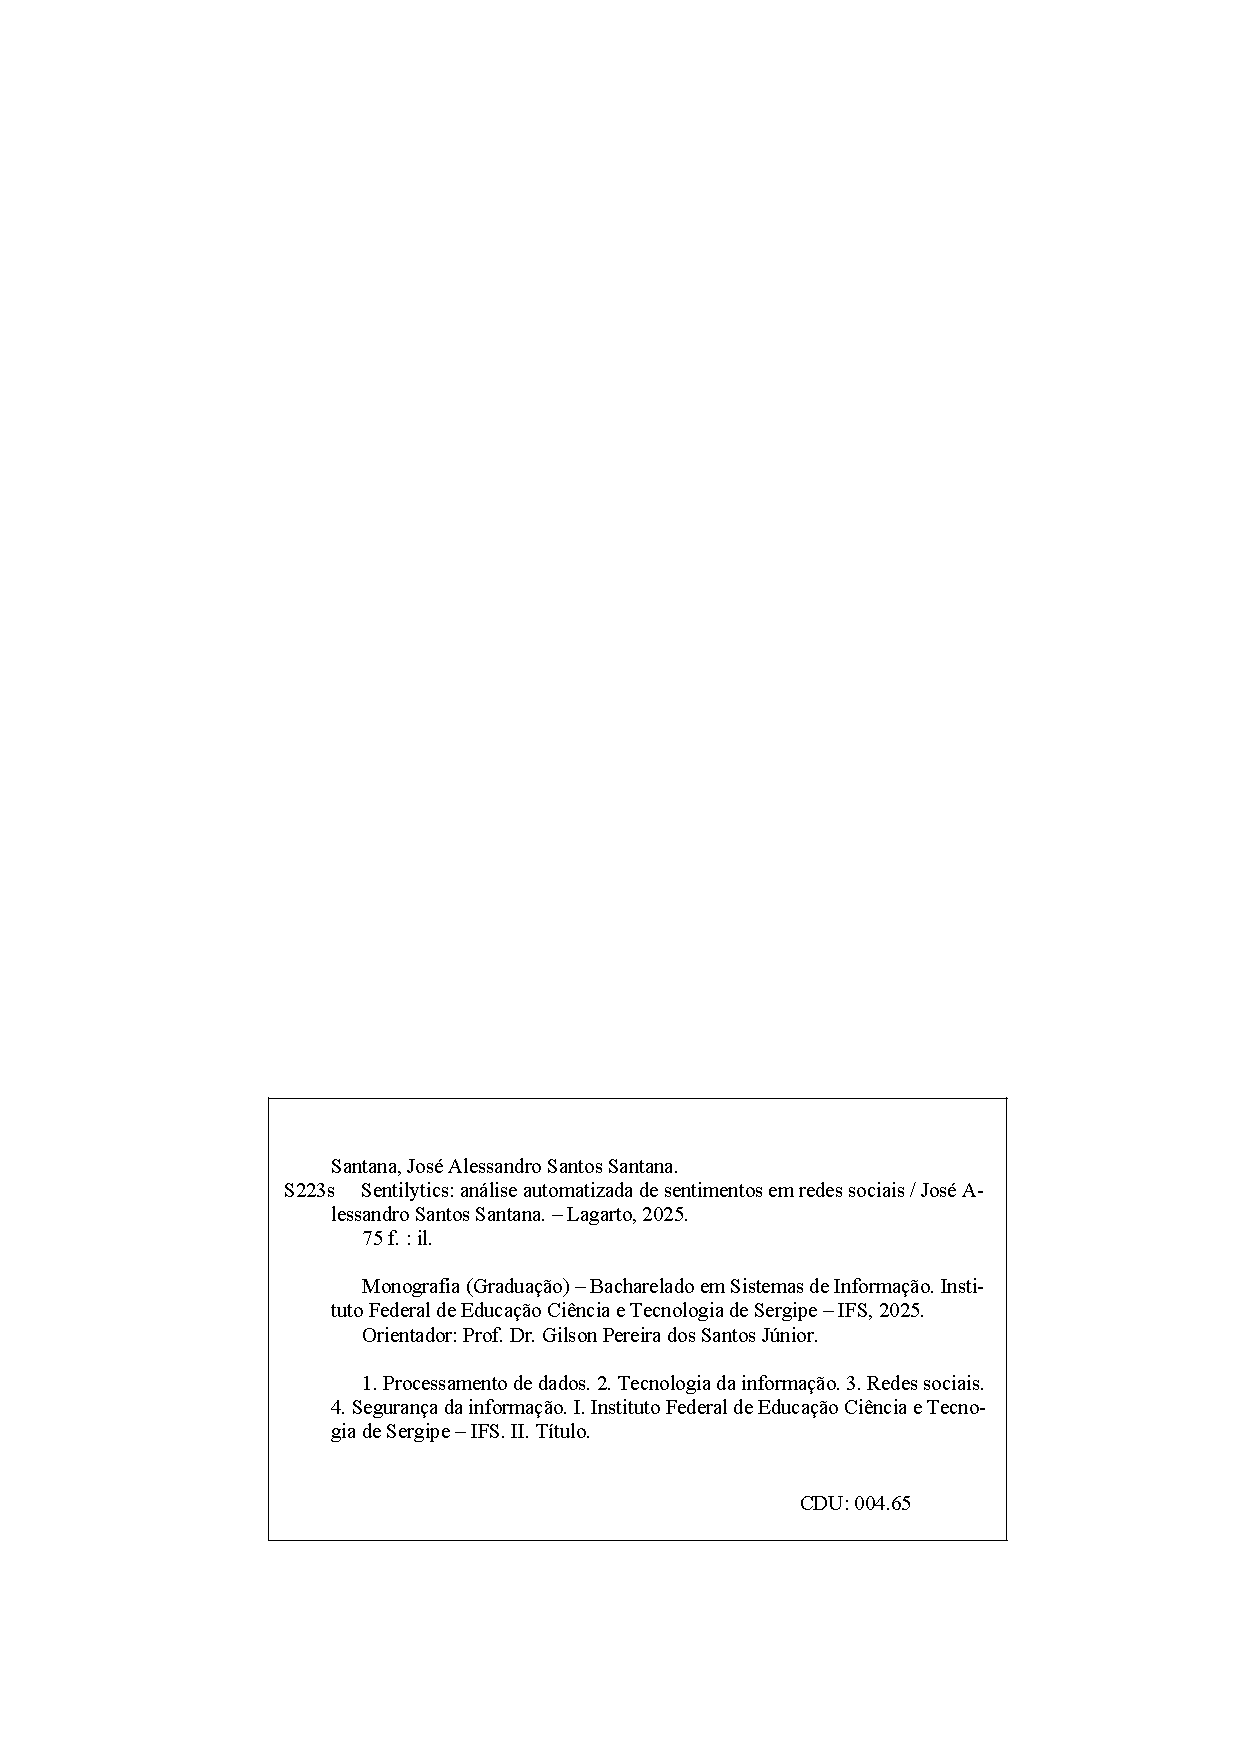
\includepdf{imagens/ficha-catalografica.pdf}
\end{fichacatalografica}

% ---


% ---
% ERRATA: Sem errata
% ---


% ---
% Folha de aprovação gerada
% ---

% Isto é um exemplo de Folha de aprovação, elemento obrigatório da NBR
% 14724/2011 (seção 4.2.1.3).
% Este modelo será utilizado antes da aprovação do trabalho.

\begin{folhadeaprovacao}

  \begin{center}
    {\ABNTEXchapterfont\large\imprimirautor}

    \vspace*{\fill}\vspace*{\fill}
    \begin{center}
      \ABNTEXchapterfont\bfseries\Large\imprimirtitulo
    \end{center}
    \vspace*{\fill}

    \hspace{.45\textwidth}
    \begin{minipage}{.5\textwidth}

    \imprimirpreambulo

    \end{minipage}%
    \vspace*{\fill}
   \end{center}

   Monografia aprovada. \imprimirlocal, 12/03/2025 de  de 2025:

   \assinatura{\textbf{\imprimirorientador} \\ Orientador}
   \assinatura{\textbf{Prof.~Me. George Leite Junior} \\ Convidado}
   \assinatura{\textbf{Prof.~Me. Gustavo da Silva Quirino} \\ Convidado}

   \begin{center}
    \vspace*{0.5cm}
    {\large\imprimirlocal}
    \par
    {\large\imprimirdata}
    \vspace*{1cm}
  \end{center}

\end{folhadeaprovacao}
% ---
% ---
% Dedicatória
% ---
% ---
% Agradecimentos
% ---
\begin{agradecimentos}

A jornada até a conclusão deste trabalho foi desafiadora, mas também
repleta de aprendizados, crescimento e apoio de pessoas especiais. Sem
elas, esse momento não teria o mesmo significado.

Primeiramente, agradeço à minha família, que sempre esteve ao meu lado,
me incentivando e me dando forças nos momentos mais difíceis. O apoio
incondicional e a paciência foram fundamentais para que eu pudesse
chegar até aqui.

Aos meus professores, que desempenharam um papel essencial na minha
formação acadêmica e profissional, transmitindo não apenas conhecimento,
mas também valores que levarei para toda a vida. Em especial, gostaria
de expressar minha gratidão ao professor George Leite Junior, que foi
muito mais do que um professor dentro da sala de aula. Seu exemplo e
ensinamentos ultrapassaram os limites da universidade, tornando-se um
verdadeiro mentor.

Não poderia deixar de agradecer também aos meus amigos Kamille Gomes
Bezerra e Ítalo Martins de Deus, que estiveram comigo durante toda essa
jornada na faculdade. Compartilhamos desafios, noites mal dormidas,
risadas e conquistas. Sem vocês, esse percurso teria sido muito mais
difícil.

Por fim, mas não menos importante, expresso meu profundo agradecimento
ao meu orientador, Gilson Pereira dos Santos Júnior, por toda a
paciência, dedicação e incentivo ao longo da elaboração deste trabalho.
Sua orientação foi essencial para que este projeto se tornasse
realidade.

A todos vocês, meu muito obrigado!

\end{agradecimentos}
% ---
% ---
% Epígrafe
% ---
% ---

% ---
% Resumo na língua vernácula (obrigatório)
% ---


% resumo em português
\setlength{\absparsep}{18pt} % ajusta o espaçamento dos parágrafos do resumo
\begin{resumo}

  As redes sociais tornaram-se ambientes fundamentais para a disseminação
  de opiniões e sentimentos, impactando áreas como política, economia e
  comportamento social. No entanto, a análise automatizada desses
  sentimentos ainda apresenta desafios, como a necessidade de ferramentas
  intuitivas e capazes de lidar com grandes volumes de dados. Diante desse
  cenário, este trabalho propõe o Sentilytics, uma aplicação desenvolvida
  para realizar a análise automatizada de sentimentos em redes sociais. A
  aplicação foi construída utilizando Spring Boot, Angular e Python,
  integrando a coleta de postagens, pré-processamento textual e
  classificação de sentimentos em um fluxo único e personalizável. Para
  avaliação da aplicação, foi realizado um estudo de caso sobre o debate
  do fim da escala 6x1, onde foram analisadas postagens coletadas do
  Bluesky. Os resultados demonstraram que o Sentilytics é uma solução
  eficiente para análise de sentimentos, proporcionando visualizações
  gráficas e \emph{insights} interpretáveis. Como limitações, a versão
  inicial da aplicação utiliza apenas o modelo VADER, que apresenta
  dificuldades na detecção de ironia e ambiguidade, e da coleta restrita
  ao Bluesky, reduzindo a diversidade de dados. Para trabalhos futuros,
  propõe-se a expansão para outras redes sociais e a inclusão de modelos
  mais robustos de análise de sentimentos.

 \textbf{Palavras-chave}: Análise de Sentimentos, Processamento de Linguagem Natural, Redes
Sociais, Bluesky
\end{resumo}


% ---
% Resumo em língua estrangeira (obrigatório)
% ---

% resumo em inglês
\begin{resumo}[Abstract]
 \begin{otherlanguage*}{english}
   Social media has become a fundamental environment for the dissemination
   of opinions and sentiments, impacting areas such as politics, economics,
   and social behavior. However, the automated analysis of these sentiments
   still presents challenges, such as the need for intuitive tools capable
   of handling large volumes of data. Given this scenario, this study
   proposes Sentilytics, an application developed to perform automated
   sentiment analysis on social media. The application was built using
   Spring Boot, Angular, and Python, integrating data collection, text
   preprocessing, and sentiment classification into a unified and
   customizable workflow. To evaluate the application, a case study was
   conducted on the debate surrounding the end of the 6x1 work schedule,
   analyzing posts collected from Bluesky. The results demonstrated that
   Sentilytics is an efficient solution for sentiment analysis, providing
   graphical visualizations and interpretable insights. Regarding
   limitations, the initial version of the application relies solely on the
   VADER model, which has difficulties detecting irony and ambiguity, and
   its data collection is restricted to Bluesky, limiting the diversity of
   datasets. For future work, it is proposed to expand the application to
   other social networks and include more advanced sentiment analysis
   models.

   \vspace{\onelineskip}
 
   \noindent 
   \textbf{Keywords}: Sentiment Analysis, Natural Language Processing, Social Networks,
Bluesky
 \end{otherlanguage*}
\end{resumo}


% ---

% ---
% Lista de ilustrações (opcional)
% ---
\pdfbookmark[0]{\listfigurename}{lof}
\listoffigures*
\cleardoublepage


% ---
% inserir lista de quadros
% ---
\pdfbookmark[0]{\listofquadrosname}{loq}
\listofquadros*
\cleardoublepage
% ---

% Carrega listas definidas pelo usuário em `latexcustomizacao.sty`
\listasdousuario
% ---
% Lista de tabelas (opcional): não utilizando
% ---

% ---
% Lista de abreviaturas e siglas (opcional)
% ---
\begin{siglas}
  \item[API] Application Programming Interface
  \item[BPMN] Business Process Model and Notation
  \item[CSV] Comma-Separated Values
  \item[BERT] Bidirectional Encoder Representations from Transformers
  \item[GPT] Generative Pre-trained Transformer
  \item[AMQP] Advanced Message Queuing Protocol
  \item[NLTK] Natural Language Toolkit
  \item[VS Code] Visual Studio Code
  \item[SSE] Server-Sent Events
  \item[SQL] Structured Query Language
  \item[JSON] JavaScript Object Notation
  \item[AI] Artificial Intelligence
  \item[VADER] Valence Aware Dictionary and sEntiment Reasoner
  \item[XML] Extensible Markup Language
\end{siglas}
% ---

% ---
% Lista de símbolos (opcional): AUSENTE
% ---
% ---
% Sumário
% ---
\pdfbookmark[0]{\contentsname}{toc}
\tableofcontents*
\cleardoublepage
% ---


% ----------------------------------------------------------
% ELEMENTOS TEXTUAIS
% ----------------------------------------------------------
\textual
\pagestyle{simple}                  % #17 Cabeçalho apenas com
\aliaspagestyle{chapter}{simple}    % a numeração das páginas


\hypertarget{introduuxe7uxe3o}{%
\chapter{Introdução}\label{introduuxe7uxe3o}}

As redes sociais é o ambiente, no meio digital, em que os indivíduos
expressam suas percepções e sentimentos sobre temas variados, desde
questões cotidianas até debates complexos de relevância nacional, como
mudanças trabalhistas ou propostas legislativas. É um espaço que
possibilita diferentes formas de socialização, no qual os participantes
são emissores e receptores no processo de comunicação. No Brasil, as
redes sociais desempenham um papel crucial como meio de comunicação e
tem se resignificado como um espaço ativo para compreensão da opinião
pública e articulação política. De acordo com
\citeonline{pompei2021redes}, as redes sociais digitais são um meio
dinâmico e multifacetado de interação, que possibilita o engajamento
social e a formação de identidades em um ambiente marcado pela
diversidade e pela troca constante de informações.

Além de seu papel na articulação política, as redes sociais também
exercem um impacto significativo na economia e no comportamento das
novas gerações. No campo econômico, esses espaços têm sido utilizados
por empresas para monitorar tendências de mercado, analisar a
receptividade de produtos e serviços, e engajar diretamente com
consumidores, moldando estratégias de marketing e consumo. Por outro
lado, para os jovens, as redes sociais representam não apenas um canal
de entretenimento, mas também um espaço de mobilização e conscientização
social. Esses espaços permitem que eles se envolvam ativamente em
discussões sobre temas globais, como mudanças climáticas, direitos
humanos e questões trabalhistas, como o debate em torno da escala 6x1,
ampliando o alcance e a visibilidade dessas pautas.

A análise desses sentimentos é essencial para compreender tendências,
identificar polarizações e auxiliar na tomada de decisões estratégicas
em áreas como comunicação, política e negócios.

Entretanto, a análise de sentimentos em redes sociais apresenta desafios
significativos. Muitas ferramentas existentes não oferecem uma solução
integrada e intuitiva para o processamento completo, desde a coleta de
dados até a classificação dos sentimentos. Frequentemente, esses
processos exigem que os usuários utilizem terminais e comandos técnicos
para aplicar funções básicas, o que pode dificultar o uso por parte de
profissionais ou pesquisadores com pouca familiaridade técnica. Além
disso, essas ferramentas muitas vezes não permitem personalização ou
integração direta com redes sociais.

Diante desse cenário, foi desenvolvido o Sentilytics, uma aplicação para
automatização da análise de sentimentos personalizadas em redes sociais.
O Sentilytics automatiza o processo desde a coleta de dados até a
análise final, com uma personalização completa que permite aos usuários
criar \emph{workflows}\footnote{Workflow pode ser definido como um
  conjunto de tarefas organizadas.} configuráveis com diferentes funções
de pré-processamento. Além disso, a ferramenta possui integração direta
com a rede social Bluesky, garantindo que o fluxo de trabalho seja
otimizado e acessível, mesmo para usuários com pouca experiência
técnica. Essa abordagem automatizada e personalizável busca atender às
demandas crescentes por análises eficientes e adaptadas à realidade
brasileira.

Para validar a aplicação, foi realizado um estudo de caso utilizando o
Sentilytics para analisar sentimentos relacionados ao fim da escala 6x1,
uma pauta atual e polarizadora no contexto trabalhista brasileiro. O
tema foi escolhido pela relevância, atualidade e quantitativo de
interações entre os usuários da rede, permitindo a identificação de
padrões de engajamento em um debate de grande impacto social.

\hypertarget{objetivo-geral}{%
\section{Objetivo Geral}\label{objetivo-geral}}

Analisar sentimentos de forma automatizada em redes sociais por meio de
uma solução integrada denominada Sentilytics.

\hypertarget{objetivos-especuxedficos}{%
\section{Objetivos Específicos}\label{objetivos-especuxedficos}}

Para alcançar o objetivo geral proposto, o presente trabalho foi
estruturado em etapas especificas necessárias para a construção e
validação da solução desenvolvida. A seguir, são apresentados os
objetivos específicos que direcionaram o desenvolvimento da solução e
realização do estudo de caso.

\begin{itemize}
\tightlist
\item
  Implementar a coleta automatizada de dados em redes sociais integradas
  à aplicação;
\item
  Desenvolver um módulo de pré-processamento customizável para
  normalização e remoção de stopwords;
\item
  Integrar o modelo de análise de sentimentos VADER à aplicação para
  classificar sentimentos;
\item
  Exibir os resultados da análise de sentimentos por meio de gráficos,
  tabelas e nuvens de palavras;
\item
  Avaliar a aplicação por meio de um estudo de caso sobre o debate do
  fim da escala 6x1.
\end{itemize}

\hypertarget{relevuxe2ncia-do-trabalho}{%
\section{Relevância do trabalho}\label{relevuxe2ncia-do-trabalho}}

A análise de sentimentos é um campo de pesquisa em constante
crescimento, especialmente no contexto das redes sociais, que são ricas
em dados emocionais e opinativos. Este trabalho contribui para a área
acadêmica ao propor uma solução integrada e automatizada, o Sentilytics,
que possibilita a coleta de dados diretamente do Bluesky, uma
alternativa viável em um cenário onde muitas plataformas tornaram o
acesso aos dados mais restrito ou pago. Além disso, a criação de
\emph{workflows} configuráveis oferecem uma abordagem prática para
superar as limitações técnicas frequentemente enfrentadas por
pesquisadores, simplificando etapas complexas e manuais.

O desenvolvimento do Sentilytics introduz uma abordagem modular da
arquitetura, construída com tecnologias como Spring Boot, RabbitMQ e
PostgreSQL, garante escalabilidade e flexibilidade para a incorporação
de novos modelos de análise de sentimentos ou tarefas de
pré-processamento, evidenciando o potencial de expansão da ferramenta
para diferentes contextos.

No contexto das redes sociais, que hoje são fundamentais para a formação
de opiniões e debates públicos, a análise de sentimentos desempenha um
papel central na compreensão de tendências e polarizações. Este trabalho
contribui diretamente para esse campo ao oferecer uma ferramenta que
possibilita a análise automatizada de dados emocionais expressos em
postagens. O Sentilytics pode ser utilizado para identificar sentimentos
predominantes, compreender padrões de engajamento e fornecer informações
úteis para tomadores de decisão, pesquisadores e organizações que
desejam entender a dinâmica social em torno de temas complexos.

A relevância deste trabalho vai além de seu impacto imediato,
demonstrando como soluções tecnológicas inovadoras podem ser aplicadas
para explorar questões sociais e emocionais em um ambiente digital cada
vez mais complexo. A flexibilidade e escalabilidade do Sentilytics abrem
espaço para sua aplicação em diferentes áreas, como marketing, economia,
política, psicologia social e ciência de dados, tornando-o uma
ferramenta promissora tanto para estudos acadêmicos quanto para
aplicações práticas.

\hypertarget{estrutura-do-trabalho}{%
\section{Estrutura do Trabalho}\label{estrutura-do-trabalho}}

Este trabalho está organizado em 5 capítulos, além desta introdução, que
apresenta o contexto do problema, os objetivos e a relevância do estudo.
No capítulo 2, é apresentada a fundamentação teórica, abordando temas
como a influência das redes sociais na sociedade, conceitos sobre
análise de sentimentos e sua realização em redes sociais. O capítulo 3
detalha a construção e a modelagem do Sentilytics, desde a definição dos
requisitos, diagramação até as interfaces gráficas. O capítulo 4 discute
a metodologia adotada no estudo de caso, incluindo a coleta de dados,
pré-processamento, análise de sentimentos, resultados obtidos. Por fim,
no capítulo 5, são apresentadas as conclusões do trabalho, bem como as
limitações encontradas e sugestões para trabalhos futuros.

\hypertarget{fundamentauxe7uxe3o-teuxf3rica}{%
\chapter{Fundamentação Teórica}\label{fundamentauxe7uxe3o-teuxf3rica}}

As redes sociais desempenham um papel central, pois são uma das
principais fontes de dados para a análise de sentimentos, um campo de
pesquisa em constante evolução. A crescente relevância das redes sociais
na sociedade, tanto como meio de comunicação quanto como espaço para
expressões emocionais e opinativas, reforça a necessidade de investigar
suas dinâmicas e impactos.

Além disso, a análise de sentimentos em redes sociais emerge como uma
ferramenta indispensável para interpretar as emoções expressas por seus
usuários, permitindo identificar tendências, polarizações e padrões
comportamentais. Este trabalho explora esses aspectos, contextualizando
a influência das redes sociais e apresentando os métodos e técnicas que
fundamentam a análise automatizada de sentimentos. Ao final, são
discutidos trabalhos relacionados que destacam as oportunidades e
desafios na aplicação de tecnologias voltadas para a interpretação
emocional no ambiente digital.

\hypertarget{a-influuxeancia-das-redes-sociais-na-sociedade}{%
\section{A influência das redes sociais na
sociedade}\label{a-influuxeancia-das-redes-sociais-na-sociedade}}

As redes sociais transformaram a forma como as pessoas se conectam,
interagem e compartilham informações. Definidas como plataformas
digitais que permitem a criação e a troca de conteúdo gerado por
usuários, essas redes têm um papel central na sociedade contemporânea.
Desde a sua popularização, passaram a influenciar comportamentos
individuais e coletivos, sendo utilizadas tanto para o entretenimento
quanto para atividades mais complexas, como comunicação empresarial,
articulação política e mobilização social. Redes sociais como Facebook,
Twitter, Instagram e, mais recentemente, Bluesky, desempenham um papel
essencial na disseminação de informações em tempo real, moldando
narrativas e fortalecendo o conceito de cidadania digital. Nesse
contexto, as redes sociais digitais não apenas facilitam a interação
entre indivíduos e grupos, mas também influenciam profundamente a
construção de identidades e a participação social, promovendo um
ambiente dinâmico de troca de informações e de expressões culturais
\cite{pompei2021redes}.

Um dos impactos mais significativos das redes sociais é a sua capacidade
de aproximar pessoas. Plataformas digitais permitem que indivíduos de
diferentes partes do mundo se conectem instantaneamente, formem
comunidades baseadas em interesses comuns e colaborem em projetos ou
causas coletivas. Para muitos, essas plataformas funcionam como um meio
de socialização, especialmente em contextos de distanciamento físico ou
isolamento social, como foi observado durante a pandemia da COVID-19.
Além disso, redes sociais têm potencial para dar voz a grupos
marginalizados, ampliando a inclusão e a representatividade em debates
públicos. Nesse sentido, as redes sociais digitais são ferramentas
poderosas na disseminação da informação e na construção de interações
entre indivíduos e instituições, favorecendo a comunicação instantânea e
criando redes de apoio e compartilhamento de experiências, o que
fortalece ainda mais a participação social \cite{lima2021redes}.

Por outro lado, as redes sociais também amplificam o fenômeno da
polarização, dificultando o diálogo e favorecendo a formação de ``bolhas
sociais''. Esse problema é agravado por modelos de negócios que
priorizam a atenção do usuário, reforçando conteúdos alinhados às suas
preferências e diminuindo o contato com perspectivas divergentes
\cite{de2020democracia}​. Assim, as redes podem, simultaneamente, unir
grupos com interesses semelhantes e afastar grupos com opiniões opostas,
contribuindo para o aumento de tensões sociais. Esse processo, conhecido
como formação de bolhas sociais, ocorre quando os algoritmos reforçam
interações entre pessoas com visões similares, reduzindo o contato com
perspectivas diferentes e criando ambientes digitais homogêneos que
intensificam a polarização.

Ademais, o mau uso das redes sociais representa um dos maiores desafios
da era digital. A proliferação de fake news, discursos de ódio,
cyberbullying e manipulação de informações são exemplos de como essas
plataformas podem ser usadas de forma nociva. Essas questões não apenas
afetam diretamente a saúde mental dos usuários, mas também geram um
ambiente digital que intensifica sentimentos de exclusão social e
polarização.

No contexto político, redes sociais têm sido utilizadas para disseminar
desinformação e manipular a opinião pública, especialmente em períodos
eleitorais, o que agrava a confiança nas instituições democráticas.
Esses problemas evidenciam a necessidade de desenvolver estratégias e
ferramentas que promovam o uso ético e responsável dessas plataformas,
bem como soluções que analisem e monitorem o conteúdo publicado,
identificando padrões nocivos e promovendo transparência
\cite{siqueira2024impacto}.

Dessa forma, as redes sociais exercem uma influência ambivalente na
sociedade: enquanto aproximam pessoas e promovem inclusão, também
apresentam desafios significativos, como a polarização e o uso
inadequado. Entender essas dinâmicas é essencial para o desenvolvimento
de tecnologias que possam auxiliar na interpretação do comportamento
humano e no monitoramento dos impactos sociais dessas plataformas. Na
seção 2.2, apresento os fundamentos da análise de sentimentos e sua
aplicação no contexto das redes sociais, destacando sua importância para
a interpretação de dados gerados nesses ambientes.

\hypertarget{anuxe1lise-de-sentimento-nas-redes-sociais}{%
\section{Análise de sentimento nas redes
sociais}\label{anuxe1lise-de-sentimento-nas-redes-sociais}}

Com o crescimento exponencial das redes sociais, estas plataformas se
tornaram uma fonte rica de dados sobre comportamentos, opiniões e
sentimentos da população. A análise de sentimentos emerge como uma
ferramenta essencial para interpretar essas interações, permitindo a
identificação de emoções expressas em textos publicados pelos usuários.
Esse processo ajuda a compreender tendências, polarizações e padrões
emocionais em diferentes contextos, como política, marketing e
comportamento social.

A análise de sentimentos é uma subárea da Processamento de Linguagem
Natural (PLN) que tem como objetivo interpretar e categorizar emoções ou
opiniões em textos. Essa abordagem permite identificar sentimentos e
classificar em positivos, negativos ou neutros. No contexto das redes
sociais, o PLN desempenha um papel crucial ao lidar com a variedade e
complexidade da linguagem utilizada. Essa integração entre análise de
sentimentos e PLN possibilita transformar dados não estruturados em
informações valiosas para entender dinâmicas sociais, tendências de
opinião e comportamentos em larga escala.

Entretanto, nas redes sociais, a análise de sentimentos enfrenta
desafios únicos devido à natureza não estruturada das postagens. De
acordo com \citeonline{santana2023capitulo}, o Processamento de
Linguagem Natural (PLN) em redes sociais é desafiador devido à
variabilidade na forma como as pessoas expressam ideias, utilizando
linguagem informal, gírias, emojis, abreviações e até mesmo sarcasmo.

Nesta seção, são explorados os conceitos fundamentais da análise de
sentimentos e do Processamento de Linguagem Natural (PLN), os métodos
utilizados para aplicação em redes sociais e os principais desafios
enfrentados, incluindo exemplos práticos e trabalhos relacionados que
fundamentam a relevância deste campo de estudo.

\hypertarget{anuxe1lise-de-sentimento}{%
\subsection{Análise de sentimento}\label{anuxe1lise-de-sentimento}}

A análise de sentimento, também conhecida como \emph{opinion mining}, é
uma subárea do Processamento de Linguagem Natural (PLN) que busca
identificar, extrair e classificar emoções ou opiniões expressas em
textos. Ela é amplamente utilizada para entender como as pessoas se
sentem em relação a produtos, serviços, marcas, eventos ou questões
sociais e políticas. No contexto digital, onde grandes volumes de texto
são produzidos diariamente, a análise de sentimento tem se tornado uma
ferramenta indispensável para organizações e pesquisadores interessados
em interpretar o comportamento e as percepções do público.

A base da análise de sentimento é classificar um texto em categorias
emocionais, como positivo, negativo ou neutro. O processo pode ser
realizado de forma manual, com especialistas analisando cada texto, ou
de forma automatizada, utilizando técnicas de processamento de linguagem
natural (PLN). Esse processo de análise pode ser realizado de diferentes
métodos, que variam em complexidade e precisão. Dentre essas abordagens,
a análise de sentimentos automatizada se destaca como foco deste
trabalho, pois permite processar grandes volumes de dados com maior
eficiência.

Para viabilizar a análise de sentimentos automatizada, o PLN emprega
diversas técnicas e algoritmos para pré-processar o texto de modo a
obter o melhor resultado possível. Atualmente podemos encontrar diversas
tarefas que podem ser utilizadas. \citeonline{lopes2024otimizaccao}
define 10 tarefas de pré-processamento para melhorar a qualidade dos
resultados obtidos na análise de sentimentos, são elas: tokenização, PoS
Tagging, Stop Words, Normalização de texto, Correção ortográfica,
Stemming, Lematização, Reconhecimento de Entidades Nomeadas (REN),
Desambiguação do sentido da palavra e Detecção de limite de sentença.

Cada etapa desempenha um papel fundamental na preparação do texto para a
análise de sentimentos. A tokenização, por exemplo, divide o texto em
unidades menores, como palavras ou frases, facilitando sua interpretação
pelos algoritmos. O PoS Tagging classifica cada palavra segundo sua
função gramatical, permitindo entender a estrutura da sentença. Já a
remoção de \emph{stop words} exclui palavras comuns que não carregam
significado relevante para o contexto da análise. Além disso, processos
como normalização de texto e correção ortográfica ajudam a uniformizar
os dados, reduzindo inconsistências que podem comprometer a precisão dos
modelos de PLN. Análise de sentimentos se beneficia diretamente dessas
etapas, pois a qualidade dos dados de entrada influencia a precisão dos
resultados obtidos.

Com os textos devidamente pré-processados, a análise de sentimentos pode
ser aplicada para identificar e classificar emoções expressas nas
publicações. Existem diferentes abordagens para essa tarefa, cada uma
com suas vantagens e limitações. Entre as principais, destacam-se os
métodos baseados em léxicos, que utilizam dicionários de palavras
associadas a sentimentos, e os métodos baseados em aprendizado de
máquina, que treinam modelos para interpretar padrões emocionais nos
textos.

A abordagem baseada em léxicos\footnote{Conjunto de palavras e
  expressões organizadas com abse em características específicas, como
  significado, categoria gramtical ou carga emocional.} utiliza
dicionários de palavras previamente categorizadas por suas conotações
emocionais (positivas, negativas ou neutras). Quando uma palavra do
texto corresponde a uma entrada no léxico, seu peso emocional é somado
ao cálculo do sentimento geral da frase ou do documento. Exemplos
incluem ferramentas como o VADER (Valence Aware Dictionary and sEntiment
Reasoner\footnote{Tradução livre: Dicionário Ciente de Valência e
  Raciocínio de Sentimentos.}), amplamente utilizada para análise de
textos curtos, como postagens em redes sociais.

Um léxico é desenvolvido com base em um corpus\footnote{Conjunto de
  textos utilizados para análise linguística ou treinamento de modelos
  de PLN. Pode ser composto por documentos, mensagens, publicações em
  redes sociais, entre outros formatos de texto.}, que consiste em um
grande conjunto de textos usados para treinar, testar ou validar o
próprio léxico. Geralmente, um corpus é anotado manualmente para indicar
sentimentos ou outras informações relevantes, servindo como fundamento
para a construção e validação do léxico. Esse processo garante que as
palavras e expressões incluídas no léxico possuam uma classificação de
sentimento precisa e contextualizada.

Outra possibilidade para realizar a análise de sentimento é a abordagem
baseada em aprendizado de máquina, que utiliza algoritmos treinados em
conjuntos de dados rotulados para identificar padrões no texto e
classificar os sentimentos de forma autônoma. Modelos como Naive Bayes,
Support Vector Machines (SVM) e, mais recentemente, redes neurais
profundas (BERT e GPT) têm sido amplamente aplicados para melhorar a
precisão da análise.

Além dessas, há abordagem híbridas, combinam métodos baseados em léxicos
e aprendizado de máquina para aproveitar as potencialidades de ambas as
técnicas. A hibridização de técnicas é especialmente útil em casos mais
complexos, como quando o texto contém ironias ou ambiguidades que não
podem ser captadas apenas por dicionários.

Cada abordagem mencionada apresenta vantagens e limitações, por exemplo,
métodos baseados em léxicos são rápidos e de fácil implementação, mas
tendem a ter dificuldades com ironia ou sarcasmo. Já os métodos baseados
em aprendizado de máquina oferecem maior precisão, porém, exigem
conjuntos de dados rotulados e maior poder computacional para
treinamento.

\hypertarget{anuxe1lise-de-sentimento-em-postagens-nas-redes-sociais}{%
\subsection{Análise de sentimento em postagens nas redes
sociais}\label{anuxe1lise-de-sentimento-em-postagens-nas-redes-sociais}}

As redes sociais são plataformas dinâmicas onde os usuários compartilham
opiniões, sentimentos e experiências de forma constante. Uma postagem em
redes sociais pode ser definida como um conteúdo textual, geralmente
curto, publicado por um usuário para expressar uma ideia ou opinião.
Essas postagens podem conter texto, elementos visuais (imagens, vídeos)
e simbólicos (emojis, hashtags), que enriquecem o significado da
mensagem. Exemplos incluem tweets no X (antigo Twitter), posts no
Reddit, publicações no Facebook e postagens no Bluesky.

\begin{figure}[htbp]
\hypertarget{processo_analise_sentimentos}{%
\caption{Processo realizado para análise de sentimentos}\label{processo_analise_sentimentos}
\begin{center}
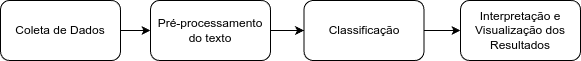
\includegraphics[scale=0.7]{imagens/processo_analise_sentimentos.png}
\end{center}
}
\legend{Fonte: Autor (2025).}
\end{figure}

Para viabilizar a análise de sentimentos nessas plataformas, diversos
estudos seguem um fluxo de processamento semelhante, conforme ilustrado
na \autoref{processo_analise_sentimentos}. O processo geralmente envolve
quatro etapas principais: coleta de dados, pré-processamento do texto,
classificação dos sentimentos e, por fim, interpretação e visualização
dos resultados. Na literatura, podemos identificar diferentes formas de
executar cada etapa, podendo ser executadas de forma manual ou
automatizada.

A etapa de coleta de dados inicia-se com a definição das plataformas de
onde as postagens serão extraídas. Atualmente, diversas redes sociais
são utilizadas para esse fim, sendo as mais comuns o X (antigo Twitter),
Facebook, Reddit, Instagram e Bluesky. O tipo de conteúdo postado nessas
plataformas varia conforme suas características, desde textos curtos e
objetivos, como no X e Reddit, até postagens mais extensas e multimídia,
como no Facebook e Instagram.

Além da variação no formato do conteúdo, a forma como os dados são
coletados também difere entre as plataformas. O X e o Reddit, por
exemplo, oferecem APIs pagas, o que inviabilizam pesquisas, como no caso
deste TCC. Em contrapartida, o Bluesky disponibiliza uma API gratuita,
permitindo a extração de dados sem custos. No entanto, sua baixa adesão
no Brasil pode ser um fator limitante, reduzindo a representatividade
dos dados coletados nessa rede.

Vale também notar que, para fins de pesquisa, alguns autores optam pelo
uso de web scraping como alternativa para a coleta de dados em redes
sociais. Essa abordagem permite extrair informações diretamente das
páginas da web, sem depender das APIs oficiais das plataformas. Contudo,
sua aplicação pode enfrentar desafios como limitações impostas por
termos de uso das redes sociais, bloqueios automatizados e necessidade
de ajustes constantes devido a mudanças na estrutura das páginas.

Na sequência, a etapa de pré-processamento é responsável por preparar os
textos antes de serem submetidos à classificação de sentimentos. As
tarefas executadas nessa fase podem variar conforme a fonte dos dados e
o classificador utilizado, adaptando-se às particularidades de cada
contexto. No caso das redes sociais, onde os textos costumam ser curtos,
informais, repletos de gírias, links e menções, algumas das técnicas
mais comuns incluem a remoção de stopwords, correção ortográfica e
tokenização (seja por palavras ou sentenças). Essas etapas são
fundamentais para reduzir ruídos e melhorar a precisão dos algoritmos de
análise de sentimentos.

Na etapa de classificação, é realizada a análise de sentimentos, onde os
textos pré-processados são avaliados e classificados de acordo com sua
polaridade emocional. Esse processo pode identificar se uma postagem
expressa um sentimento positivo, negativo ou neutro, utilizando
algoritmos baseados em léxicos, aprendizado de máquina ou abordagens
híbridas. A precisão da classificação depende da qualidade do
pré-processamento e do modelo utilizado, garantindo uma interpretação
mais confiável dos dados analisados.

Após a classificação, os resultados são interpretados e apresentados de
forma visual, por meio de gráficos, tabelas e nuvens de palavras. A
visualização adequada dos dados permite que pesquisadores e analistas
tomem decisões embasadas, identificando picos de polarização, temas
recorrentes e correlações entre sentimentos e eventos específicos.

Na literatura, essas etapas são implementadas de diversas formas, mas
geralmente seguem essa estrutura principal. Na seção de trabalhos
relacionados, serão discutidos diferentes sistemas que executam essas
etapas de maneira totalmente automatizada ou parcialmente manual, cada
um apresentando vantagens e limitações específicas. A comparação entre
essas abordagens permite compreender os desafios e avanços na área,
destacando como diferentes estratégias impactam a eficácia da análise de
sentimentos.

\hypertarget{trabalhos-relacionados-sobre-anuxe1lise-de-sentimentos-em-redes-sociais}{%
\subsection{Trabalhos relacionados sobre análise de sentimentos em redes
sociais}\label{trabalhos-relacionados-sobre-anuxe1lise-de-sentimentos-em-redes-sociais}}

A análise de sentimentos em redes sociais é um campo de pesquisa
amplamente explorado na literatura devido à crescente importância dessas
plataformas como fontes de dados emocionais e opinativos. Diversos
trabalhos já foram realizados para desenvolver e aprimorar métodos de
análise automatizada de sentimentos, bem como para entender o
comportamento dos usuários em ambientes digitais. Esta seção apresenta
uma revisão de estudos relacionados, destacando contribuições relevantes
na área, com foco em duas abordagens principais: a análise automática de
sentimentos, os estudos aplicados às redes sociais, que exploram as
especificidades desses ambientes e os desafios únicos associados à
análise de seus dados.

É importante ressaltar que os trabalhos relacionados que dependem da API
do X (antigo Twitter) para coletar dados e realizar análises podem
enfrentar restrições significativas, especialmente após a recente
implementação de um modelo pago para acesso. Essa limitação torna
algumas soluções menos acessíveis, sobretudo para pesquisadores e
pequenas organizações que não possuem recursos para adquirir planos
pagos. Como consequência, o uso de alternativas que não dependam
exclusivamente dessa API torna-se uma consideração relevante para
garantir maior flexibilidade na análise de dados em redes sociais.

No trabalho de \citeonline{malheiros2013ferramenta}, é apresentada uma
ferramenta de análise de sentimentos em mensagens de redes sociais
utilizando o SenticNet como base de conhecimento. A abordagem proposta
permite a classificação de sentimentos a partir da polaridade associada
a palavras e expressões presentes na base de dados, oferecendo um
processamento eficiente para grandes volumes de mensagens. Ainda assim,
a ferramenta apresenta algumas limitações, como a dependência exclusiva
do SenticNet, que restringe sua capacidade de análise a termos
previamente registrados na base, dificultando a adaptação a novos
contextos ou variações linguísticas. Além de que, sua aplicação inicial
foi voltada apenas para mensagens em inglês, o que limita sua
aplicabilidade em cenários multilíngues.

No ano seguinte \citeonline{malheiros2014emotte}, apresentada a
ferramenta web Emotte, desenvolvida para análise de sentimentos em
tweets da plataforma X. Utilizando técnicas de aprendizado de máquina e
processamento de linguagem natural, a ferramenta realiza a classificação
de sentimentos em tempo real. Contudo, o Emotte apresenta limitações,
como a aplicação de um conjunto fixo de tarefas de pré-processamento,
sem oferecer aos usuários a flexibilidade de personalizá-las de forma
simplificada.

\citeonline{vaillant2022ferramenta} também aborda a análise de
sentimentos no X, nesta caso, utilizando um modelo de aprendizado de
máquina supervisionado para a classificação de sentimentos. Todavia, sua
aplicação depende de um conjunto de dados previamente rotulado para
treinamento, o que pode limitar sua flexibilidade. Além do mais, não há
suporte para personalização do fluxo de pré-processamento.

No trabalho de \citeonline{moreira2024analise}, é apresentada uma
abordagem para a análise de sentimentos utilizando a ferramenta Orange
Datamining, essa ferramenta permite por meio de addons realizar a
análise de sentimentos, explorando diferentes métodos baseados em
léxico, como VADER, Liu \& Hu, SentiArt e Multilingual Sentiment. O
estudo avalia a eficácia da ferramenta ao analisar respostas discursivas
de alunos sobre uma disciplina de programação, incluindo a comparação
entre resultados obtidos em português e suas traduções para o inglês.
Embora a ferramenta ofereça suporte a múltiplos métodos, sua aplicação
apresenta algumas limitações, como a necessidade de tradução dos textos
para o inglês em algumas abordagens, o que pode introduzir distorções na
classificação emocional. Além de tudo, a ferramenta não possui uma
integração direta para coleta automatizada de dados, restringindo sua
aplicabilidade para estudos que exigem análise em grandes volumes de
texto.

O trabalho de \citeonline{dosferramenta} propõe uma ferramenta para
análise de sentimentos de tweets em português, com foco na coleta e
classificação automática das postagens em categorias de sentimentos
positivo e negativo. A abordagem adotada utiliza um classificador
baseado no Naïve Bayes, treinado com um conjunto de dados previamente
rotulado, além de realizar a coleta das postagens por meio da API do X.

O trabalho de \citeonline{gamallo2017linguakit} apresenta o LinguaKit,
uma suíte de ferramentas multilingues para análise linguística e
extração de informações, que inclui módulos para lematização,
etiquetagem morfossintática, análise sintática e correção gramatical.
Além disto, a ferramenta conta com um módulo dedicado à análise de
sentimentos, utilizando um classificador bayesiano combinado com léxicos
de polaridade e regras sintáticas para intensificação ou modificação de
sentimentos. Porém, embora ofereça um conjunto abrangente de
funcionalidades, a abordagem utilizada depende de modelos baseados em
regras e aprendizado supervisionado, o que pode limitar sua
flexibilidade para adaptação a novos domínios sem a necessidade de
reconfiguração manual. Ademais, a suíte exige uma configuração detalhada
e não dispõe de integração direta com redes sociais para coleta
automatizada de dados, o que pode dificultar sua aplicação em análises
contínuas e em larga escala.

O trabalho de \citeonline{deaplicando} propõe uma abordagem diferenciada
para a análise de sentimentos no X, utilizando a API da plataforma para
coletar os dados, aplicar o pré-processamento e exibir os resultados.
Para isso, a implementação foi realizada no Google Colab, uma ferramenta
que permite a execução de código Python de forma estruturada e
interativa. A análise dos sentimentos foi conduzida dentro do ambiente
do Colab, por meio da geração de nuvens de palavras e da exibição de
gráficos gerais.

\begin{figure}[htbp]
\hypertarget{google_colab}{%
\caption{Goggle Colab com algoritmo python para criação de um dataframe}\label{google_colab}
\begin{center}
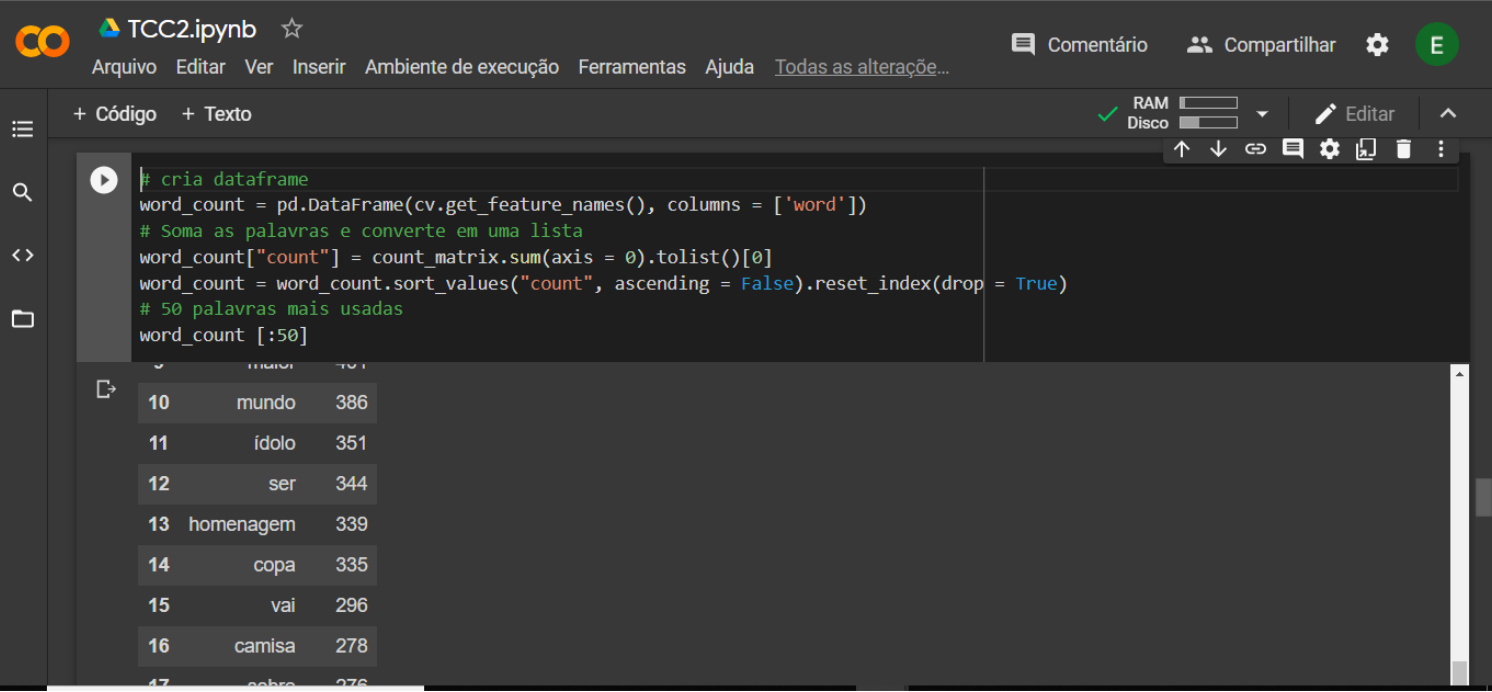
\includegraphics[scale=0.3]{imagens/google_colab.png}
\end{center}
}
\legend{Fonte: \cite{deaplicando}.}
\end{figure}

Para utilizar essa abordagem, o usuário precisa acessar o Google Colab,
carregar o código Python disponibilizado pelo autor e configurar os
parâmetros necessários para a coleta e análise dos dados. Inicialmente,
é necessário estabelecer a conexão com a API do X, fornecendo as
credenciais de acesso e definindo os critérios de busca para a extração
dos \emph{tweets}. Em seguida, o usuário deve executar manualmente cada
célula do \emph{notebook}, garantindo que os dados sejam coletados,
pré-processados e, posteriormente, analisados por meio de gráficos e
nuvens de palavras geradas pelo \emph{script}. Esse processo, apesar de
estruturado, exige um nível intermediário de familiaridade com Python e
com o ambiente do Google Colab, o que pode representar uma barreira para
pesquisadores sem experiência prévia em programação.

O trabalho de \citeonline{bilo2023ferramenta} apresenta uma ferramenta
desenvolvida para análise de sentimentos em postagens realizadas no
ambiente virtual de aprendizagem Moodle. O objetivo principal da solução
é auxiliar professores na compreensão das emoções dos alunos, permitindo
a adaptação das metodologias de ensino com base nas interações
realizadas nos fóruns, mensagens privadas e chats da plataforma. Para
isso, a ferramenta utiliza técnicas de processamento de linguagem
natural e diferentes APIs para classificar os sentimentos expressos
pelos alunos. A interface desenvolvida possibilita a visualização dos
resultados em gráficos interativos, permitindo um monitoramento
detalhado do estado emocional da turma.

Embora a abordagem apresentada seja eficaz para o contexto educacional,
a ferramenta apresenta algumas limitações. Primeiramente, sua
aplicabilidade está restrita ao ambiente do Moodle, limitando sua
utilização em outras plataformas de redes sociais ou sistemas de
discussão. Além de que, a análise de sentimentos depende de múltiplas
APIs externas, o que pode impactar a flexibilidade da ferramenta e sua
adaptabilidade a novos cenários. Outra limitação relevante é que o
sistema exige a instalação local nos dispositivos dos professores, o que
pode representar uma barreira para usuários com menos experiência
técnica.

O trabalho de \citeonline{da2010bestchoice} apresenta o BestChoice, um
sistema desenvolvido para análise de sentimentos em textos extraídos da
web, com foco na classificação automática de opiniões sobre produtos e
serviços. A abordagem proposta utiliza técnicas de Processamento de
Linguagem Natural (PLN) e o SentiWordNet para atribuir polaridade aos
textos, permitindo que as avaliações sejam classificadas sem a
necessidade de intervenção manual. Essa solução visa otimizar o processo
de análise de sentimentos. Todavia, apesar de sua eficiência para o
contexto de avaliações online, a ferramenta apresenta algumas
restrições, como a dependência exclusiva do SentiWordNet, o que pode
limitar sua capacidade de adaptação a novos domínios e idiomas. Além do
mais, o sistema foi projetado para a análise de sentimentos em
avaliações de produtos e serviços, o que reduz sua aplicabilidade em
cenários mais amplos, como redes sociais e discussões informais.

A partir dos conceitos e desafios abordados, percebe-se a necessidade de
soluções que automatizem a análise de sentimentos de forma acessível.
Nesse contexto, foi desenvolvida a aplicação Sentilytics, que busca
tornar esse processo mais acessível, ao mesmo tempo em que permite uma
customização completa. Na seção a seguir, será apresentada a modelagem
da solução, abordando as tecnologias e ferramentas utilizadas, seguidas
pela lista de requisitos funcionais, diagramas e interface.

\hypertarget{sentilytics}{%
\chapter{Sentilytics}\label{sentilytics}}

A crescente quantidade de opiniões expressas em redes sociais tornou
essencial o desenvolvimento de ferramentas que possam coletar, processar
e interpretar esses dados de maneira eficiente. Para atender a essa
demanda, foi desenvolvido o Sentilytics, uma aplicação automatizada de
análise de sentimentos que permite a extração, pré-processamento e
classificação de postagens, identificando emoções como positivas,
negativas ou neutras.

Diferente de outras soluções existentes, o Sentilytics oferece
personalização total do fluxo de processamento, permitindo que os
usuários configurem diferentes etapas de limpeza e transformação dos
textos coletados. Além disso, conta com uma interface intuitiva que
exibe os resultados de forma gráfica e interativa, facilitando a análise
das tendências identificadas. Essa interatividade permite a manipulação
dinâmica dos gráficos, possibilitando que o usuário explore os dados de
maneira mais detalhada, como ao visualizar informações específicas ao
passar o cursor sobre os elementos ou aplicar filtros personalizados.

A ferramenta se destaca também por possibilitar a coleta de dados
diretamente do Bluesky, uma rede social emergente que permite acesso
gratuito às postagens, além de permitir importação manual de postagens
via arquivos CSV. Outro diferencial é a integração com o ChatGPT, que
possibilita geração de \emph{insights} detalhados, tornando a
interpretação dos sentimentos mais precisa e contextualizada.

Com essa abordagem, o Sentilytics se posiciona como uma ferramenta
flexível, escalável e acessível, podendo ser utilizada por
pesquisadores, profissionais de marketing, analistas de mídia e
cientistas de dados. Seu uso viabiliza monitoramento de tendências,
análises de engajamento e tomadas de decisão estratégicas, permitindo um
melhor entendimento do comportamento do público em redes sociais.

Para garantir essa flexibilidade e escalabilidade, a aplicação foi
projetada em módulos independentes, facilitando um escalonamento
horizontal. O processamento mais demorado ocorre no módulo Python,
responsável pelo pré-processamento e análise de sentimentos, permitindo
que ele seja replicado conforme a necessidade sem que toda a aplicação
seja replicada. Essa arquitetura modular possibilita que módulos mais
exigentes em recursos sejam escalados de forma independente, otimizando
o desempenho geral da aplicação.

\hypertarget{tecnologias-e-ferramentas}{%
\section{Tecnologias e Ferramentas}\label{tecnologias-e-ferramentas}}

O desenvolvimento da aplicação de análise de sentimentos contou com o
uso de diversas tecnologias e ferramentas, as quais foram essenciais
para a implementação eficiente da solução. A seguir, são descritas as
principais tecnologias empregadas e os respectivos papéis que
desempenharam na construção da aplicação.

Na \autoref{diagrama_tecnologias_ferramentas}, apresentamos um diagrama
que agrupa as tecnologias e ferramentas utilizadas no projeto em suas
respectivas categorias. Essa organização facilita a visualização dos
principais componentes tecnológicos empregados, permitindo uma
compreensão clara da diversidade de soluções adotadas.

\begin{figure}[htbp]
\hypertarget{diagrama_tecnologias_ferramentas}{%
\caption{Diagrama das Tecnologias e ferramentas utilizadas}\label{diagrama_tecnologias_ferramentas}
\begin{center}
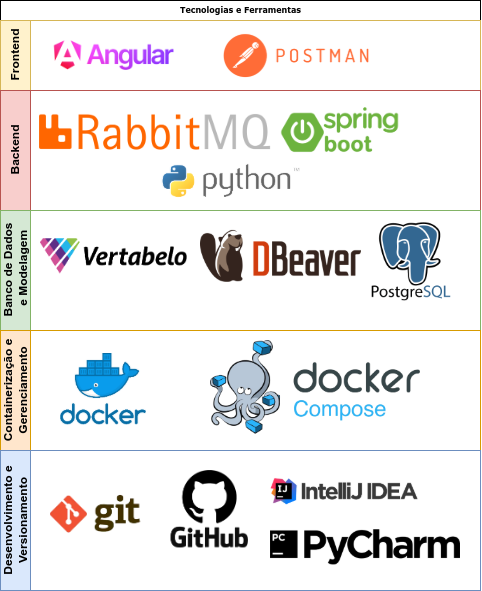
\includegraphics[scale=0.5]{imagens/sentilytics/diagramas/tecnologias-ferramentas.png}
\end{center}
}
\legend{Fonte: Autor (2025).}
\end{figure}

Na \autoref{diagrama_tecnologias_ferramentas}, a categorização das
tecnologias evidencia a variedade de ferramentas que compõem o
ecossistema do projeto. Cada categoria agrupa soluções com funções
específicas, demonstrando a pluralidade de abordagens utilizadas no
desenvolvimento. Com essa estrutura tecnológica bem definida, podemos
garantir um fluxo de trabalho mais eficiente e uma base sólida para a
implementação do sistema.

\hypertarget{python}{%
\subsection{Python}\label{python}}

O Python\footnote{O site do python está disponível no link:
  \url{https://www.python.org/}} é uma linguagem de programação
amplamente utilizada para tarefas de Processamento de Linguagem Natural
(PLN) devido à sua sintaxe acessível e ao amplo suporte de bibliotecas
voltadas para esse domínio. Entre os recursos disponíveis, destacam-se
ferramentas como o \emph{Natural Language Toolkit} (NLTK), que fornece
funcionalidades para tokenização, remoção de \emph{stopwords},
\emph{stemming} e lematização, e o Enelvo, uma biblioteca voltada para a
normalização de textos em português \cite{bertaglia2016exploring}. Essas
bibliotecas possibilitam a manipulação eficiente de textos, sendo
frequentemente aplicadas em soluções que envolvem análise automática de
conteúdos.

No desenvolvimento do Sentilytics, o Python foi utilizado para
implementar o serviço responsável pelo pré-processamento e pela análise
de sentimentos das postagens coletadas. Esse serviço é projetado para
funcionar de forma assíncrona e escalável, utilizando o RabbitMQ como
sistema de mensageria para gerenciar os processos. Dessa forma, é
possível processar grandes volumes de dados de maneira organizada.

O pré-processamento é iniciado quando o serviço recebe uma mensagem pelo
RabbitMQ, indicando que deve buscar na base de dados os textos brutos e
as tarefas de pré-processamento configuradas pelo usuário. Após essa
busca, o serviço aplica as tarefas selecionadas aos textos coletados.
Essas tarefas podem incluir:

\begin{itemize}
\tightlist
\item
  Remoção de stopwords: Eliminação de palavras irrelevantes para a
  análise, como ``de'', ``o'', ``para'';
\item
  Normalização e lematização: Ajuste dos textos para uniformidade e
  redução de palavras à sua forma base;
\item
  Correção ortográfica: Identificação e ajuste de erros ortográficos nos
  textos.
\end{itemize}

Essas etapas garantem que os dados sejam limpos e livres de ruídos,
tornando-os adequados para a análise de sentimentos. Após o término do
pré-processamento, o texto resultante é salvo na base de dados e uma
mensagem é enviada via RabbitMQ, notificando o término do processo.

A análise de sentimentos também é gerenciada por meio do RabbitMQ, que
envia uma mensagem para iniciar o processo. A partir dessa notificação,
o serviço recupera as postagens pré-processadas da base de dados e
aplica o modelo de análise de sentimentos VADER, fornecido pela
biblioteca NLTK. Esse modelo, por sua leveza e facilidade de
implementação, foi escolhido para esta versão do Sentilytics. Após a
análise, os resultados são armazenados na base de dados, e uma mensagem
é enviada pelo RabbitMQ informando o término do processo.

Embora atualmente apenas o VADER esteja integrado à solução, a
arquitetura do Sentilytics foi projetada para permitir futuras
expansões. Isso inclui a possibilidade de integrar novos modelos de
análise de sentimentos e oferecer ao usuário a opção de selecionar o
modelo desejado, da mesma forma como ocorre com a configuração das
tarefas de pré-processamento.

\hypertarget{spring-boot}{%
\subsection{Spring Boot}\label{spring-boot}}

O Spring Boot\footnote{A documentação do Spring Boot está disponível no
  link: \url{https://spring.io/projects/spring-boot}} é um
\emph{framework} Java voltado para o desenvolvimento de aplicações web e
serviços \emph{back-end}, oferecendo uma abordagem simplificada para a
configuração e execução de sistemas baseados no ecossistema Spring. Ele
possibilita a criação de aplicações modulares e escaláveis, reduzindo a
necessidade de configurações manuais extensivas e proporcionando
integração com diversas tecnologias, como bancos de dados, filas de
mensagens e processamento em lote.

Além do suporte para APIs REST, o Spring Boot conta com o Spring Batch,
uma extensão projetada para lidar com grandes volumes de dados por meio
de processamento assíncrono e em lote. Esse módulo é amplamente
utilizado em cenários que exigem a importação e transformação de grandes
conjuntos de informações de forma eficiente e estruturada.

No desenvolvimento do Sentilytics, o Spring Boot foi utilizado para
construir dois serviços principais, cada um desempenhando um papel
fundamental na arquitetura da aplicação:

\begin{enumerate}
\def\labelenumi{\arabic{enumi})}
\item
  Web API (Spring Boot REST API) -- Esse serviço atua como o núcleo de
  comunicação da aplicação, centralizando todas as operações e
  integrando os diferentes módulos do sistema. Ele expõe os endpoints
  REST que permitem a interação com o \emph{front-end} em Angular e
  gerencia a inicialização dos serviços oferecidos pelo módulo em
  Python, como o pré-processamento e a análise de sentimentos,
  utilizando o RabbitMQ para troca de mensagens. Além disso, a API é
  responsável pela coleta de dados no Bluesky, lidando com a
  autenticação necessária e garantindo a ingestão segura das postagens
  na base de dados PostgreSQL. A escolha do Bluesky como rede social
  integrada justifica-se pela política de gratuidade na coleta de
  postagens, o que viabilizou a realização deste estudo de caso. Apesar
  de o Bluesky ainda não ser amplamente utilizado no Brasil, sua
  estrutura e acessibilidade tornam-no uma escolha viável para a
  demonstração das funcionalidades do Sentilytics. A API também gerencia
  os workflows e coordena as operações realizadas dentro da plataforma,
  garantindo que cada requisição seja processada de maneira consistente;
\item
  Spring Batch -- A segunda aplicação desenvolvida com Spring Boot foi
  um serviço baseado no Spring Batch, utilizado para a importação e
  processamento de dados a partir de arquivos CSV. Esse recurso permite
  que os usuários superem a limitação atual de depender exclusivamente
  do Bluesky como fonte de dados, possibilitando a análise de qualquer
  conjunto de textos formatados em arquivos CSV. Dessa forma, a
  plataforma se torna mais versátil e capaz de atender a diferentes
  necessidades analíticas, independentemente da origem dos dados. O
  Spring Batch garante que a solução lide com grandes quantidades de
  postagens sem comprometer o desempenho da plataforma, validando e
  processando os dados de forma eficiente antes de armazená-los no banco
  de dados.
\end{enumerate}

A utilização do Spring Boot no projeto possibilitou uma estrutura
modular, escalável e organizada, facilitando a manutenção e a expansão
do sistema conforme novas funcionalidades forem incorporadas.

\hypertarget{angular}{%
\subsection{Angular}\label{angular}}

O Angular\footnote{A documentação do Angular está disponível no link:
  \url{https://angular.dev/}} é um \emph{framework} \emph{front-end}
baseado em TypeScript, desenvolvido e mantido pelo Google, voltado para
a criação de aplicações web dinâmicas e escaláveis. Ele adota uma
arquitetura modular baseada em componentes reutilizáveis, proporcionando
um desenvolvimento estruturado e facilitando a manutenção do código.

No desenvolvimento de interfaces, o Angular pode ser combinado com
bibliotecas de estilização como o Tailwind CSS, um \emph{framework} CSS
utilitário que permite a criação de layouts responsivos e altamente
customizáveis, reduzindo a necessidade de estilos manuais.

No desenvolvimento do Sentilytics, o Angular foi utilizado como o
\emph{framework} principal para construção do \emph{front-end}. Para
facilitar a estilização e responsividade, o \emph{framework} foi
utilizado em conjunto com o Tailwind CSS, que possibilitou a criação de
um design moderno e consistente sem a necessidade de escrever estilos
CSS extensos.

A interface foi projetada para proporcionar uma navegação intuitiva,
organizando as diferentes etapas do fluxo da aplicação, desde o cadastro
da pesquisa, passando pela coleta e processamento dos dados, até a
visualização dos resultados da análise de sentimentos.

Além disso, para garantir uma experiência em tempo real, foi
implementado o protocolo Server-Sent Events (SSE), que permite a
comunicação assíncrona entre o \emph{back-end} e o \emph{front-end}.
Esse mecanismo foi utilizado para notificar os usuários sobre o
andamento de processos demorados, como o pré-processamento dos textos e
a execução da análise de sentimentos. Dessa forma, os usuários podem
acompanhar o progresso das operações sem a necessidade de recarregar a
página ou realizar requisições manuais para obter atualizações.

\hypertarget{rabbitmq}{%
\subsection{RabbitMQ}\label{rabbitmq}}

O RabbitMQ\footnote{O RabbitMQ está disponível para download no link:
  \url{https://www.rabbitmq.com/}} é um sistema de mensageria de código
aberto utilizado para comunicação assíncrona entre serviços, permitindo
a troca de mensagens de forma eficiente e desacoplada. Ele funciona como
um intermediário que gerencia filas de mensagens, garantindo que os
componentes de um sistema possam se comunicar sem dependências diretas,
o que contribui para a escalabilidade e resiliência da aplicação.

O RabbitMQ opera por meio do modelo Produtor-Consumidor, onde mensagens
são publicadas em filas e processadas por serviços que as consomem
conforme sua disponibilidade. Essa abordagem permite a distribuição de
carga e melhora o desempenho em aplicações que lidam com grandes volumes
de processamento, evitando bloqueios e garantindo que as solicitações
sejam tratadas de forma ordenada.

Além disso, o RabbitMQ pode ser integrado a diferentes tecnologias,
oferecendo suporte para diversos protocolos e padrões de comunicação,
como AMQP (Advanced Message Queuing Protocol). Sua arquitetura permite o
gerenciamento de múltiplas filas e consumidores, otimizando o
processamento paralelo e a distribuição eficiente de tarefas.

O RabbitMQ foi utilizado como broker de mensagens para possibilitar a
comunicação assíncrona entre o serviço de pré-processamento e análise de
sentimentos em Python e a API REST desenvolvida em Spring Boot. Por meio
desse mecanismo, as requisições de processamento são enviadas para filas
de mensagens, permitindo que o sistema execute as operações de forma
desacoplada e escalável, sem a necessidade de bloqueios ou espera ativa.

\hypertarget{postgresql}{%
\subsection{PostgreSQL}\label{postgresql}}

O PostgreSQL\footnote{O PostgreSQL está disponível para download no
  link: \url{https://www.postgresql.org/}} é um sistema de gerenciamento
de banco de dados relacional (SGBD) de código aberto, reconhecido por
sua conformidade com padrões SQL e suporte a transações ACID
(Atomicidade, Consistência, Isolamento e Durabilidade). Ele oferece
mecanismos para garantir a integridade dos dados e eficiência na
execução de consultas.

Além de suas funcionalidades relacionais, o PostgreSQL permite o uso de
índices personalizados, replicação e extensões para aprimoramento do
desempenho e escalabilidade. Sua compatibilidade com diversas linguagens
e \emph{frameworks} possibilita a integração com diferentes tipos de
aplicações.

O PostgreSQL foi utilizado como o banco de dados relacional da
aplicação, armazenando informações essenciais como pesquisas, postagens
coletadas, workflows de processamento e resultados das análises de
sentimentos. Sendo a principal fonte de armazenamento de Sentilytics.

\hypertarget{git-e-github}{%
\subsection{Git e GitHub}\label{git-e-github}}

O Git\footnote{O Git está disponível para download no link:
  \url{https://git-scm.com/}} é um sistema de controle de versão
distribuído, amplamente utilizado para o gerenciamento de código-fonte
em projetos de software. Ele permite que desenvolvedores rastreiem
alterações no código, colaborem de forma eficiente e revertam
modificações sempre que necessário. O Git funciona por meio de
repositórios que armazenam diferentes versões dos arquivos, garantindo
organização e controle durante o ciclo de desenvolvimento.

O GitHub\footnote{O Github está disponível no link:
  \url{https://github.com/}} é uma plataforma baseada na web que fornece
um ambiente para hospedagem de repositórios Git. Além do armazenamento
de código, o GitHub oferece ferramentas para colaboração, gerenciamento
de projetos e automação de fluxos de trabalho.

No desenvolvimento do Sentilytics, o Git foi utilizado para
versionamento e controle das alterações nos diferentes projetos que
compõem a aplicação. Já o GitHub foi utilizado para armazenar os
repositórios e gerenciar o ciclo de desenvolvimento de forma
centralizada.

Além do controle de versão, o GitHub Actions foi empregado para
automatizar a geração e armazenamento de imagens Docker dos serviços do
sistema. Esse processo nas seguintes etapas:

\begin{enumerate}
\def\labelenumi{\arabic{enumi})}
\tightlist
\item
  Monitoramento de alterações -- Sempre que novas mudanças são enviadas
  para o repositório em uma branch especifica, um workflow do GitHub
  Actions é acionado automaticamente;
\item
  Geração da imagem Docker -- O código atualizado é processado para
  criar uma nova versão da imagem do serviço correspondente;
\item
  Armazenamento no GitHub Container Registry -- Após a construção da
  imagem, ela é enviada e armazenada no GitHub Container Registry,
  garantindo que os serviços estivessem sempre prontos para implantação.
\end{enumerate}

O uso do Git, GitHub e GitHub Actions possibilitou um fluxo contínuo de
integração (CI), facilitando a manutenção e a implantação do
Sentilytics.

\hypertarget{docker-e-docker-compose}{%
\subsection{Docker e Docker Compose}\label{docker-e-docker-compose}}

O Docker\footnote{Para saber mais sobre o Docker acesse o link:
  \url{https://www.docker.com/}} é uma plataforma que permite a criação,
distribuição e execução de containers, que são ambientes isolados que
contêm todas as dependências necessárias para a execução de uma
aplicação. Ao invés de instalar diretamente os serviços no sistema
operacional, o Docker encapsula tudo em imagens, garantindo
portabilidade, consistência e facilidade na implantação dos sistemas em
diferentes ambientes.

O Docker Compose\footnote{Você pode ler mais sobre o Docker Compose no
  link: \url{https://docs.docker.com/compose/}} é uma ferramenta
complementar ao Docker que permite a orquestração de múltiplos
containers de maneira simplificada. Ele utiliza um arquivo de
configuração no formato YAML para definir quais serviços devem ser
executados, suas interações e configurações específicas, permitindo a
inicialização conjunta de diferentes componentes de um sistema.

No desenvolvimento do Sentilytics, o Docker foi utilizado para criar
imagens Docker de todos os componentes do sistema, garantindo que cada
serviço fosse executado de forma isolada e sem dependências externas
diretas. Com isso, cada parte do sistema pôde ser facilmente distribuída
e implantada, independentemente do ambiente em que fosse executada.

Além disso, foi criado um Docker Compose de exemplo para facilitar a
orquestração e execução dos containers, permitindo que os serviços do
Sentilytics fossem iniciados de maneira unificada. Esse arquivo define
quais containers devem ser executados, estabelecendo as configurações
necessárias para a comunicação entre eles.

A utilização do Docker e Docker Compose no projeto trouxe benefícios
como padronização do ambiente de execução e facilidade na implantação,
garantindo que todos os serviços possam ser executados de forma
consistente em qualquer infraestrutura compatível com Docker.

\hypertarget{intellij-idea}{%
\subsection{Intellij IDEA}\label{intellij-idea}}

O IntelliJ IDEA\footnote{O Intellij IDEA está disponível para download
  no link: \url{https://www.jetbrains.com/idea/}} é um ambiente de
desenvolvimento integrado (IDE) voltado para a criação de aplicações em
Java e Kotlin. Desenvolvido pela JetBrains, oferece suporte a diversas
tecnologias e \emph{frameworks}, além de ferramentas de depuração e
controle de versão que auxiliam no processo de desenvolvimento.

A IDE conta com recursos como autocompletar código, análise estática e
refatoração, proporcionando um ambiente estruturado para a escrita e
manutenção de código. Sua compatibilidade com \emph{frameworks} como
Spring Boot e ferramentas de automação como Maven facilita a
configuração e o gerenciamento de projetos Java. O Intellij foi
utilizado em todos os projetos java desenvolvidos nessa solução.

\hypertarget{pycharm}{%
\subsection{PyCharm}\label{pycharm}}

O PyCharm\footnote{O Pycharm está disponível para download no link:
  \url{https://www.jetbrains.com/pycharm/}} é um ambiente de
desenvolvimento integrado (IDE) voltado para aplicações em Python,
desenvolvido pela JetBrains. Ele oferece suporte a \emph{frameworks} e
bibliotecas da linguagem, além de ferramentas de depuração, análise de
código e controle de versão.

A IDE conta com recursos como autocompletar de código, refatoração
automatizada e suporte a testes unitários, facilitando a escrita e
manutenção de código. No Sentilytics, o PyCharm foi utilizado como a IDE
principal para o desenvolvimento do serviço Python.

\hypertarget{visual-studio-code-vs-code}{%
\subsection{Visual Studio Code (VS
Code)}\label{visual-studio-code-vs-code}}

O Visual Studio Code (VS Code)\footnote{O VS Code está disponível para
  download no link: \url{https://code.visualstudio.com/}} é um editor de
código-fonte desenvolvido pela Microsoft, amplamente utilizado devido à
sua leveza, extensibilidade e suporte a diversas linguagens de
programação. Ele conta com recursos como realce de sintaxe, IntelliSense
(autocompletar inteligente) e integração com ferramentas externas,
facilitando o desenvolvimento e a depuração de código. Sendo o VS Code a
principal ferramenta para desenvolvimento do \emph{front-end} em
Angular.

\hypertarget{dbeaver}{%
\subsection{DBeaver}\label{dbeaver}}

O DBeaver\footnote{O DBeaver está disponível para download no link:
  \url{https://dbeaver.io/}} é uma ferramenta universal de administração
de bancos de dados, compatível com diversos sistemas de gerenciamento de
banco de dados (SGBDs), incluindo PostgreSQL, MySQL, SQL Server e
outros. Ele fornece uma interface gráfica para executar queries SQL,
visualizar e editar tabelas, além de gerenciar conexões com diferentes
bancos de dados.

A ferramenta também permite a exportação de dados em diferentes
formatos, facilitando a análise externa e a validação das informações
armazenadas. Além disso, oferece suporte a diversos recursos avançados,
como modelagem de dados, execução de scripts e monitoramento de
desempenho das consultas.

O DBeaver foi utilizado como ferramenta de administração do banco de
dados PostgreSQL, permitindo a execução de consultas SQL, visualização e
manipulação dos dados armazenados, facilitando o gerenciamento e a
validação das informações durante o desenvolvimento do Sentilytics.

\hypertarget{vertabelo}{%
\subsection{Vertabelo}\label{vertabelo}}

O Vertabelo\footnote{O Vertabelo está pode ser acessado no link:
  \url{https://my.vertabelo.com/}} é uma ferramenta online para
modelagem de bancos de dados, permitindo a criação de esquemas
relacionais de forma visual. Ele fornece suporte à modelagem
Entidade-Relacionamento (ER), facilitando a definição de tabelas, chaves
primárias e estrangeiras, além da geração automática do código SQL e
dicionário de dados correspondente.

A plataforma possibilita ajustes no modelo sem a necessidade de
instalação de software adicional. Ainda mais, a plataforma oferece a
exportação de diagramas para diferentes formatos, auxiliando na
documentação e na comunicação entre equipes de desenvolvimento.

O Vertabelo foi utilizado para a modelagem do banco de dados, permitindo
a criação do Diagrama Entidade-Relacionamento (DER) e a geração do
Dicionário de Dados. Essa ferramenta facilitou a estruturação das
tabelas e seus relacionamentos no PostgreSQL, auxiliando no planejamento
e na organização dos dados do Sentilytics, garantindo uma base bem
documentada.

\hypertarget{postman}{%
\subsection{Postman}\label{postman}}

O Postman\footnote{O postman está disponível para download no link:
  \url{https://www.postman.com/}} é uma ferramenta utilizada para
desenvolvimento, teste e documentação de APIs, permitindo a realização
de requisições HTTP de maneira prática. Ele suporta diferentes métodos
de requisição, como GET, POST, PUT e DELETE, possibilitando a
verificação do funcionamento dos endpoints e a validação das respostas
retornadas pelo servidor.

A ferramenta também permite a visualização de dados em formatos como
JSON e XML, além de oferecer recursos para organização de coleções de
requisições e automação de testes. Outra funcionalidade relevante é o
gerenciamento de variáveis de ambiente, facilitando a adaptação de
requisições para diferentes contextos, como desenvolvimento e produção.

O Postman foi utilizado para testar e validar todas as APIs
desenvolvidas no Sentilytics, incluindo a API REST em Spring Boot e as
integrações com o Bluesky. A ferramenta permitiu a realização de
requisições HTTP, validando o funcionamento do serviços criados no
\emph{back-end} e facilitando a depuração durante o desenvolvimento.

Finalizada a apresentação das tecnologias e ferramentas, seguimos agora
para a próxima etapa, onde abordaremos a modelagem da solução.

\hypertarget{modelagem-da-soluuxe7uxe3o}{%
\section{Modelagem da solução}\label{modelagem-da-soluuxe7uxe3o}}

A modelagem da solução é uma etapa fundamental no desenvolvimento de
sistemas, pois permite a representação visual e descritiva dos
componentes, fluxos de dados e interações entre os elementos da
aplicação. Através dessa modelagem, é possível compreender a estrutura
da solução proposta, identificar os requisitos essenciais e garantir que
a implementação esteja alinhada com os objetivos do projeto.

A aplicação desenvolvida para análise de sentimentos em redes sociais
exige uma modelagem robusta que aborde tanto os aspectos funcionais
quanto os estruturais do sistema. Para isso, são utilizados diferentes
diagramas e especificações, que descrevem desde os requisitos funcionais
e não funcionais até a arquitetura dos componentes e o fluxo de
processamento dos dados.

Inicialmente, são definidos os requisitos funcionais e não funcionais,
que estabelecem as funcionalidades esperadas e as restrições técnicas da
aplicação. Em seguida, o Diagrama de Caso de Uso apresenta as principais
interações entre os usuários e o sistema, facilitando a compreensão das
funcionalidades disponíveis.

Para representar o fluxo de execução dos processos dentro da aplicação,
são utilizados diagramas BPMN (Business Process Model and Notation) e
diagramas de sequência/atividades, que detalham as etapas do
pré-processamento e da análise de sentimentos. Além disso, a estrutura
de dados e as relações entre entidades são documentadas por meio do
Diagrama Entidade-Relacionamento (DER) e do dicionário de dados.

A organização dos componentes do sistema é descrita no Diagrama de
Componentes, que ilustra a arquitetura da aplicação, destacando a
comunicação entre os módulos do \emph{back-end}, \emph{front-end} e
serviços externos. Complementarmente, o Diagrama de Classes define a
estrutura da lógica de programação, detalhando as principais classes e
seus relacionamentos.

Por fim, as interfaces gráficas são apresentadas para demonstrar a
experiência do usuário e a forma como as funcionalidades da aplicação
são disponibilizadas. Essas interfaces são projetadas para garantir
usabilidade, responsividade e uma experiência intuitiva, permitindo que
os usuários explorem as análises de sentimentos de maneira eficiente.

Com essa modelagem, busca-se garantir que a aplicação seja bem
estruturada, escalável e de fácil manutenção, possibilitando futuras
melhorias e adaptações conforme novas necessidades forem identificadas.

\hypertarget{requisitos-funcionais-e-nuxe3o-funcionais}{%
\subsection{Requisitos Funcionais e Não
Funcionais}\label{requisitos-funcionais-e-nuxe3o-funcionais}}

Para garantir que a aplicação de análise de sentimentos em redes sociais
atenda aos objetivos propostos, é essencial definir os requisitos
funcionais e não funcionais. Os requisitos funcionais descrevem as
funcionalidades que o sistema deve oferecer, especificando as interações
entre usuários e a aplicação. Já os requisitos não funcionais
estabelecem critérios de qualidade, desempenho, segurança e usabilidade.
O \autoref{requisitos_funcionais} apresenta os principais requisitos
funcionais que orientaram o desenvolvimento da solução proposta.

\renewcommand\LTcaptype{quadro}
\begin{longtable}[]{|c|l|}
\caption{Requisitos funcionais.\label{requisitos_funcionais}}\tabularnewline
\toprule
\begin{minipage}[b]{0.07\columnwidth}\centering
Código\strut
\end{minipage} & \begin{minipage}[b]{0.87\columnwidth}\raggedright
Requisito\strut
\end{minipage}\tabularnewline
\midrule
\endhead
\begin{minipage}[t]{0.07\columnwidth}\centering
RF01\strut
\end{minipage} & \begin{minipage}[t]{0.87\columnwidth}\raggedright
O sistema deve permitir a coleta de postagens da rede social Bluesky, respeitando parâmetros de data inicial, data final, query de busca e linguagem.\strut
\end{minipage}\tabularnewline
\begin{minipage}[t]{0.07\columnwidth}\centering
RF02\strut
\end{minipage} & \begin{minipage}[t]{0.87\columnwidth}\raggedright
O sistema deve permitir como forma alternativa a importação de postagens no formato CSV para análise de sentimentos, utilizando Spring Batch para processamento da importação.\strut
\end{minipage}\tabularnewline
\begin{minipage}[t]{0.07\columnwidth}\centering
RF03\strut
\end{minipage} & \begin{minipage}[t]{0.87\columnwidth}\raggedright
O sistema deve permitir que o usuário configure workflows e escolha quais tarefas de pré-processamento serão aplicadas aos dados coletados.\strut
\end{minipage}\tabularnewline
\begin{minipage}[t]{0.07\columnwidth}\centering
RF04\strut
\end{minipage} & \begin{minipage}[t]{0.87\columnwidth}\raggedright
O sistema deve possibilitar a limpeza e normalização dos textos coletados, incluindo remoção de stopwords, lematização e tokenização.\strut
\end{minipage}\tabularnewline
\begin{minipage}[t]{0.07\columnwidth}\centering
RF05\strut
\end{minipage} & \begin{minipage}[t]{0.87\columnwidth}\raggedright
O sistema deve calcular a pontuação de sentimentos de cada comentário, classificando-os como positivos, negativos ou neutros com base em regras de pontuação composta.\strut
\end{minipage}\tabularnewline
\begin{minipage}[t]{0.07\columnwidth}\centering
RF06\strut
\end{minipage} & \begin{minipage}[t]{0.87\columnwidth}\raggedright
O sistema deve armazenar os resultados da análise de sentimentos em uma tabela de banco de dados, incluindo a quantidade total de comentários e a distribuição de sentimentos.\strut
\end{minipage}\tabularnewline
\begin{minipage}[t]{0.07\columnwidth}\centering
RF07\strut
\end{minipage} & \begin{minipage}[t]{0.87\columnwidth}\raggedright
O sistema deve permitir a consulta dos resultados da análise de sentimentos, filtrando por período, rede social e sentimento predominante.\strut
\end{minipage}\tabularnewline
\begin{minipage}[t]{0.07\columnwidth}\centering
RF08\strut
\end{minipage} & \begin{minipage}[t]{0.87\columnwidth}\raggedright
O sistema deve permitir a comunicação entre o \emph{back-end} em Spring Boot e o serviço de análise de sentimentos em Python por meio de RabbitMQ.\strut
\end{minipage}\tabularnewline
\begin{minipage}[t]{0.07\columnwidth}\centering
RF09\strut
\end{minipage} & \begin{minipage}[t]{0.87\columnwidth}\raggedright
O sistema deve permitir que usuários se autentiquem utilizando suas credenciais da rede social Bluesky, sem a necessidade de cadastro adicional.\strut
\end{minipage}\tabularnewline
\begin{minipage}[t]{0.07\columnwidth}\centering
RF10\strut
\end{minipage} & \begin{minipage}[t]{0.87\columnwidth}\raggedright
O sistema deve fornecer uma interface web baseada em Angular para que os usuários possam interagir com as funcionalidades de análise de sentimentos.\strut
\end{minipage}\tabularnewline
\bottomrule
\caption*{Fonte: Autor (2025).}
\end{longtable}
\renewcommand\LTcaptype{table}

Com os requisitos funcionais definidos como mostrado no
\autoref{requisitos_funcionais}, podemos visualizar como os usuários
interagem com o sistema e quais as funcionalidades deveram estar
disponíveis. Para isso, vamos utilizar o diagrama de casos de uso.

\hypertarget{diagramas-de-caso-de-uso}{%
\subsection{Diagramas de Caso de Uso}\label{diagramas-de-caso-de-uso}}

Os diagramas de caso de uso são representações gráficas que demonstram
as interações entre os usuários e um sistema, destacando as principais
funcionalidades disponíveis. Seu objetivo é ilustrar, de forma simples,
como os diferentes atores interagem com o sistema em cenários
específicos, auxiliando na compreensão dos requisitos e no planejamento
da aplicação. A seguir, apresenta-se um caso de uso relevante do
Sentilytics.

\begin{figure}[htbp]
\hypertarget{usecase}{%
\caption{Diagrama de Casos de Uso do Sentilytics}\label{usecase}
\begin{center}
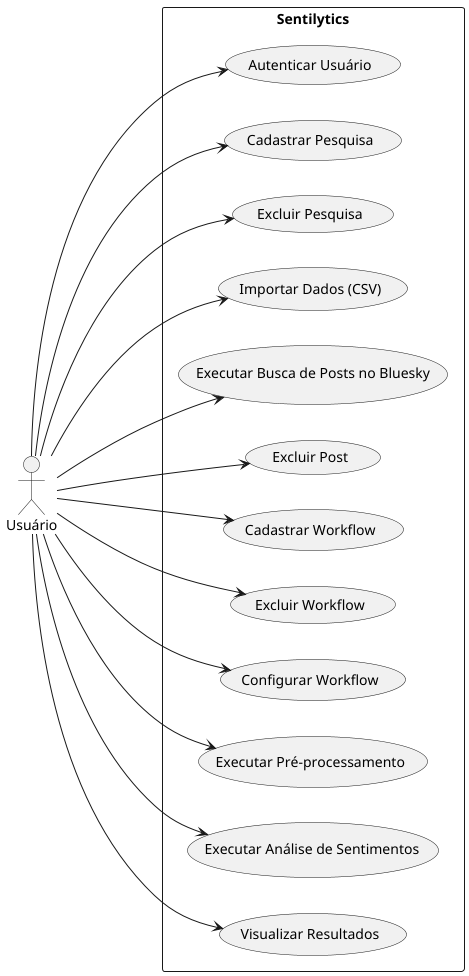
\includegraphics[scale=0.3]{imagens/sentilytics/diagramas/usecase.png}
\end{center}
}
\legend{Fonte: Autor (2025).}
\end{figure}

Como podemos visualizar na \autoref{usecase}, o diagrama apresenta as
interações entre o usuário e o sistema Sentilytics, destacando as
principais funcionalidades disponíveis. Cada caso de uso representa uma
ação que pode ser realizada dentro da aplicação, organizando de forma
clara os processos fundamentais do sistema.

O usuário pode realizar operações relacionadas à gestão de pesquisas,
como cadastrar, excluir e importar postagens diretamente via CSV e
realizar a busca de postagens na plataforma Bluesky. Também há
funcionalidades voltadas para a administração de workflows, permitindo o
cadastro, configuração das tarefas de pré-processamento e seus
parâmetros e exclusão desses componentes, que são essenciais para a
organização do processamento das postagens.

Ademais, o diagrama evidencia os processos de pré-processamento e
análise de sentimentos, que representam etapas centrais para obtenção
dos resultados. Após a execução do pré-processamento das postagens e em
seguida a análise do sentimentos, o usuário pode visualizar os
resultados gerados para aquele workflow processado, facilitando a
interpretação e análise das informações processadas pelo Sentilytics.

Com o diagrama de casos de uso definido, foi criada a modelagem do
principal processo da aplicação para estabelecer quais passos o usuário
deve seguir para criar uma pesquisa de análise de sentimentos.

\hypertarget{bpmn}{%
\subsection{BPMN}\label{bpmn}}

A Business Process Model and Notation (BPMN) é uma notação padronizada
para modelagem de processos de negócios, utilizada para representar o
fluxo de atividades dentro de um sistema ou organização. Seu propósito é
fornecer uma visão clara das etapas envolvidas em um processo,
facilitando sua análise e compreensão. A seguir, apresenta-se um
diagrama BPMN relacionado ao funcionamento do Sentilytics.

\begin{figure}[htbp]
\hypertarget{bpmn_pesquisa}{%
\caption{Modelagem BPMN do Processo de Pesquisa no Sentilytics}\label{bpmn_pesquisa}
\begin{center}
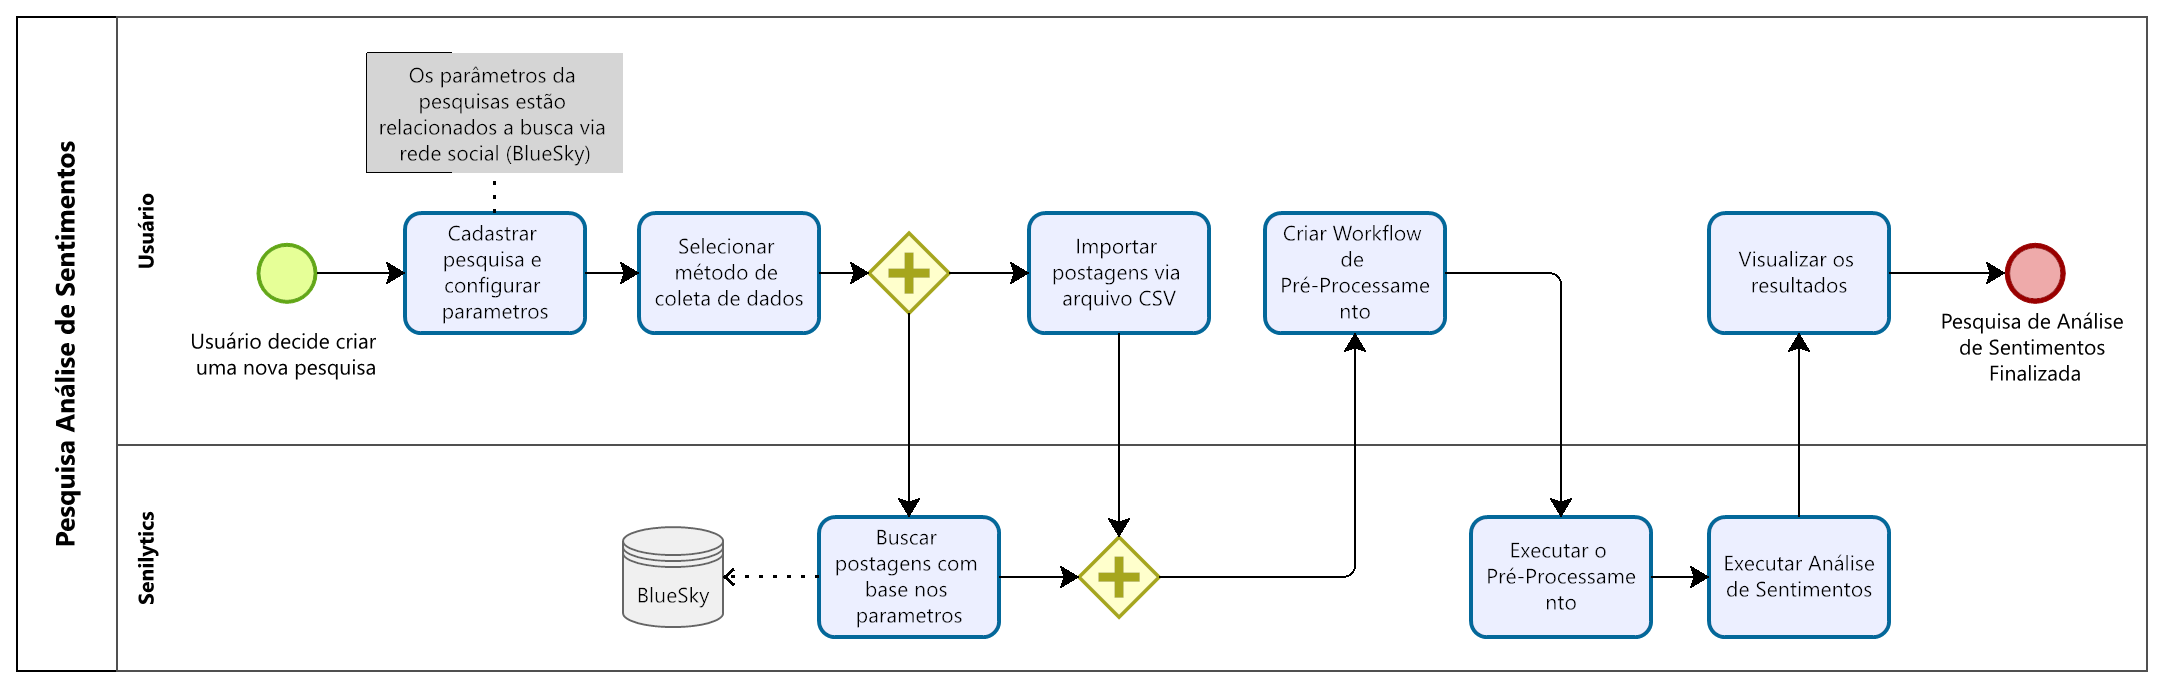
\includegraphics[scale=0.3]{imagens/sentilytics/pesquisa_sentimentos.png}
\end{center}
}
\legend{Fonte: Autor (2025).}
\end{figure}

A \autoref{bpmn_pesquisa} apresenta o fluxo principal para a realização
de uma pesquisa completa no Sentilytics, representado por meio do
Diagrama BPMN. Esse fluxo descreve as etapas envolvidas desde a criação
da pesquisa até a visualização dos resultados da análise de sentimentos.

O processo inicia-se quando o usuário decide realizar uma nova pesquisa,
cadastrando-a e configurando os parâmetros necessários. Em seguida, é
necessário definir o método de coleta de dados , onde duas abordagens
podem ser utilizadas de forma independente ou simultânea: importação de
dados via arquivo CSV ou a busca automatizada de postagens na plataforma
Bluesky .

Após a coleta dos dados, o próximo passo envolve a criação de um
workflow, que organiza o processamento dos textos coletados. O usuário,
então, inicia a fase de pré-processamento, na qual o sistema aplica as
tarefas configuradas no workflow pelo usuário, preparando os dados para
a análise.

Com os dados pré-processados, o usuário pode acionar a análise de
sentimentos naquele workflow já pré-processado, permitindo que o sistema
classifique os textos e gere os resultados. Após a execução desse
processamento, os resultados são disponibilizados para visualização,
possibilitando a interpretação dos dados analisados.

Vale notar que o usuário está livre para cadastrar diversos workflows,
cada um com suas particularidades na configuração, possuindo diferentes
tarefas de pré-processamento e parâmetros. Por fim, o fluxo se encerra
quando o usuário finaliza a pesquisa, consolidando os resultados
obtidos.

Com o processo definido, foi necessário estruturar a modelagem dos
dados. Para isso, foi elaborado o Diagrama Entidade-Relacionamento
(DER), que representa a estrutura do banco de dados e suas interações
com os elementos do sistema. Além disso, foi desenvolvido um dicionário
de dados para detalhar cada entidade e sua finalidade dentro da
aplicação.

\hypertarget{diagrama-entidade-relacionamento-der-e-dicionuxe1rio-de-dados}{%
\subsection{Diagrama Entidade-Relacionamento (DER) e Dicionário de
dados}\label{diagrama-entidade-relacionamento-der-e-dicionuxe1rio-de-dados}}

O Diagrama Entidade-Relacionamento (DER) é uma representação visual da
estrutura do banco de dados, destacando as entidades, seus atributos e
os relacionamentos entre elas. Ele permite compreender a organização dos
dados e a forma como as informações são armazenadas e manipuladas dentro
do sistema. No Sentilytics, o DER foi desenvolvido utilizando a
ferramenta Vertabelo, garantindo uma modelagem estruturada e alinhada
com os requisitos do sistema.

\begin{figure}[htbp]
\hypertarget{der}{%
\caption{Diagrama Entidade Relacionamento}\label{der}
\begin{center}
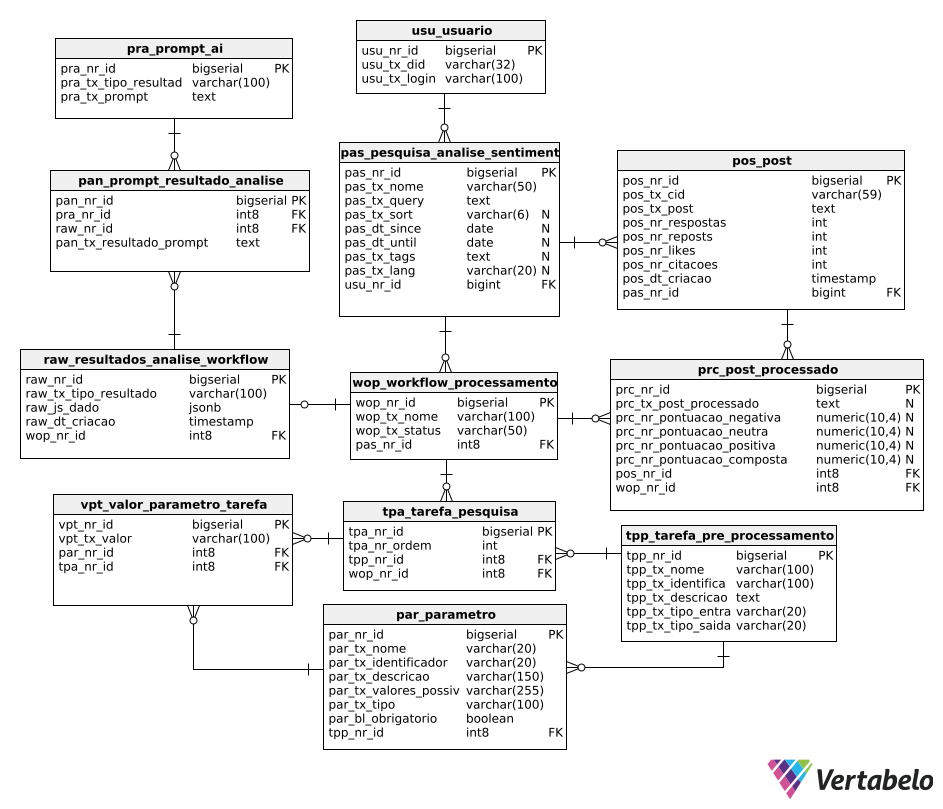
\includegraphics[scale=0.5]{imagens/sentilytics/diagramas/DER-sentilytics.png}
\end{center}
}
\legend{Fonte: Autor (2025).}
\end{figure}

A \autoref{der} apresenta o Diagrama Entidade-Relacionamento,
demonstrando a estrutura do banco de dados da aplicação. A modelagem foi
desenvolvida com base nos requisitos funcionais e processos definidos,
garantindo que a estrutura de dados suporte corretamente as
funcionalidades do sistema.

Complementando essa modelagem, o Dicionário de Dados fornece uma
descrição detalhada das tabelas, colunas, tipos de dados e restrições
aplicadas, servindo como uma referência essencial para o desenvolvimento
e manutenção do banco de dados. Esse recurso documenta a estrutura do
banco de forma organizada, facilitando a compreensão da modelagem e
assegurando a consistência dos dados ao longo do ciclo de vida da
aplicação.

\begin{figure}[htbp]
\hypertarget{dicionario_dados}{%
\caption{Dicionário de Dados}\label{dicionario_dados}
\begin{center}
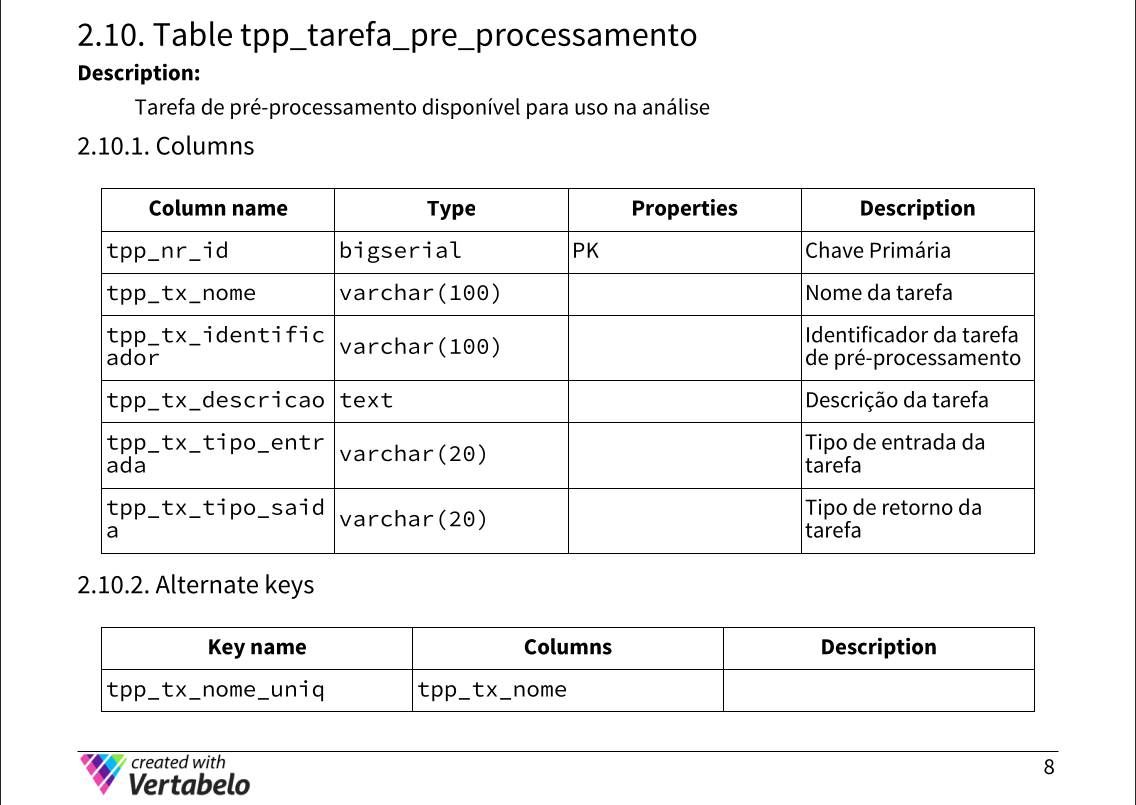
\includegraphics[scale=0.3]{imagens/sentilytics/diagramas/dicionario_dados.png}
\end{center}
}
\legend{Fonte: Autor (2025).}
\end{figure}

Assim como o DER, o Dicionário de Dados do Sentilytics foi gerado na
ferramenta Vertabelo, que permite a exportação e documentação
estruturada dos elementos do banco. A \autoref{dicionario_dados}
apresenta esse documento, refletindo a modelagem realizada e
consolidando a documentação do banco de dados. Após a modelagem da base
de dados, foi possível avançar com os diagramas de sequência/atividade
dos principais fluxos que foram mostrados nos requisitos.

\hypertarget{diagrama-de-sequuxeancia-do-pruxe9-processamento-e-anuxe1lise-de-sentimentos}{%
\subsection{Diagrama de Sequência do pré-processamento e análise de
sentimentos}\label{diagrama-de-sequuxeancia-do-pruxe9-processamento-e-anuxe1lise-de-sentimentos}}

Os diagramas de sequência são utilizados para representar a interação
entre diferentes componentes de um sistema ao longo do tempo. Eles
detalham a ordem das mensagens trocadas entre os elementos envolvidos,
permitindo a visualização do fluxo de execução de um processo
específico. Essa abordagem facilita a compreensão da dinâmica do sistema
e auxilia na identificação de dependências entre os componentes.

No contexto do Sentilytics, foram elaborados três diagramas de sequência
que descrevem processos essenciais para o funcionamento da aplicação:

\begin{itemize}
\tightlist
\item
  \autoref{seq_pesquisa_coleta_dados}: Cadastro da pesquisa e coleta de
  dados;
\item
  \autoref{seq_cadastro_configuracao_workflow}: Cadastro e configuração
  do workflow;
\item
  \autoref{seq_processamento_analise}: Sequência de processamento,
  incluindo o pré-processamento do workflow e da análise de sentimentos.
\end{itemize}

Cada um desses diagramas detalha a troca de informações entre os
elementos do sistema, evidenciando os passos necessários para a execução
dessas funcionalidades. A seguir, apresentam-se essas representações
gráficas.

\begin{figure}[htbp]
\hypertarget{seq_pesquisa_coleta_dados}{%
\caption{Diagrama de sequência do cadastro da pesquisa e coleta de dados}\label{seq_pesquisa_coleta_dados}
\begin{center}
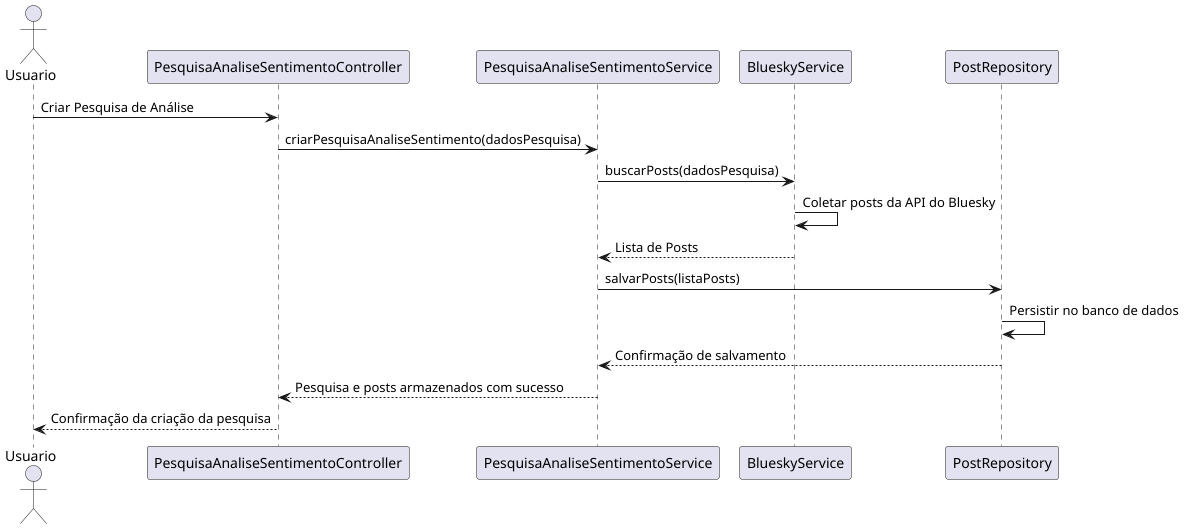
\includegraphics[scale=0.4]{imagens/sentilytics/diagramas/sequencia-cadastro-pesquisa-coleta-dados.png}
\end{center}
}
\legend{Fonte: Autor (2025).}
\end{figure}

A \autoref{seq_pesquisa_coleta_dados} apresenta o Diagrama de Sequência
que descreve o fluxo de criação de uma pesquisa de análise de
sentimentos e a coleta de dados a partir da plataforma Bluesky. Esse
diagrama detalha a interação entre o usuário e os principais componentes
do sistema durante esse processo.

O fluxo se inicia quando o usuário solicita a criação de uma nova
pesquisa. Essa requisição é recebida pelo
PesquisaAnaliseSentimentoController, que encaminha os dados para o
PesquisaAnaliseSentimentoService, responsável pelo gerenciamento da
lógica de negócio associada à pesquisa.

Em seguida, o serviço aciona o BlueskyService, que realiza a busca de
postagens na API do Bluesky com base nos parâmetros definidos na
pesquisa. Os dados coletados são então enviados de volta ao serviço
principal, que procede ao armazenamento das postagens. Para isso, a
lista de postagens é encaminhada ao PostRepository, que realiza a
persistência das informações no banco de dados.

Após a conclusão do armazenamento, o PostRepository confirma a operação,
retornando uma notificação ao PesquisaAnaliseSentimentoService. O
serviço, por sua vez, informa ao controller que a pesquisa e os posts
foram armazenados com sucesso. Por fim, o usuário recebe uma confirmação
da criação da pesquisa, sinalizando que o processo foi concluído
corretamente.

Esse diagrama ilustra de forma clara a sequência de interações entre os
componentes do sistema, destacando como a pesquisa é cadastrada e os
dados são coletados e armazenados para posterior análise.

\begin{figure}[htbp]
\hypertarget{seq_cadastro_configuracao_workflow}{%
\caption{Diagrama de sequência do cadastro e configuração do workflow}\label{seq_cadastro_configuracao_workflow}
\begin{center}
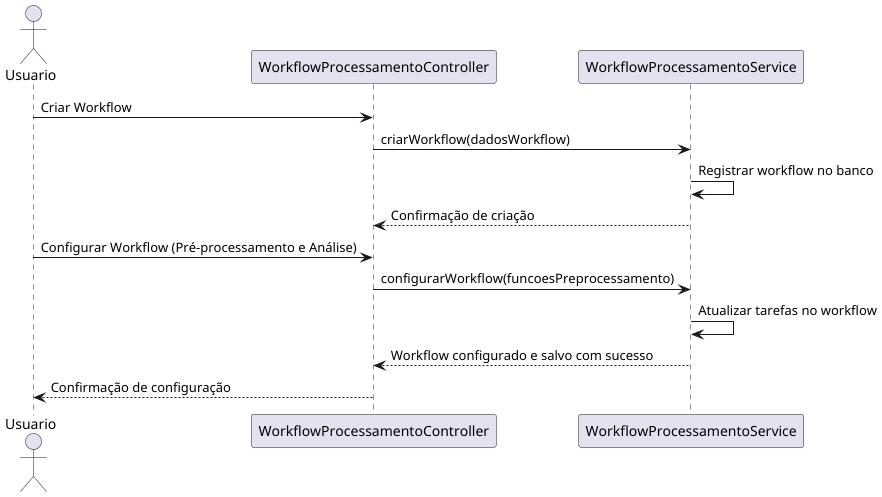
\includegraphics[scale=0.4]{imagens/sentilytics/diagramas/sequencia-cadastro-configuracao-workflow.png}
\end{center}
}
\legend{Fonte: Autor (2025).}
\end{figure}

A \autoref{seq_cadastro_configuracao_workflow} apresenta o Diagrama de
Sequência referente ao processo de cadastro e configuração do workflow
dentro do Sentilytics. Esse diagrama descreve a interação entre o
usuário e os principais componentes responsáveis pelo gerenciamento dos
workflows de processamento de dados.

O fluxo se inicia quando o usuário solicita a criação de um novo
workflow. Essa requisição é encaminhada ao
WorkflowProcessamentoController, que repassa os dados ao
WorkflowProcessamentoService, responsável por registrar o workflow no
banco de dados. Após a conclusão dessa etapa, uma confirmação de criação
é enviada ao usuário.

Após o cadastro, o usuário pode prosseguir com a configuração do
workflow, definindo as funções de pré-processamento e análise de
sentimentos que serão aplicadas aos dados coletados. Essa configuração
permite que o usuário ordene e selecione diferentes tarefas de
pré-processamento, como capitalização de texto, conversão para caixa
baixa, remoção de stopwords, correção ortográfica, entre outras. A ordem
dessas tarefas é um fator determinante para o processamento, pois
impacta diretamente os resultados da análise de sentimentos.

Quando o usuário finaliza a configuração, o
WorkflowProcessamentoController encaminha os dados ao
WorkflowProcessamentoService, que atualiza as informações do workflow no
banco de dados. Após essa operação, uma confirmação é enviada ao
usuário, indicando que o workflow foi configurado e salvo com sucesso.

Esse diagrama demonstra a estrutura do processo de cadastro e
configuração do workflow, garantindo que o sistema ofereça flexibilidade
na definição das etapas de processamento. Dessa forma, os usuários podem
ajustar o fluxo de análise de acordo com suas necessidades específicas.

\begin{figure}[htbp]
\hypertarget{seq_processamento_analise}{%
\caption{Diagrama de sequência do pré-processamento e análise}\label{seq_processamento_analise}
\begin{center}
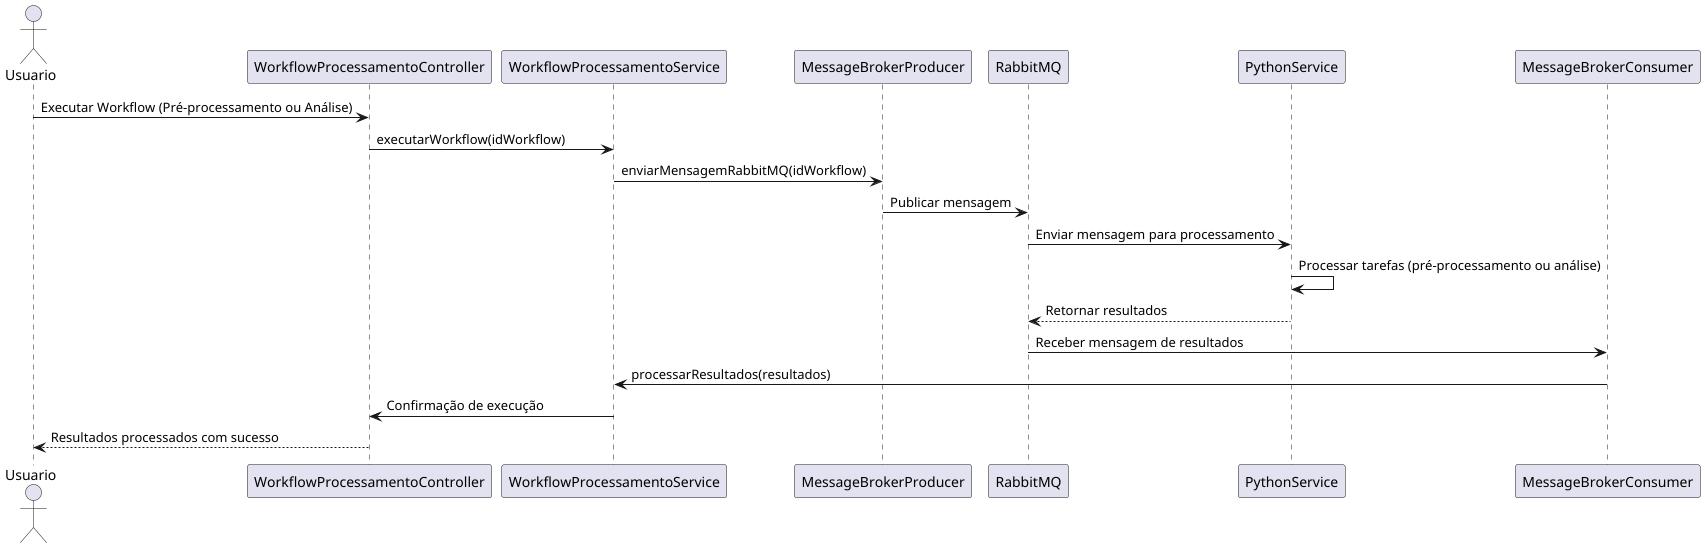
\includegraphics[scale=0.2]{imagens/sentilytics/diagramas/sequencia-pre-processamento-analise-sentimentos.png}
\end{center}
}
\legend{Fonte: Autor (2025).}
\end{figure}

A \autoref{seq_processamento_analise} apresenta o Diagrama de Sequência
que descreve o fluxo de execução de um workflow de processamento, que
representa o fluxo utilizado tanto para o pré-processamento do texto
quanto para a análise de sentimentos dentro do Sentilytics. Esse
diagrama detalha a interação entre o usuário e os serviços responsáveis
pelo envio, processamento e retorno dos dados.

O fluxo inicia-se quando o usuário solicita a execução de um workflow.
Essa requisição é encaminhada ao WorkflowProcessamentoController, que
direciona o processamento ao WorkflowProcessamentoService, responsável
por gerenciar a execução. Para iniciar o processamento, o serviço
encaminha a solicitação ao MessageBrokerProducer, que publica uma
mensagem na fila do RabbitMQ contendo a identificação do workflow a ser
processado.

O RabbitMQ então encaminha essa mensagem ao PythonService, que é
responsável por executar as tarefas associadas ao workflow. Dependendo
do tipo de processamento solicitado, esse serviço pode realizar etapas
de pré-processamento, como remoção de stopwords, normalização e correção
ortográfica, ou realizar a análise de sentimentos, atribuindo
classificações às postagens processadas.

Após a conclusão do processamento, o PythonService retorna os resultados
ao RabbitMQ, que os repassa ao MessageBrokerConsumer. O consumidor,
então, encaminha os resultados ao WorkflowProcessamentoService, que
processa e armazena as informações conforme necessário. Uma vez
finalizada essa etapa, o controller notifica o usuário informando que os
resultados foram processados com sucesso.

Esse diagrama destaca a estrutura assíncrona e desacoplada do
processamento dentro do Sentilytics, garantindo que tanto o
pré-processamento quanto a análise de sentimentos sejam executados de
maneira escalável. O uso do RabbitMQ como intermediário permite que as
solicitações sejam distribuídas e processadas conforme a capacidade do
sistema, evitando sobrecargas e garantindo a confiabilidade das
execuções.

\hypertarget{diagrama-de-classe}{%
\subsection{Diagrama de Classe}\label{diagrama-de-classe}}

O Diagrama de Classes é uma representação da estrutura estática do
sistema, demonstrando as classes que o compõem, seus atributos, métodos
e os relacionamentos entre elas. Esse modelo auxilia na compreensão da
arquitetura do sistema, permitindo uma visão clara da organização do
código e da interação entre os componentes.

Devido à complexidade da aplicação e à quantidade de classes envolvidas,
o diagrama de classes foi dividido em cinco partes, cada uma focada em
um pacote específico da Web API desenvolvida em Spring Boot. Essa
divisão facilita a análise dos diferentes níveis da aplicação,
proporcionando uma visão mais segmentada e compreensível.

Os diagramas são organizados da seguinte forma:

\begin{itemize}
\tightlist
\item
  Visão Geral dos Pacotes: Exibe a estrutura principal da aplicação,
  destacando os pacotes e suas respectivas classes;
\item
  Pacote Model: Representa as entidades do domínio, definindo os objetos
  que compõem o modelo de dados e seus relacionamentos;
\item
  Pacote Repository: Demonstra os repositórios responsáveis pela
  persistência dos dados, conectando a aplicação ao banco de dados;
\item
  Pacote Service: Contém as classes que implementam a lógica de negócio,
  garantindo o processamento e a manipulação dos dados conforme as
  regras da aplicação;
\item
  Pacote Controller: Representa os controladores da API, responsáveis
  por expor os endpoints e intermediar a comunicação entre o
  \emph{front-end} e a lógica de negócio.
\end{itemize}

A seguir, cada diagrama será apresentado e analisado individualmente,
detalhando a estrutura e os relacionamentos das classes dentro de cada
camada do sistema.

\begin{figure}[htbp]
\hypertarget{diagrama_classe_geral}{%
\caption{Diagrama de classes com visão geral dos pacotes}\label{diagrama_classe_geral}
\begin{center}
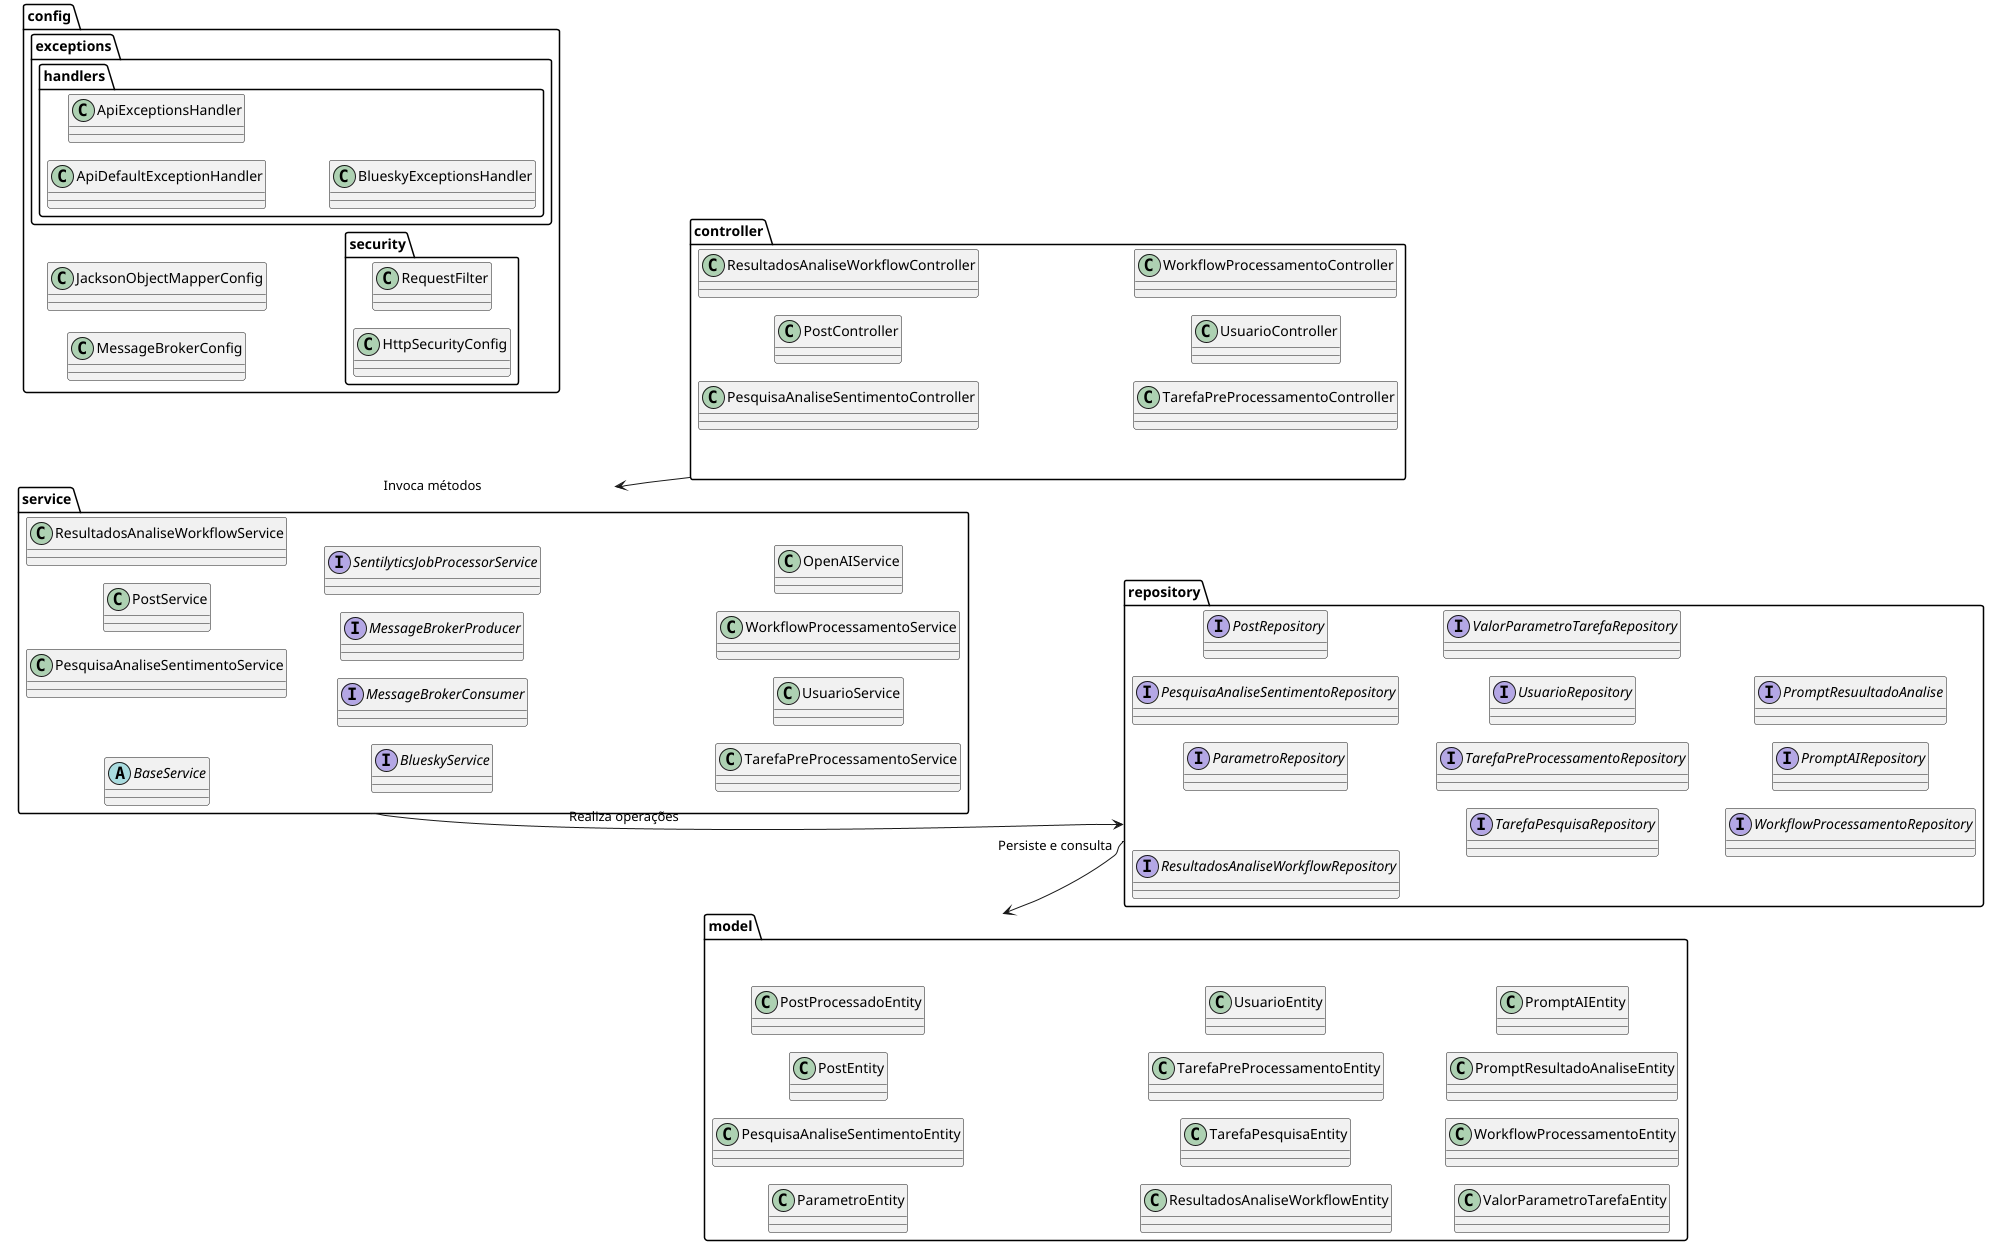
\includegraphics[scale=0.2]{imagens/sentilytics/diagramas/classes/diagrama-classe-visao-geral-pacotes.png}
\end{center}
}
\legend{Fonte: Autor (2025).}
\end{figure}

A \autoref{diagrama_classe_geral} apresenta a visão geral dos pacotes da
Web API desenvolvida em Spring Boot, destacando sua estrutura modular e
a organização das classes. Esse diagrama ilustra a separação dos
componentes do sistema, facilitando a compreensão das responsabilidades
de cada pacote e a interação entre eles.

A arquitetura segue uma estrutura organizada em camadas, conforme
descrito a seguir:

\begin{itemize}
\tightlist
\item
  Pacote controller: Contém as classes responsáveis por expor os
  endpoints da API, intermediando a comunicação entre o \emph{front-end}
  e a lógica de negócio da aplicação. Cada classe representa um
  controlador correspondente a um serviço específico;
\item
  Pacote service: Implementa a lógica de negócio do sistema, processando
  dados e aplicando as regras definidas. Essa camada interage
  diretamente com os repositórios para manipulação dos dados e com a
  camada de controle para fornecer respostas às requisições;
\item
  Pacote repository: Define os repositórios da aplicação, responsáveis
  pelo acesso e manipulação dos dados no banco de dados. As interfaces
  dessa camada utilizam o Spring Data JPA para abstrair operações de
  persistência;
\item
  Pacote model: Contém as entidades do domínio, que representam as
  tabelas do banco de dados e seus relacionamentos. Essa camada define a
  estrutura dos dados utilizados na aplicação;
\item
  Pacote config: Reúne configurações essenciais da aplicação, incluindo
  segurança, serialização e tratamento de exceções.
\end{itemize}

A comunicação entre os pacotes ocorre de forma estruturada: a camada de
controle interage com os serviços, que, por sua vez, realizam operações
no banco de dados por meio dos repositórios. O pacote de model é
utilizado pelos repositórios para representar os dados persistidos,
garantindo uma separação clara das responsabilidades dentro da
aplicação.

A seguir, será apresentada uma análise detalhada do Diagrama do Pacote
Model, que contém as entidades responsáveis pelo armazenamento e
manipulação dos dados no sistema.

\begin{figure}[htbp]
\hypertarget{diagrama_classe_model}{%
\caption{Diagrama de classes da camada Model}\label{diagrama_classe_model}
\begin{center}
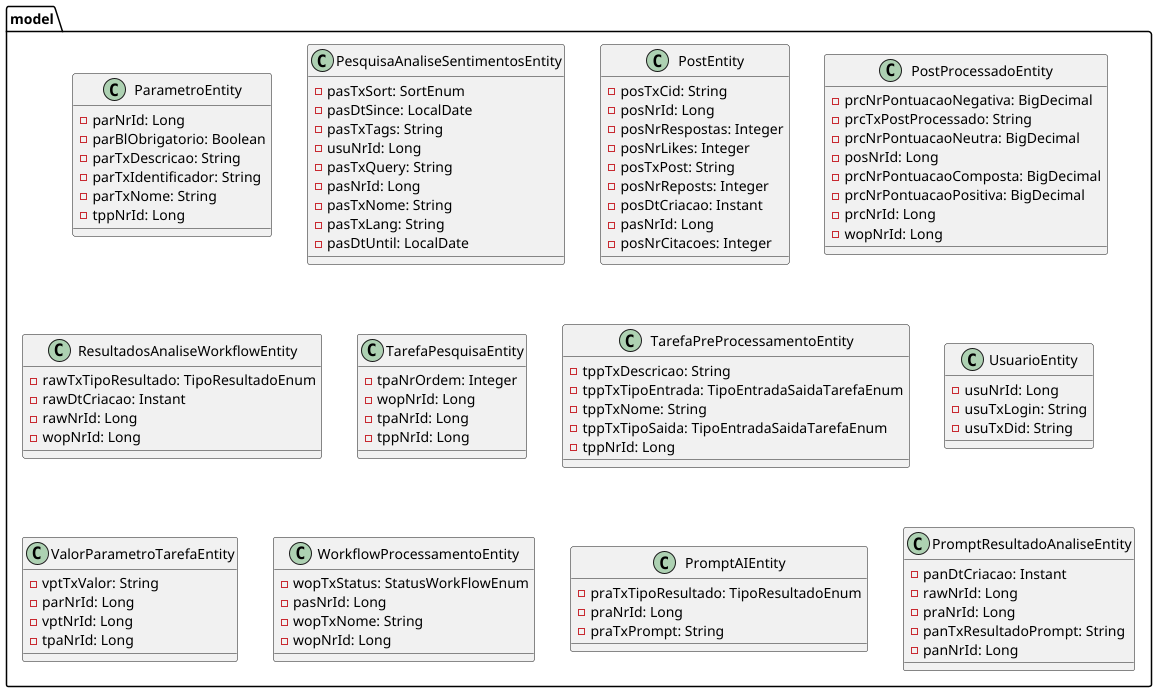
\includegraphics[scale=0.3]{imagens/sentilytics/diagramas/classes/model-classes.png}
\end{center}
}
\legend{Fonte: Autor (2025).}
\end{figure}

A \autoref{diagrama_classe_model} apresenta o Diagrama de Classes do
Pacote Model, que define as entidades utilizadas na Web API Spring Boot
do Sentilytics. Essas entidades representam as tabelas do banco de dados
e são responsáveis pelo armazenamento das informações essenciais para o
funcionamento da aplicação.

As classes do modelo seguem uma estrutura relacional, onde cada entidade
contém atributos que refletem as colunas da respectiva tabela no banco
de dados. Entre as principais entidades, destacam-se:

\begin{itemize}
\tightlist
\item
  PesquisaAnaliseSentimentosEntity: Representa uma pesquisa de análise
  de sentimentos, armazenando informações como nome, idioma, período de
  análise, critérios de busca e o usuário que criou a pesquisa;
\item
  PostEntity: Contém as postagens coletadas para análise, armazenando
  dados como conteúdo do post, quantidade de interações (curtidas,
  respostas, reposts) e data de criação;
\item
  PostProcessadoEntity: Armazena as informações das postagens após
  passarem pelo workflow de pré-processamento, incluindo o texto
  processado e as pontuações de sentimentos atribuídas;
\item
  WorkflowProcessamentoEntity: Define um workflow de processamento,
  armazenando seu nome, status e associação com uma pesquisa de análise
  de sentimentos;
\item
  TarefaPesquisaEntity e TarefaPreProcessamentoEntity: Representam as
  tarefas associadas ao workflow, incluindo ordem de execução, tipo de
  entrada/saída e descrição das operações;
\item
  ResultadosAnaliseWorkflowEntity: Armazena os resultados obtidos após a
  execução do workflow, categorizando os tipos de análise realizadas;
\item
  UsuarioEntity: Representa os usuários do sistema, armazenando
  informações como login e identificador descentralizado (DID);
\item
  ParametroEntity e ValorParametroTarefaEntity: Permitem a configuração
  dinâmica de parâmetros para personalização do workflow, garantindo
  maior flexibilidade na execução das análises;
\item
  PromptAIEntity e PromptResultadoAnaliseEntity: Armazenam os prompts e
  os resultados gerados por inteligência artificial durante a análise
  dos textos processados.
\end{itemize}

As relações entre essas entidades são fundamentais para garantir a
integridade e a consistência dos dados dentro da aplicação. Cada
entidade se relaciona diretamente com outras por meio de chaves
primárias e estrangeiras, refletindo a estrutura do banco de dados
relacional utilizado.

Para possibilitar a manipulação e persistência dessas entidades no banco
de dados, são utilizados repositórios, que fornecem uma interface para a
realização de operações como inserção, consulta, atualização e remoção
de dados. A seguir, será apresentado o Diagrama do pacote Repository,
que detalha esses componentes responsáveis pelo acesso aos dados da
aplicação.

\begin{figure}[htbp]
\hypertarget{diagram_repository}{%
\caption{Diagrama de classes da camada Repository}\label{diagram_repository}
\begin{center}
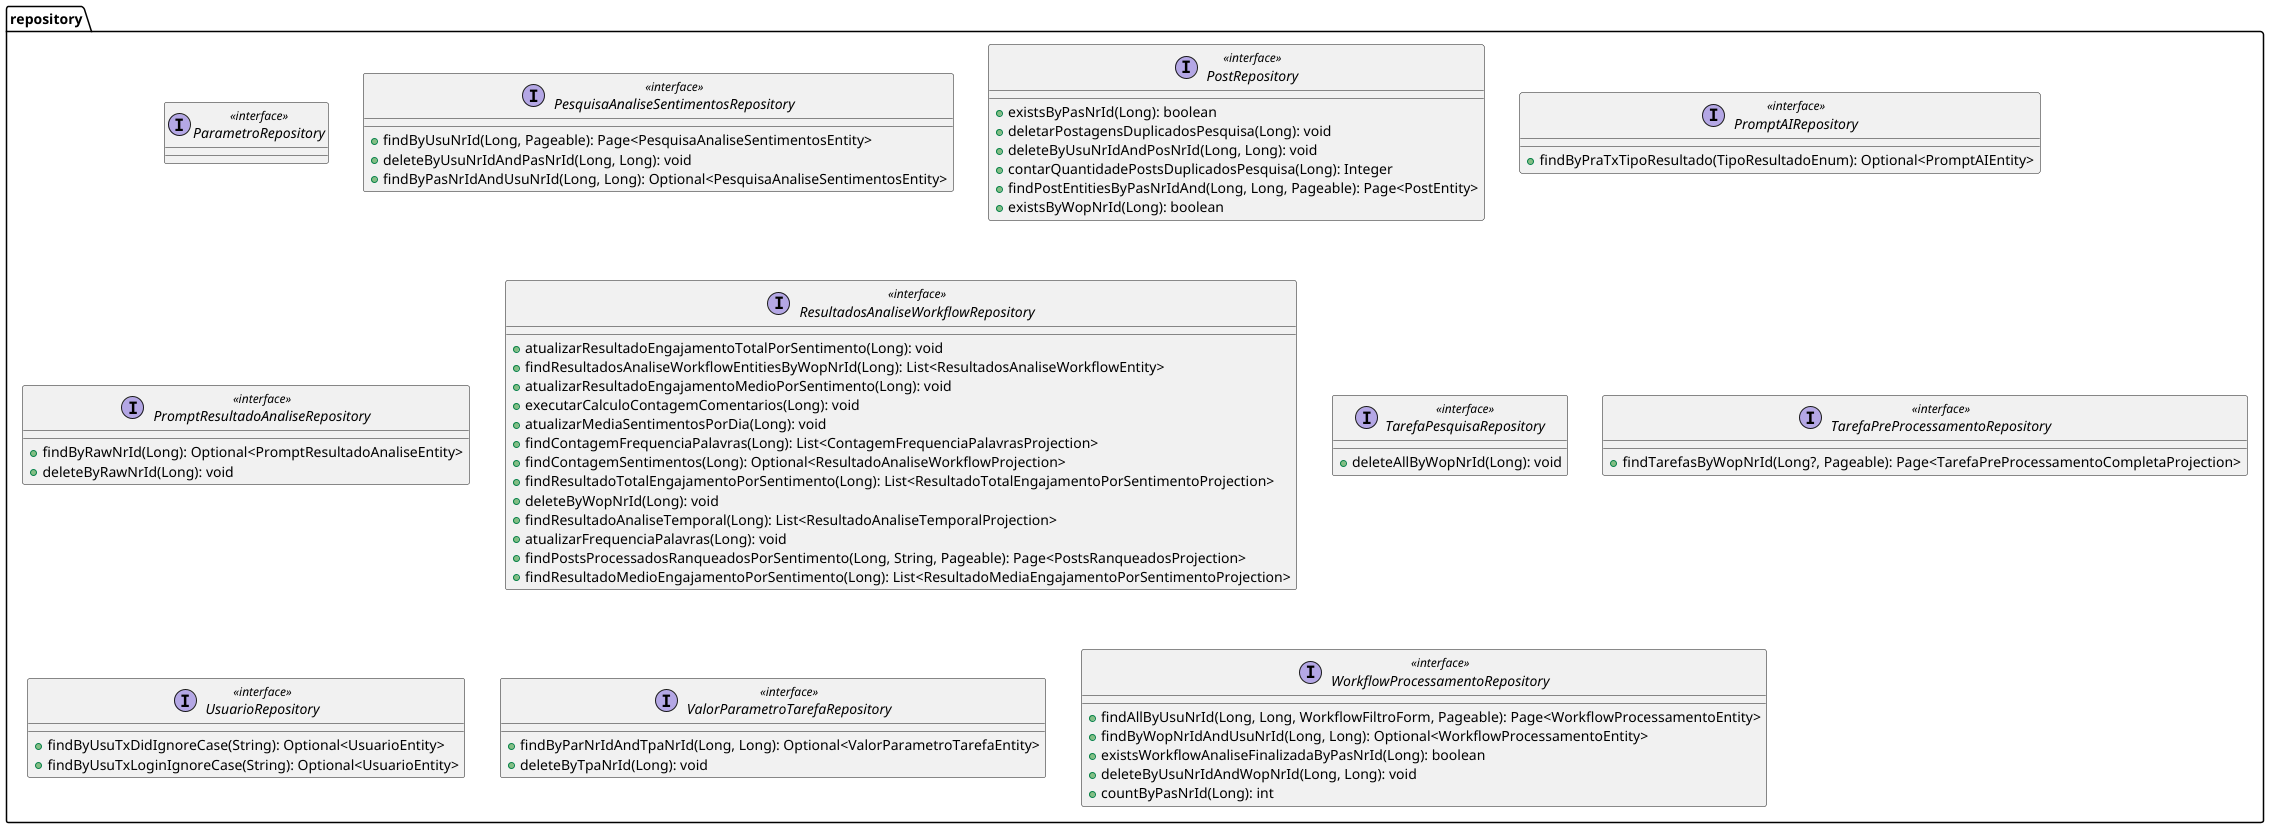
\includegraphics[scale=0.2]{imagens/sentilytics/diagramas/classes/repository-classes.png}
\end{center}
}
\legend{Fonte: Autor (2025).}
\end{figure}

A \autoref{diagram_repository} apresenta o Diagrama da Camada
Repository, responsável pelo acesso e manipulação dos dados no banco de
dados dentro da Web API Spring Boot do Sentilytics. Essa camada
implementa interfaces que utilizam o Spring Data JPA, facilitando a
execução de operações de persistência sem a necessidade de implementar
consultas SQL manualmente.

Cada repositório representa uma interface que permite a consulta,
inserção, atualização e remoção de registros no banco de dados,
fornecendo métodos específicos para manipulação das entidades da
aplicação. Entre os principais repositórios, destacam-se:

\begin{itemize}
\tightlist
\item
  PesquisaAnaliseSentimentosRepository: Gerencia as pesquisas de análise
  de sentimentos, possibilitando operações como busca por usuário,
  exclusão de pesquisas e recuperação de registros específicos;
\item
  PostRepository: Manipula os dados das postagens coletadas, permitindo
  verificar duplicações, realizar exclusões e consultar postagens
  associadas a uma pesquisa;
\item
  WorkflowProcessamentoRepository: Responsável pelo armazenamento e
  recuperação dos workflows de processamento, permitindo buscar
  registros vinculados a um usuário ou pesquisa, além de verificar a
  existência de análises finalizadas;
\item
  ResultadosAnaliseWorkflowRepository: Garante a persistência dos
  resultados gerados pelo workflow, oferecendo métodos para calcular
  métricas, como engajamento médio e frequência de palavras, além de
  realizar consultas sobre o desempenho da análise de sentimentos ao
  longo do tempo;
\item
  PromptAIRepository e PromptResultadoAnaliseRepository: Permitem a
  recuperação e exclusão de prompts de IA e seus respectivos resultados
  de análise, utilizados na interpretação automática dos textos
  processados;
\item
  TarefaPesquisaRepository e TarefaPreProcessamentoRepository: Fornecem
  métodos para gerenciamento das tarefas do workflow, permitindo a
  exclusão de tarefas e a listagem das configurações associadas ao
  processo de pré-processamento;
\item
  UsuarioRepository: Responsável pela recuperação das informações de
  usuários, permitindo buscas por identificador descentralizado (DID) ou
  login;
\item
  ValorParametroTarefaRepository: Manipula os parâmetros personalizados
  das tarefas do workflow, possibilitando consultas e exclusões de
  valores associados às configurações definidas pelo usuário.
\end{itemize}

Para processar os dados e aplicar as regras de negócio da aplicação, os
repositórios são utilizados pela camada Service, que implementa a lógica
necessária para a manipulação dessas informações. A seguir, será
apresentado o Diagrama da Camada Service, detalhando os serviços
responsáveis pelo processamento e gestão das regras de negócio do
Sentilytics.

\begin{figure}[htbp]
\hypertarget{diagram_service}{%
\caption{Diagrama de classes do pacote Services}\label{diagram_service}
\begin{center}
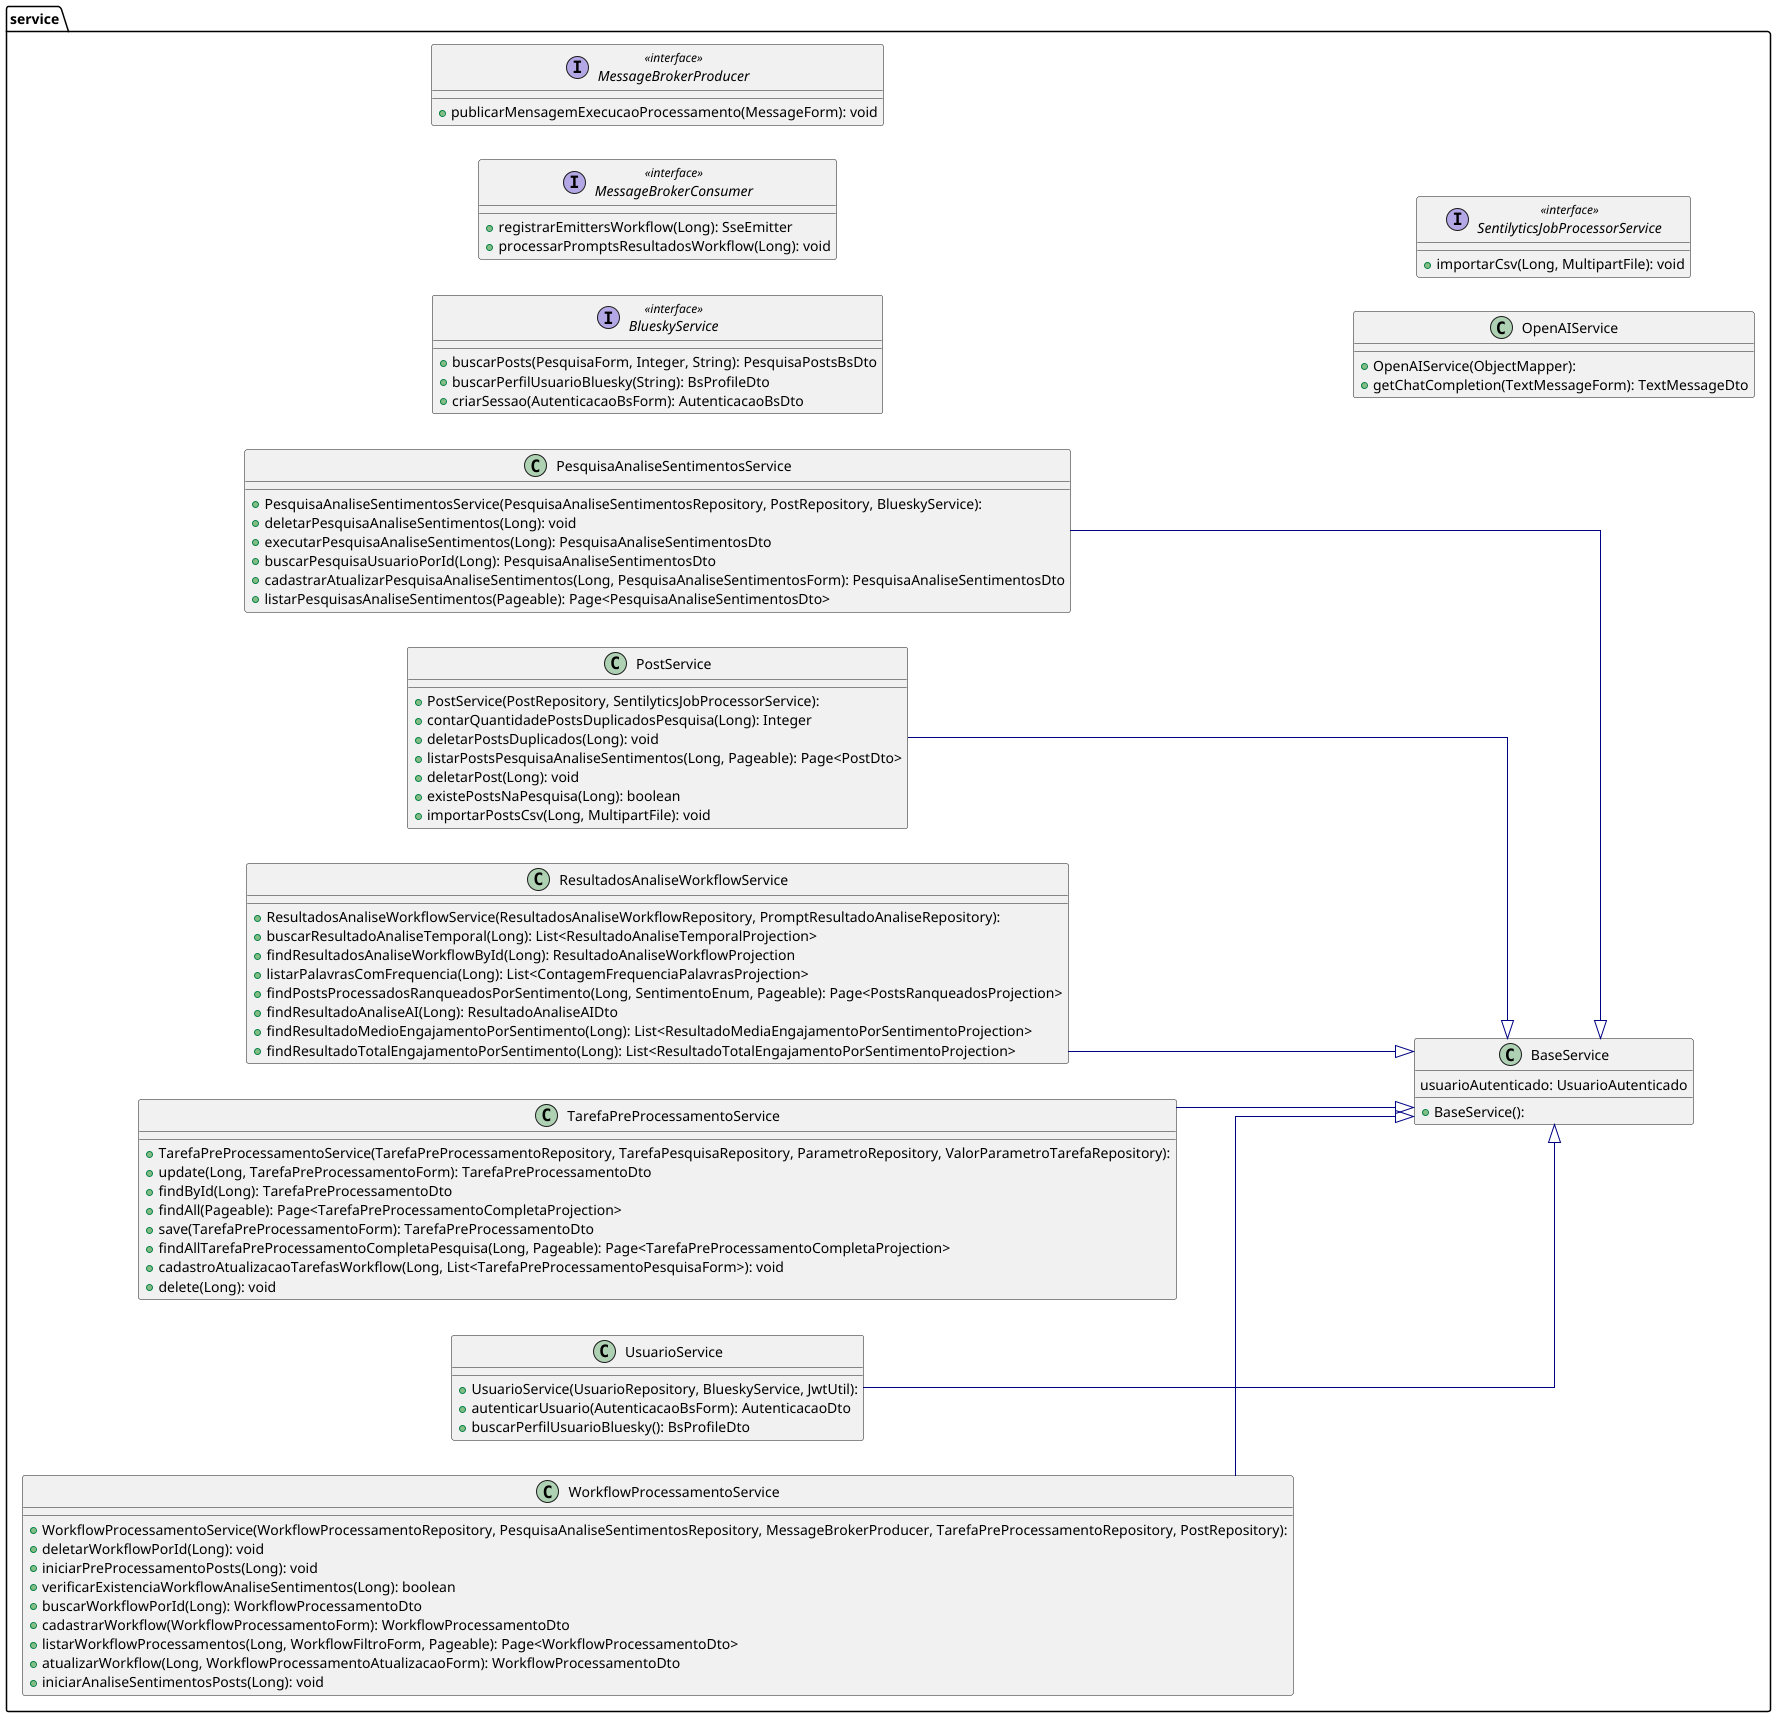
\includegraphics[scale=0.2]{imagens/sentilytics/diagramas/classes/service-classes.png}
\end{center}
}
\legend{Fonte: Autor (2025).}
\end{figure}

A \autoref{diagram_service} apresenta o Diagrama da Camada Service,
responsável por implementar a lógica de negócio da Web API Spring Boot
do Sentilytics. Essa camada é responsável pelo processamento das
operações da aplicação, garantindo a manipulação dos dados, a aplicação
das regras de negócio e a interação entre os controladores e os
repositórios.

As classes de serviço estendem a classe BaseService, que fornece
funcionalidades comuns para gerenciamento de usuários autenticados e
outras operações compartilhadas. A seguir, destacam-se algumas das
principais responsabilidades dessa camada:

\begin{itemize}
\tightlist
\item
  PesquisaAnaliseSentimentosService: Gerencia as operações relacionadas
  às pesquisas de análise de sentimentos, permitindo cadastrar,
  atualizar, listar e excluir pesquisas, além de executar buscas de
  postagens vinculadas;
\item
  PostService: Responsável pela manipulação das postagens coletadas,
  oferecendo funcionalidades para listagem, exclusão de duplicatas e
  importação de posts via CSV;
\item
  WorkflowProcessamentoService: Controla os workflows de processamento,
  permitindo cadastrar, atualizar e excluir workflows, além de iniciar
  as etapas de pré-processamento e análise de sentimentos;
\item
  ResultadosAnaliseWorkflowService: Gerencia a recuperação dos
  resultados das análises, fornecendo consultas sobre frequência de
  palavras, engajamento e posts processados;
\item
  TarefaPreProcessamentoService: Implementa as regras para gerenciamento
  das tarefas dentro dos workflows, permitindo o cadastro, atualização e
  exclusão de funções que compõem o pré-processamento de textos;
\item
  UsuarioService: Gerencia a autenticação de usuários e a integração com
  Bluesky, permitindo que os usuários recuperem perfis e autentiquem
  suas sessões;
\item
  Interfaces de Comunicação: Além dos serviços internos, a camada inclui
  interfaces, como BlueskyService (para comunicação com a API externa do
  Bluesky), MessageBrokerProducer (para publicar mensagens no RabbitMQ)
  e MessageBrokerConsumer (para processar eventos de mensagens
  recebidas).
\end{itemize}

A camada de serviços é essencial para garantir que a lógica da aplicação
esteja desacoplada da camada de persistência e dos controladores,
promovendo organização, reusabilidade e escalabilidade.

Para expor essas funcionalidades aos usuários e ao \emph{front-end} da
aplicação, a camada Service se conecta diretamente com a Camada
Controller, que será abordada a seguir. O próximo diagrama apresentará
os controladores da API, responsáveis por receber requisições, validar
os dados de entrada e encaminhar as chamadas aos serviços apropriados.

\begin{figure}[htbp]
\hypertarget{diagram_controller}{%
\caption{Diagrama de classes do pacote controllers}\label{diagram_controller}
\begin{center}
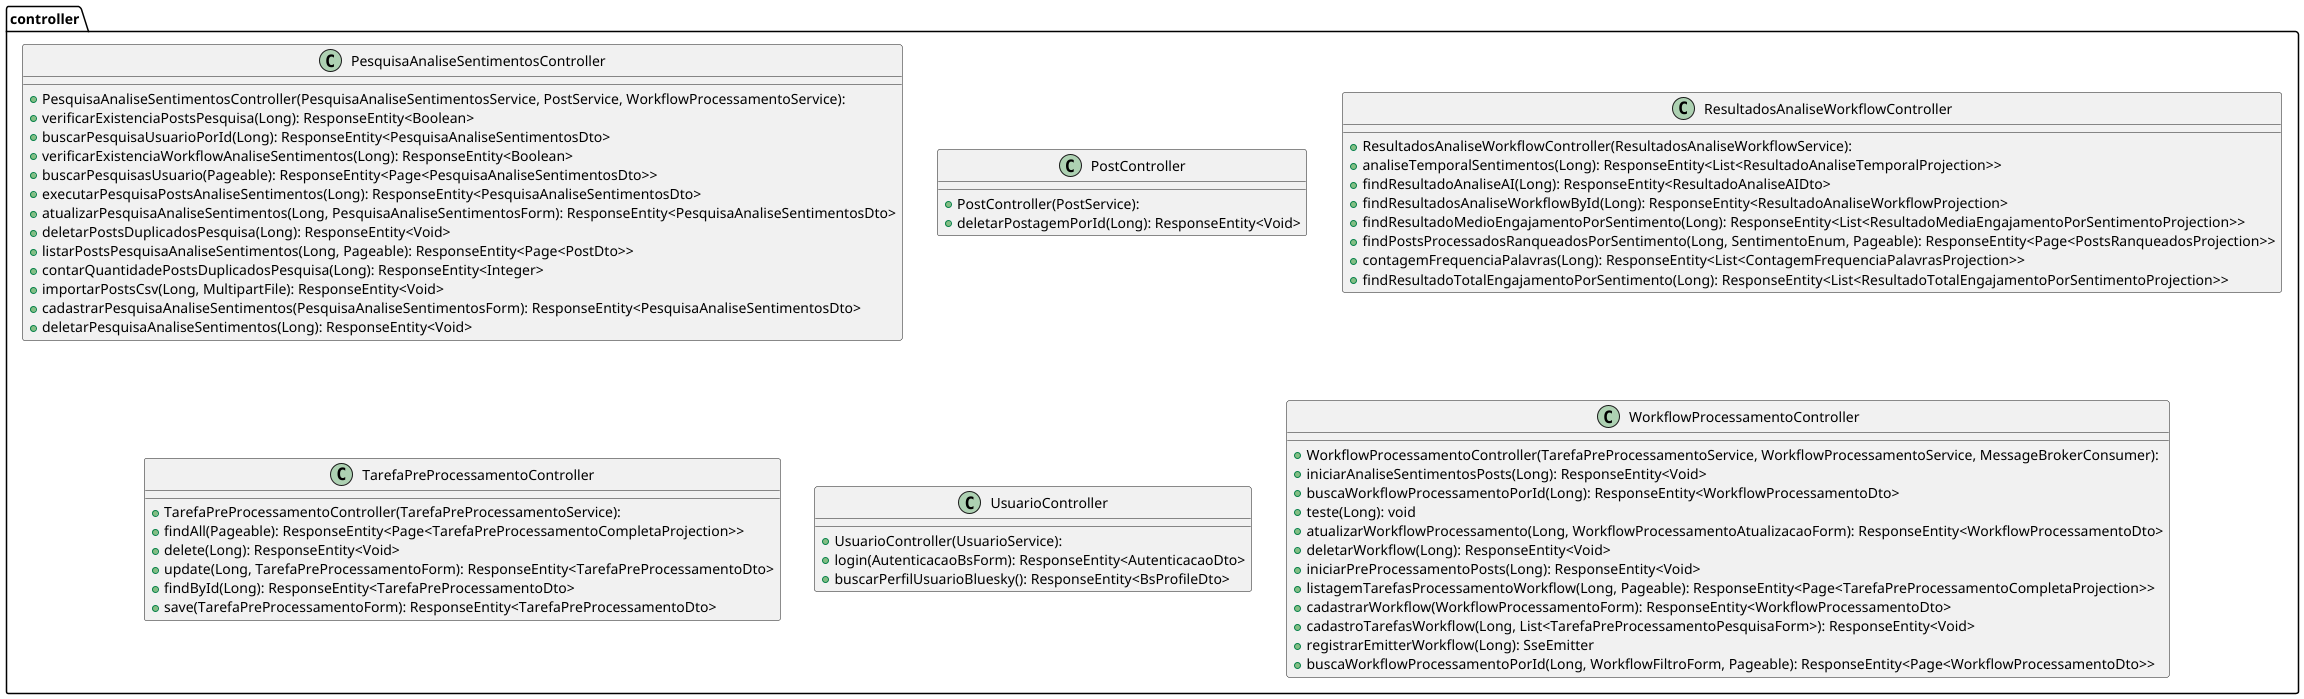
\includegraphics[scale=0.2]{imagens/sentilytics/diagramas/classes/controller-classes.png}
\end{center}
}
\legend{Fonte: Autor (2025).}
\end{figure}

A \autoref{diagram_controller} apresenta o Diagrama da Camada
Controller, responsável por gerenciar as requisições HTTP e expor os
endpoints da API. Essa camada atua como intermediária entre o
\emph{front-end} e a lógica de negócio, direcionando as requisições
recebidas para os serviços apropriados e retornando as respostas
processadas ao cliente.

Os controladores seguem a estrutura RESTful, organizando os endpoints de
acordo com as funcionalidades da aplicação. A seguir, destacam-se os
principais componentes dessa camada:

\begin{itemize}
\tightlist
\item
  PesquisaAnaliseSentimentosController: Gerencia operações relacionadas
  às pesquisas de análise de sentimentos, permitindo ao usuário criar,
  atualizar, listar e excluir pesquisas, além de buscar postagens
  associadas e importar dados via CSV;
\item
  PostController: Responsável por excluir postagens específicas,
  garantindo a manutenção dos dados armazenados na plataforma;
\item
  WorkflowProcessamentoController: Controla a execução dos workflows de
  processamento, possibilitando cadastro, atualização e remoção de
  workflows, além de iniciar as etapas de pré-processamento e análise de
  sentimentos. Esse controlador também fornece endpoints para consulta e
  manipulação das tarefas dentro de um workflow;
\item
  ResultadosAnaliseWorkflowController: Disponibiliza os resultados
  gerados pela análise de sentimentos, incluindo frequência de palavras,
  análise temporal, engajamento médio e posts processados por
  sentimento;
\item
  TarefaPreProcessamentoController: Permite a gestão das tarefas de
  pré-processamento, fornecendo operações para cadastro, atualização,
  listagem e remoção de tarefas associadas ao processamento textual;
\item
  UsuarioController: Gerencia a autenticação de usuários e a integração
  com a plataforma Bluesky, possibilitando o login e a recuperação de
  perfis. Os controladores utilizam ResponseEntity para padronizar as
  respostas da API, garantindo que cada requisição retorne um código de
  status adequado, além dos dados processados.
\end{itemize}

\hypertarget{diagrama-de-componentes}{%
\subsection{Diagrama de Componentes}\label{diagrama-de-componentes}}

O Diagrama de Componentes é uma representação da estrutura da aplicação,
destacando os principais serviços que a compõem e suas interações. Ele
permite visualizar a separação dos módulos, auxiliando na manutenção e
na compreensão da arquitetura do sistema.

No Sentilytics, a solução é composta por diferentes serviços que atuam
de forma conjunta para viabilizar o fluxo de análise de sentimentos. A
\autoref{diagrama_componentes} apresenta essa composição:

A \autoref{diagrama_componentes} a seguir apresenta a organização e a
comunicação entre esses componentes.

\begin{figure}[htbp]
\hypertarget{diagrama_componentes}{%
\caption{Diagrama de Componentes da Solução}\label{diagrama_componentes}
\begin{center}
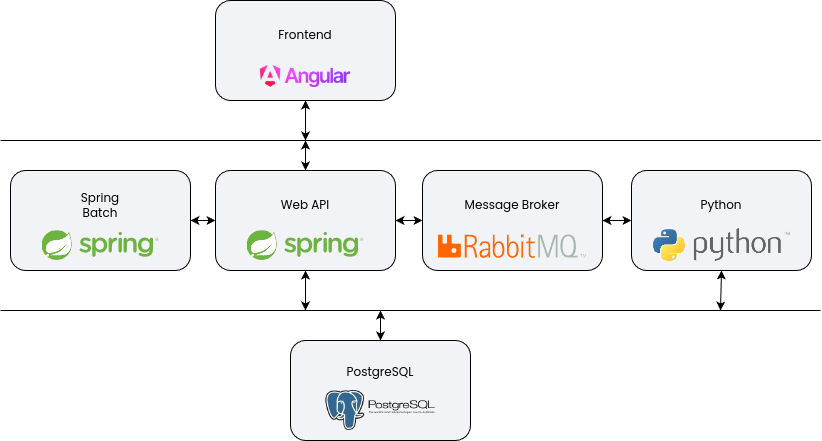
\includegraphics[scale=0.4]{imagens/sentilytics/diagramas/diagrama_componentes.png}
\end{center}
}
\legend{Fonte: Autor (2025).}
\end{figure}

Cada um dos componentes desempenha um papel essencial dentro da
arquitetura do Sentilytics. A seguir, são apresentados detalhes sobre o
funcionamento e a responsabilidade de cada módulo:

\begin{itemize}
\tightlist
\item
  Aplicação Python -- Responsável pelo pré-processamento e análise de
  sentimentos das postagens, recebe as mensagens da fila do Message
  Broker para processar e envia mensagens para a fila quando um processo
  finaliza;
\item
  RabbitMQ -- Atua como broker de mensagens, permitindo comunicação
  assíncrona entre a aplicação Python e a Web API Spring Boot;
\item
  Aplicação Spring Batch -- Processa o arquivo CSV que contem as
  postagens em lote e faz a carga das postagens importadas no banco de
  dados;
\item
  Web API Spring Boot -- Exposição dos serviços da aplicação via API
  REST para o Angular, interligando todos os módulos;
\item
  Front-end Angular -- Interface do usuário para interação com a
  plataforma;
\item
  Banco de Dados PostgreSQL -- Armazena pesquisas, postagens e
  resultados da análise de sentimentos.
\end{itemize}

\hypertarget{interfaces-gruxe1fica}{%
\subsection{Interfaces gráfica}\label{interfaces-gruxe1fica}}

A interface gráfica é um dos principais pontos de interação entre os
usuários e a aplicação, sendo responsável por garantir uma experiência
intuitiva na utilização do Sentilytics. Para o desenvolvimento da
interface, foi utilizado o \emph{framework} Angular.

A interface foi projetada para oferecer um fluxo de navegação claro e
acessível, permitindo que os usuários cadastrem e configurem pesquisas,
acompanhem o processamento dos dados e analisem os resultados da análise
de sentimentos.

Nesta seção, são apresentadas as telas e componentes principais da
interface do Sentilytics, detalhando a funcionalidade de cada interface
e a forma como os usuários interagem com o sistema.

O primeiro ponto de contato do usuário com a aplicação ocorre na tela de
login, que possibilita a autenticação no sistema. A seguir, é
apresentada essa interface, destacando seus principais componentes e
funcionalidades.

\begin{figure}[htbp]
\hypertarget{tela_login}{%
\caption{Tela de Login do Sentilytics}\label{tela_login}
\begin{center}
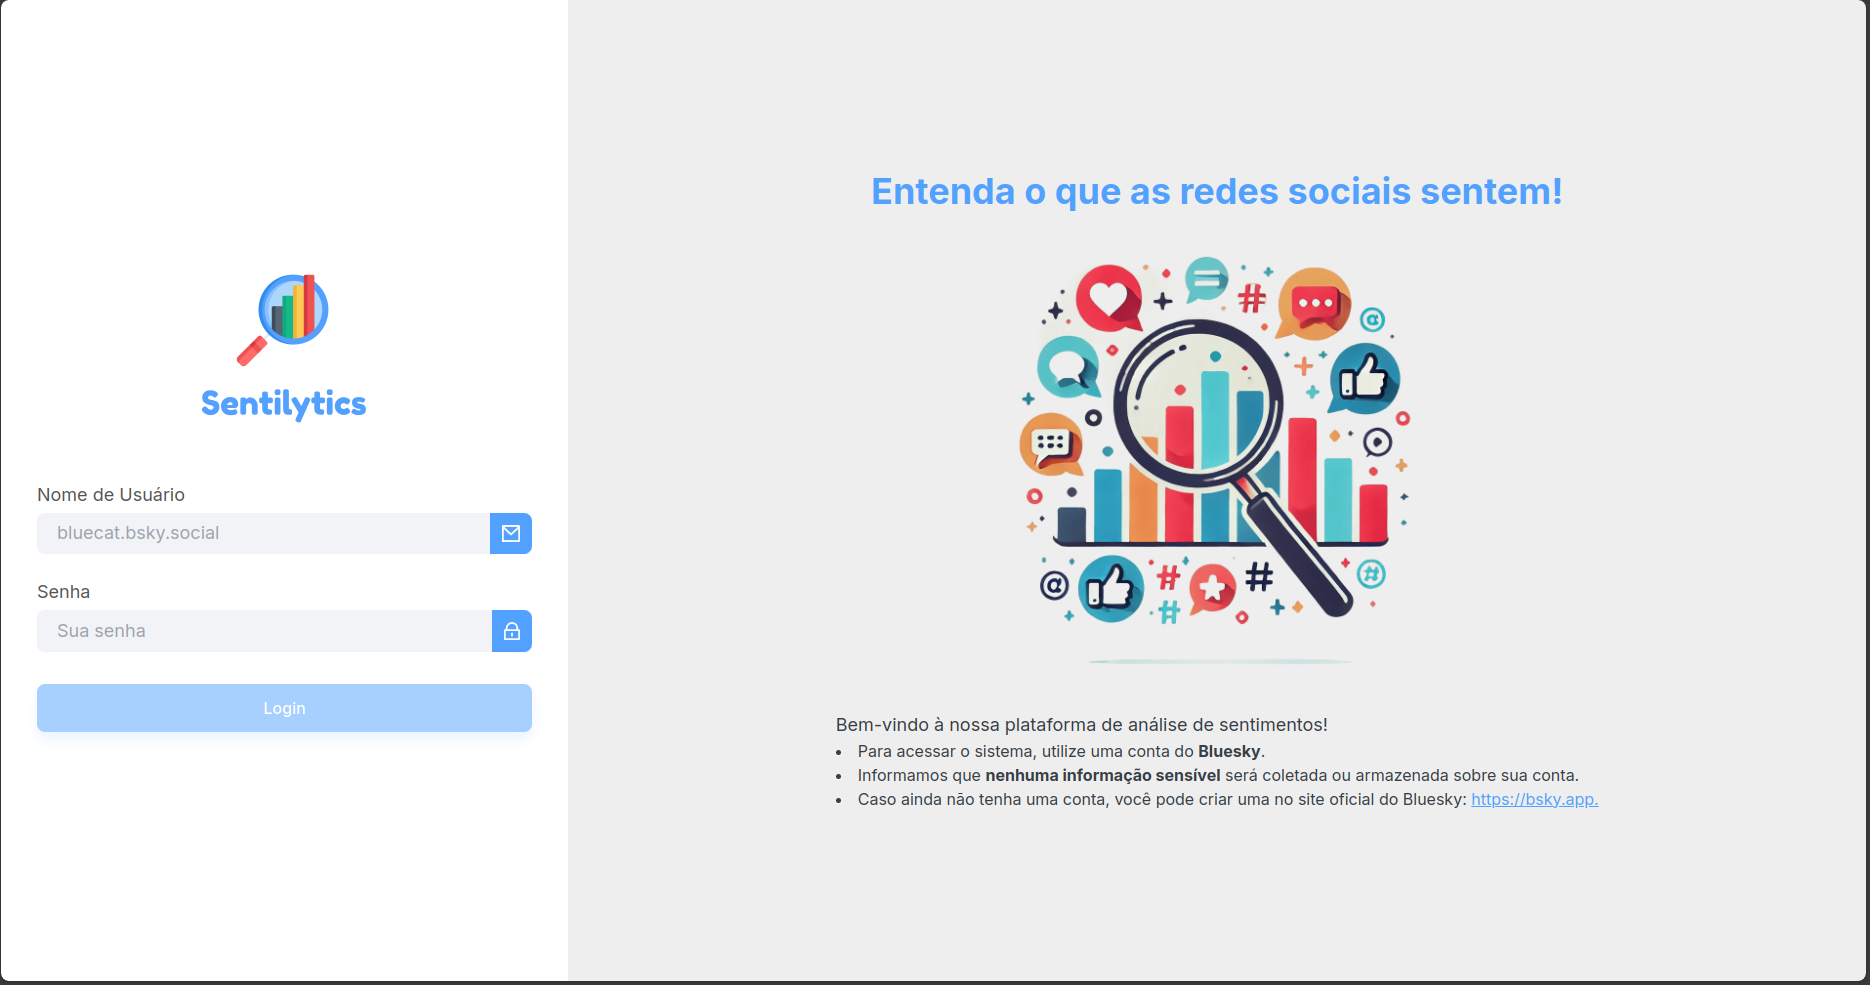
\includegraphics[scale=0.2]{imagens/sentilytics/interface-grafica/tela-login.png}
\end{center}
}
\legend{Fonte: Autor (2025).}
\end{figure}

A tela de login é a porta de entrada para o acesso ao Sentilytics,
permitindo apenas a autenticação. Para manter a segurança e a
simplicidade no gerenciamento de contas, o sistema utiliza o serviço do
Bluesky como principal método de autenticação. Dessa forma, toda a
criação ou administração de contas ocorre diretamente no Bluesky.

Ao inserir as credenciais corretas, o sistema valida as informações
diretamente com a API do Bluesky, garantindo a autenticação segura. Caso
as credenciais sejam inválidas, o usuário recebe um aviso para revisar
os dados informados.

Essa abordagem proporciona uma experiência simplificada para o usuário,
eliminando a necessidade de criar e lembrar novas senhas, ao mesmo tempo
em que mantém um padrão seguro e confiável de autenticação. Após a
autenticação, o usuário é direcionado para a tela de listagem de
pesquisas, onde pode visualizar todas as análises de sentimentos já
criadas.

\begin{figure}[htbp]
\hypertarget{tela_listagem_pesquisas}{%
\caption{Tela de Listagem de Pesquisas}\label{tela_listagem_pesquisas}
\begin{center}
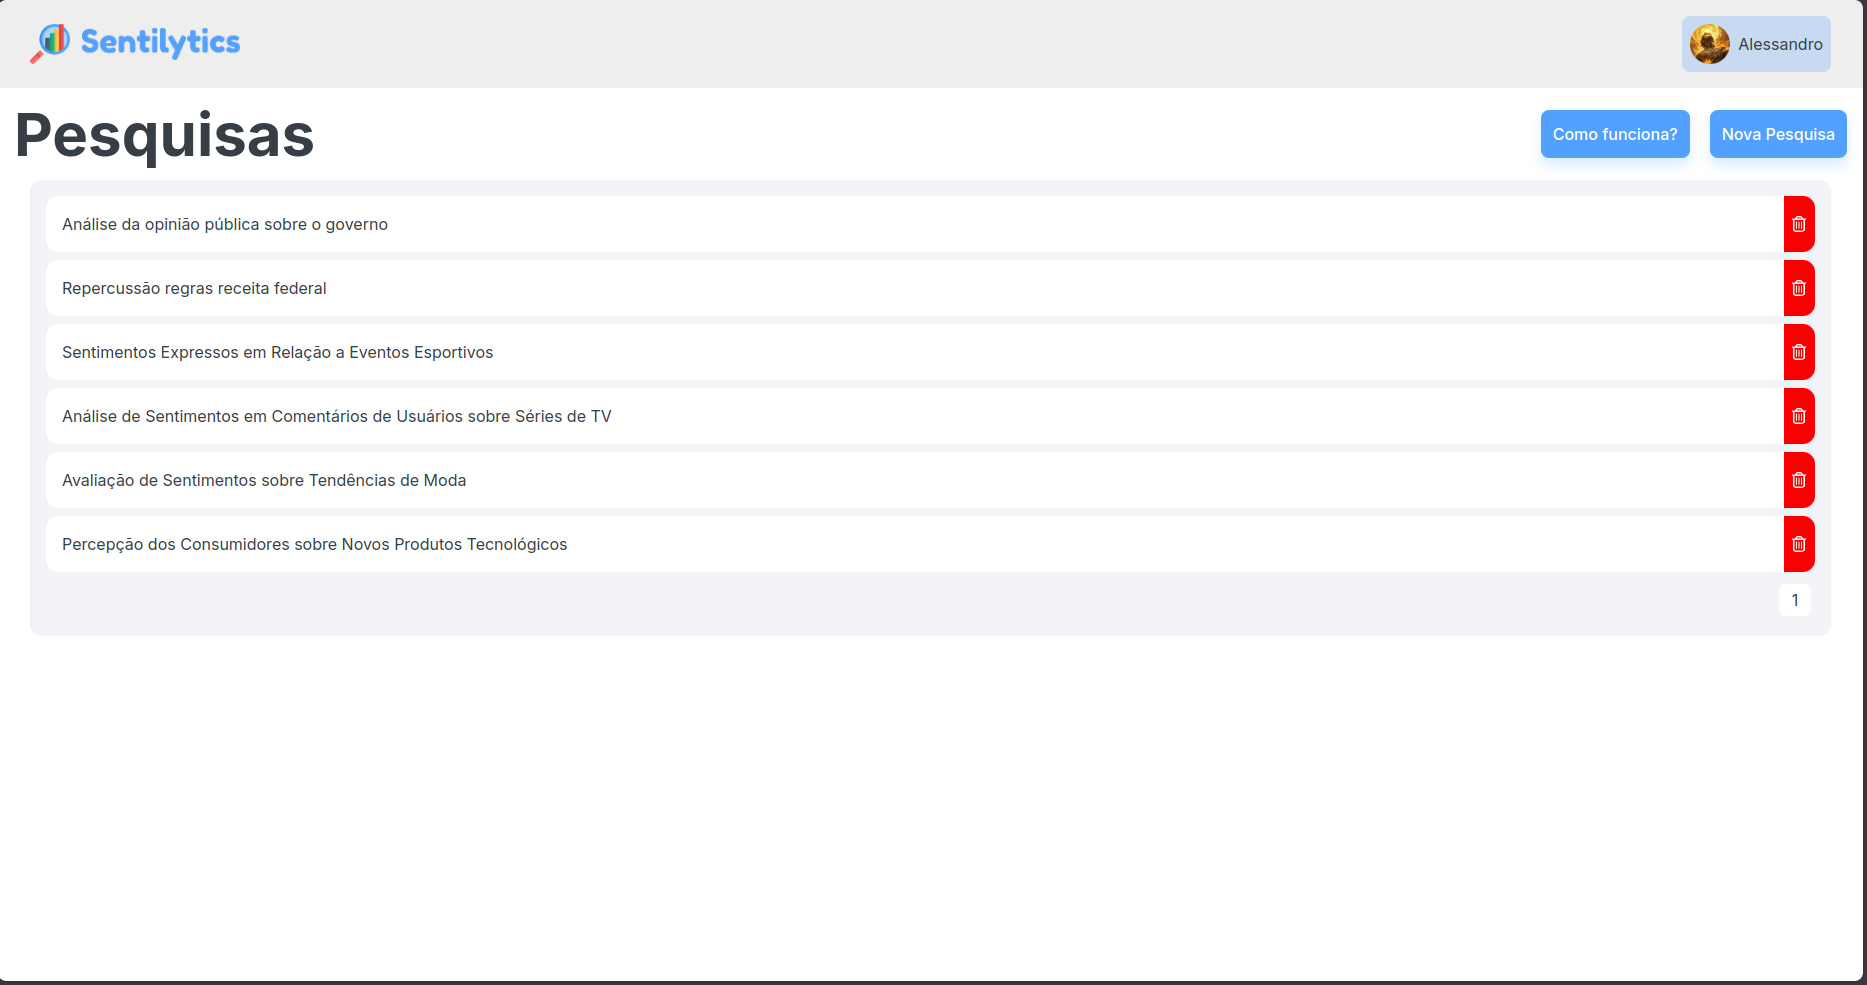
\includegraphics[scale=0.2]{imagens/sentilytics/interface-grafica/listagem-pesquisas.png}
\end{center}
}
\legend{Fonte: Autor (2025).}
\end{figure}

Após a autenticação, o usuário é direcionado para a tela de listagem de
pesquisas, onde pode visualizar todas as pesquisas de análise de
sentimentos já criadas.

Nesta tela, o usuário tem a opção de cadastrar ou deletar uma pesquisa,
onde ao clicar no botão ``Cadastrar Pesquisa'', uma janela modal é
exibida solicitando o nome da pesquisa e a query inicial de busca. Após
a confirmação do cadastro, a nova pesquisa é adicionada à lista.

Para acessar os detalhes de uma pesquisa já cadastrada, o usuário pode
selecioná-la na listagem, sendo automaticamente redirecionado para a
tela de visualização da pesquisa, onde poderá acompanhar e gerenciar os
dados coletados.

\begin{figure}[htbp]
\hypertarget{tela_dados_pesquisa}{%
\caption{Tela de Exibição da Pesquisa}\label{tela_dados_pesquisa}
\begin{center}
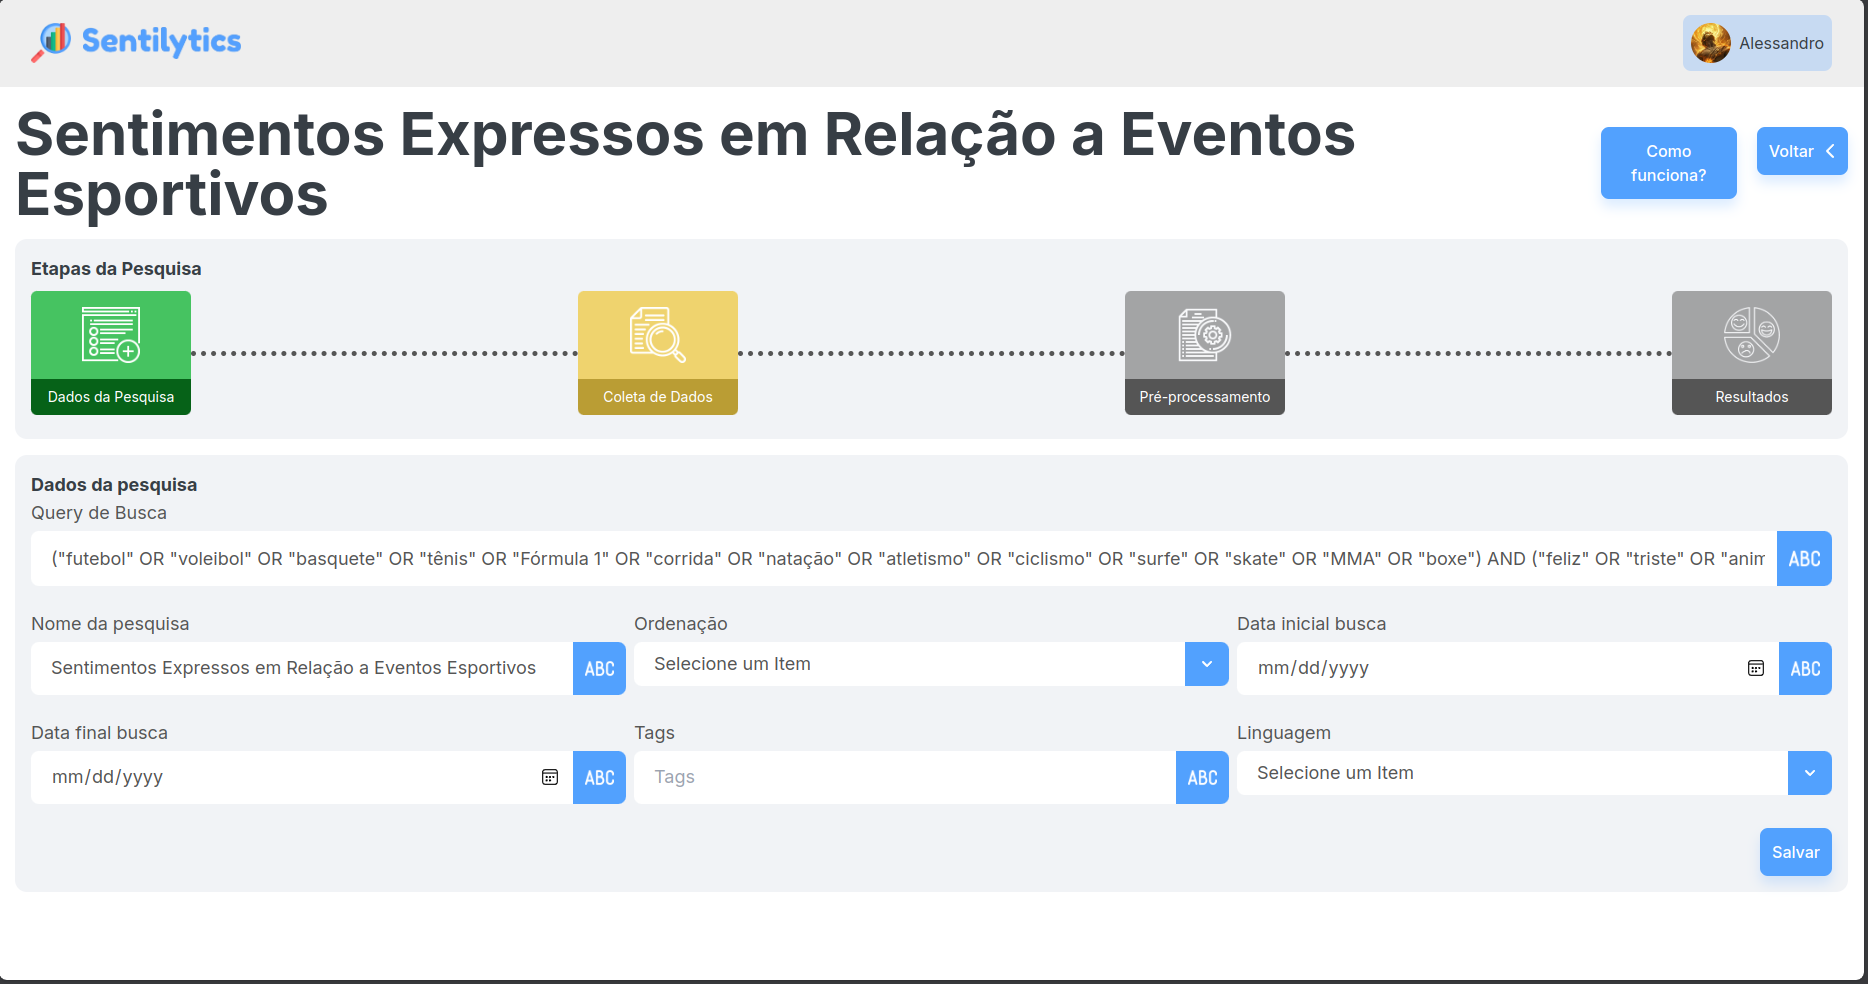
\includegraphics[scale=0.2]{imagens/sentilytics/interface-grafica/dados-pesquisa.png}
\end{center}
}
\legend{Fonte: Autor (2025).}
\end{figure}

A tela da pesquisa mostrada na \autoref{tela_dados_pesquisa} é a
interface central para o gerenciamento de uma análise de sentimentos
dentro do Sentilytics. Essa tela organiza o fluxo do usuário em quatro
etapas, representadas por botões dispostos em sequência:

\begin{enumerate}
\def\labelenumi{\arabic{enumi})}
\tightlist
\item
  Dados da Pesquisa;
\item
  Coleta de Dados;
\item
  Pré-processamento;
\item
  Resultados.
\end{enumerate}

Cada etapa pode ser clicada para alternar os elementos exibidos abaixo,
permitindo que o usuário navegue entre as diferentes fases do processo
de análise. Para facilitar a visualização do progresso, as etapas são
coloridas conforme seu estado atual:

\begin{itemize}
\tightlist
\item
  Verde -- Etapa concluída, indicando que todas as ações necessárias
  foram realizadas;
\item
  Amarelo -- Etapa pendente, sinalizando que há ações a serem executadas
  antes de avançar;
\item
  Cinza -- Etapa inacessível, indicando que ainda há pré-requisitos a
  serem cumpridos antes de prosseguir.
\end{itemize}

No primeiro acesso, o usuário visualiza a aba ``Dados da Pesquisa'',
onde pode configurar ou alterar as informações utilizadas na busca de
postagens, caso a coleta de dados via Bluesky seja ativada.

Cada uma das próximas etapas é liberada de acordo com a sequência do
fluxo, garantindo que o usuário siga um processo estruturado para a
realização da pesquisa.

A etapa atual exibida na \autoref{tela_dados_pesquisa} é a ``Dados da
Pesquisa'', nesse momento o usuário pode visualizar e modificar as
informações da pesquisa. Esses dados serão utilizados caso o usuário
opte por realizar a coleta automática de postagens através da rede
social Bluesky. Essa configuração permite definir os critérios de busca
que serão aplicados na obtenção dos posts, garantindo que a análise de
sentimentos seja realizada com base em conteúdos relevantes.

\begin{figure}[htbp]
\hypertarget{tela_coleta_dados_pesquisa}{%
\caption{Etapa de Coleta de Dados}\label{tela_coleta_dados_pesquisa}
\begin{center}
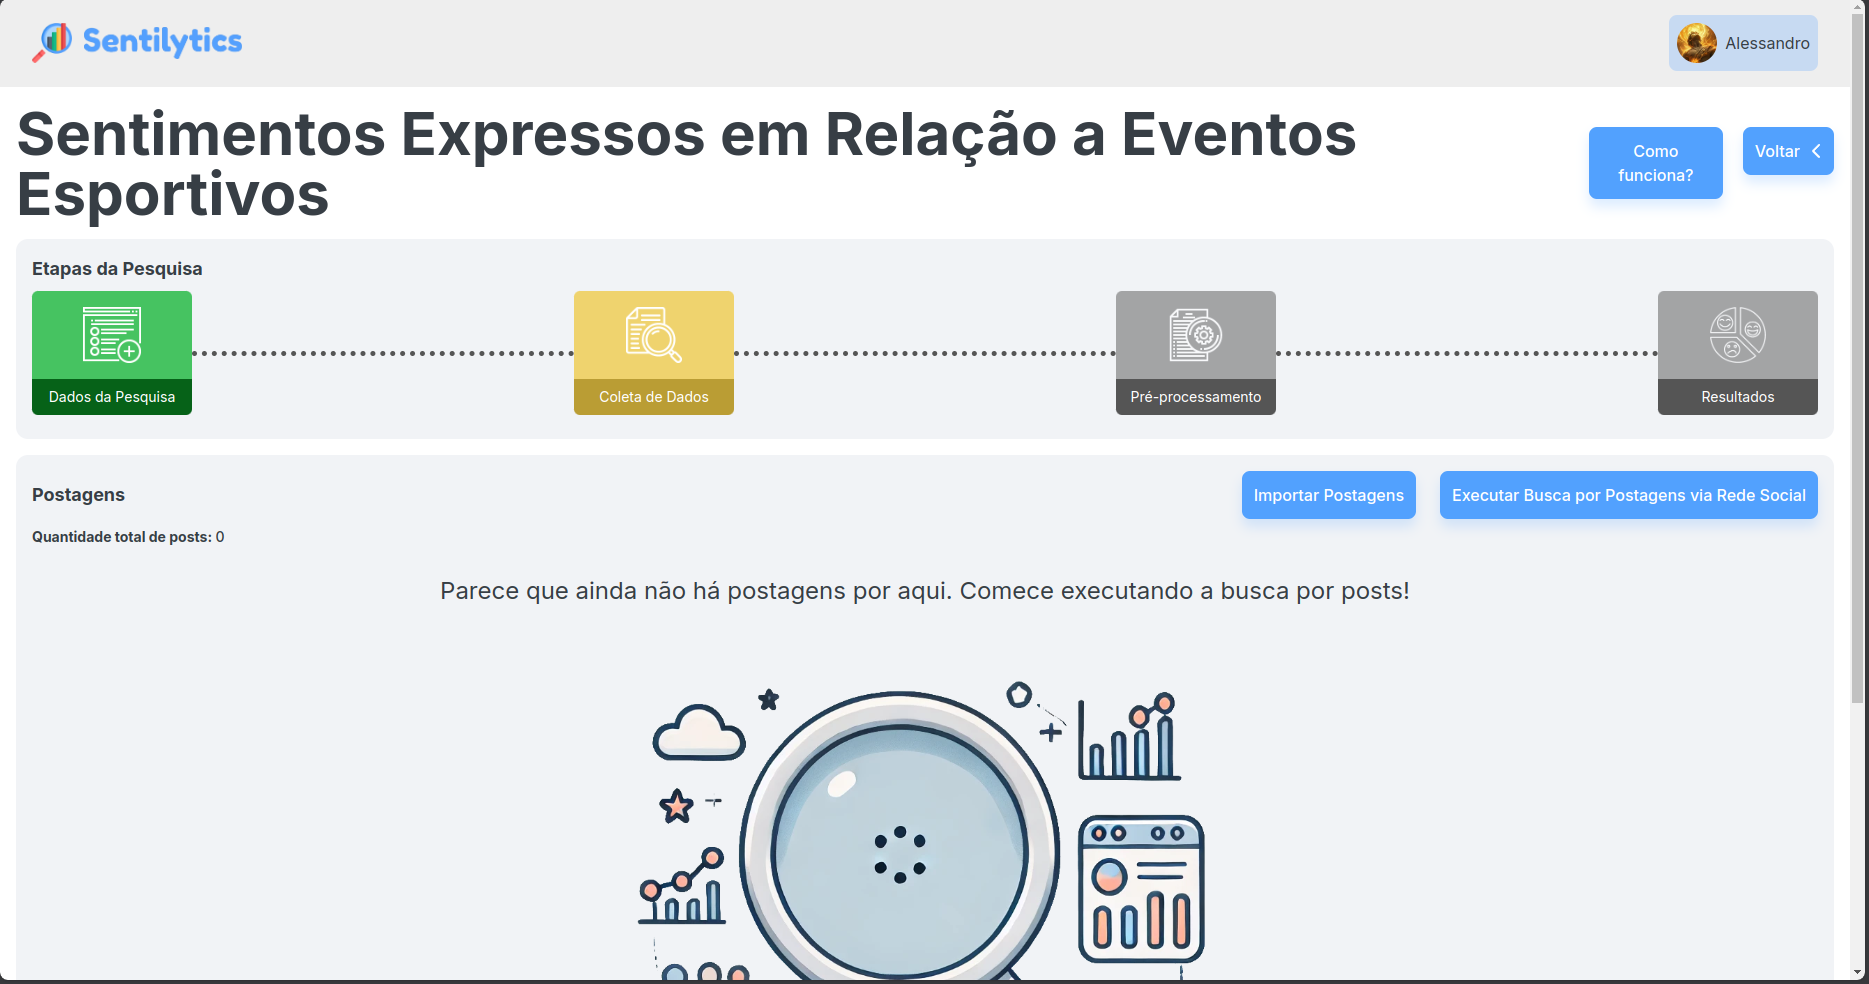
\includegraphics[scale=0.2]{imagens/sentilytics/interface-grafica/coleta-dados.png}
\end{center}
}
\legend{Fonte: Autor (2025).}
\end{figure}

Após definir os dados da pesquisa, o próximo passo é a coleta de
postagens, onde o usuário pode importar dados manualmente ou realizar a
busca automática via Bluesky. Na \autoref{tela_coleta_dados_pesquisa} é
mostrada a etapa de coleta dos dados, nessa fase o usuário pode
gerenciar as postagens que serão analisadas no Sentilytics. O usuário
pode visualizar os posts já armazenados no sistema e optar por adicionar
novos dados por meio de duas opções de coleta:

\begin{itemize}
\tightlist
\item
  Busca automática no Bluesky -- O sistema realiza uma pesquisa na rede
  social Bluesky, coletando postagens conforme os critérios definidos na
  etapa anterior;
\item
  Importação via CSV -- O usuário pode carregar um arquivo contendo
  postagens previamente coletadas. Para auxiliar nesse processo, a
  interface exibe um tutorial explicativo, orientando como preparar o
  arquivo corretamente.
\end{itemize}

Além da adição de novos posts, a tela também oferece a opção de excluir
postagens específicas, permitindo ao usuário refinar os dados que serão
utilizados na análise.

Com os posts devidamente coletados e organizados, o usuário pode avançar
para a próxima etapa: o processamento, onde os textos serão preparados
para a análise de sentimentos.

\begin{figure}[htbp]
\hypertarget{tela_processamento}{%
\caption{Etapa de Processamento}\label{tela_processamento}
\begin{center}
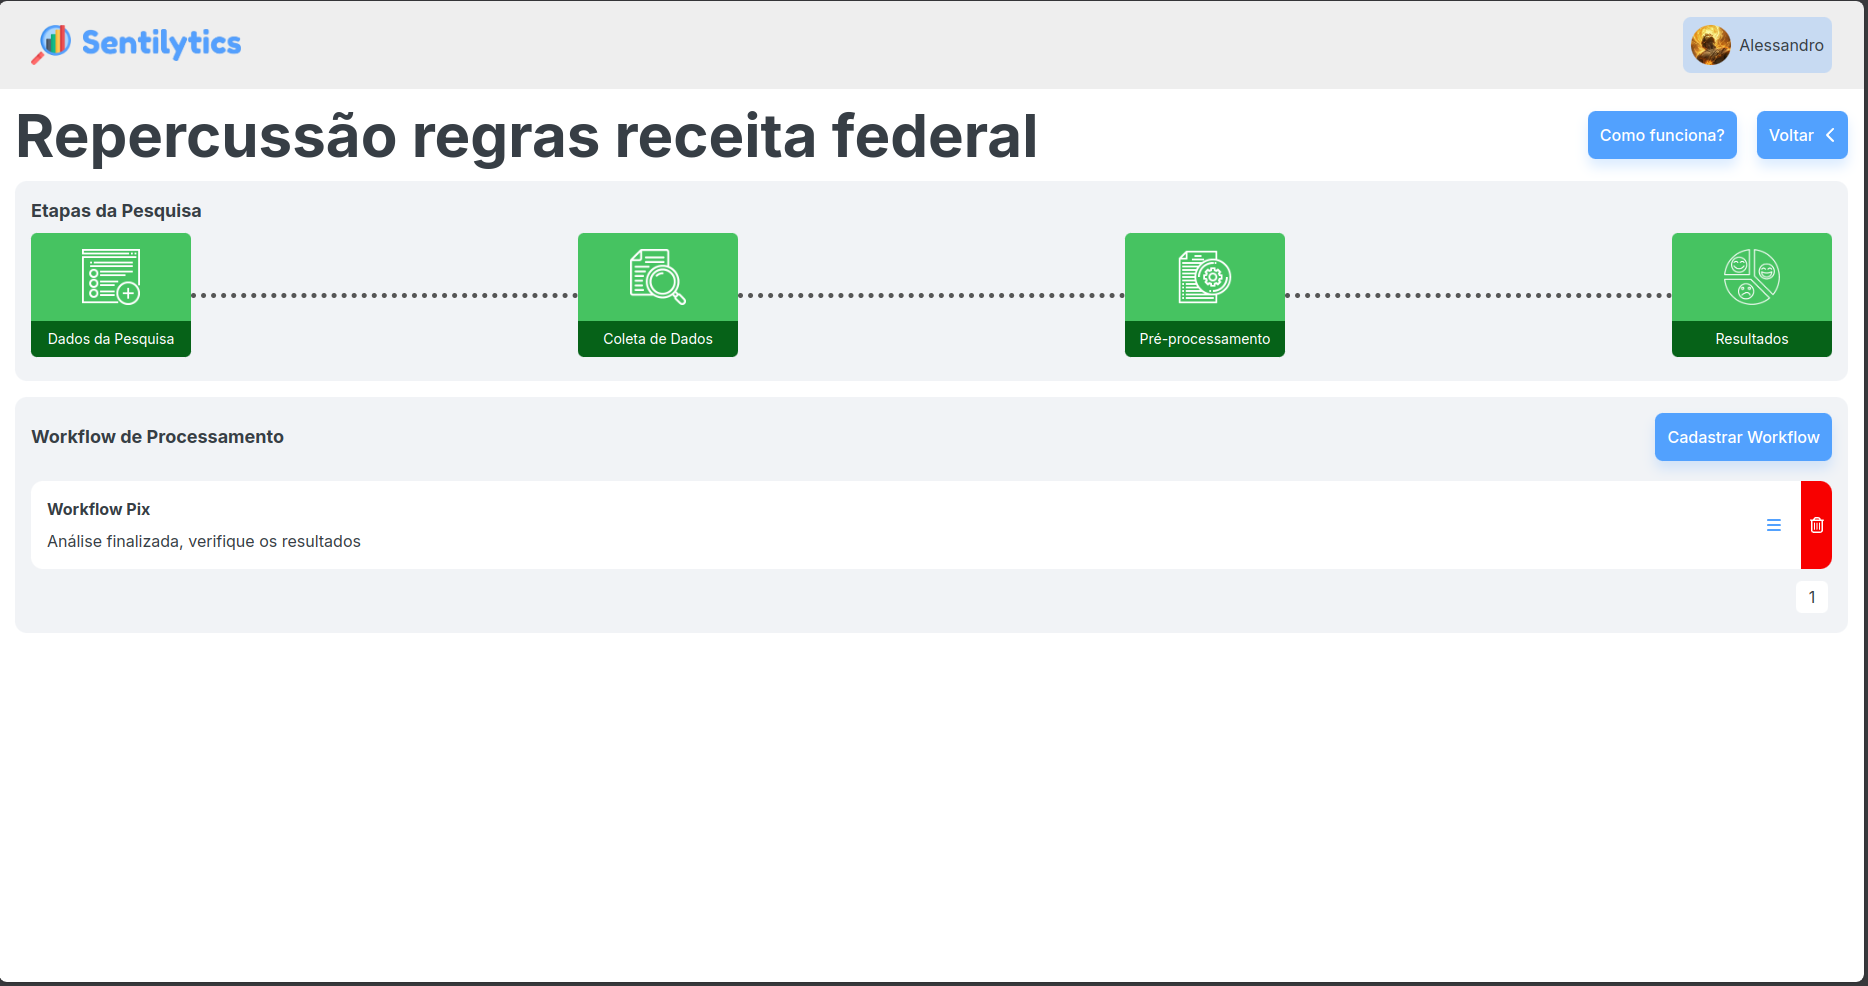
\includegraphics[scale=0.2]{imagens/sentilytics/interface-grafica/processamento.png}
\end{center}
}
\legend{Fonte: Autor (2025).}
\end{figure}

A \autoref{tela_processamento} mostra a etapa de processamento, onde o
usuário pode configurar e executar as etapas necessárias para preparar e
analisar as postagens coletadas. Nessa passo, o usuário pode criar um
workflow, que define a sequência de tarefas de pré-processamento
aplicadas aos textos antes da análise de sentimentos.

As principais ações disponíveis nesta etapa incluem:

\begin{itemize}
\tightlist
\item
  Criar um workflow -- O usuário pode definir um novo fluxo de
  pré-processamento, adicionando as tarefas que serão aplicadas às
  postagens antes da análise de sentimentos;
\item
  Excluir um workflow -- Caso um workflow não seja mais necessário, ele
  pode ser removido do sistema;
\item
  Executar o pré-processamento -- Após a criação do workflow, o usuário
  pode iniciar o pré-processamento, que realiza transformações nos
  textos coletados, como normalização e remoção de elementos
  indesejados;
\item
  Executar a análise de sentimentos -- Quando o pré-processamento é
  concluído, o usuário pode prosseguir com a análise de sentimentos,
  onde as postagens processadas são classificadas de acordo com suas
  emoções ou polaridade textual.
\end{itemize}

O pré-processamento e a análise de sentimentos podem ser repetidos
quantas vezes forem necessárias dentro de um workflow, permitindo
ajustes na configuração e refinamento dos resultados.

É importante pontuar que caso novas postagens sejam adicionadas após um
workflow já ter sido executado, elas não serão automaticamente
refletidas nos resultados anteriores. Para incluir as novas postagens na
análise, o workflow precisa ser processado novamente, garantindo que
todas as postagens passem pelas etapas de pré-processamento e análise de
sentimentos.

Com o workflow finalizado, o usuário pode avançar para a última etapa do
processo: a visualização dos resultados, onde os \emph{insights}
extraídos das postagens processadas são apresentados de forma
estruturada.

\begin{figure}[htbp]
\hypertarget{etapa_resultados}{%
\caption{Etapa de Resultados}\label{etapa_resultados}
\begin{center}
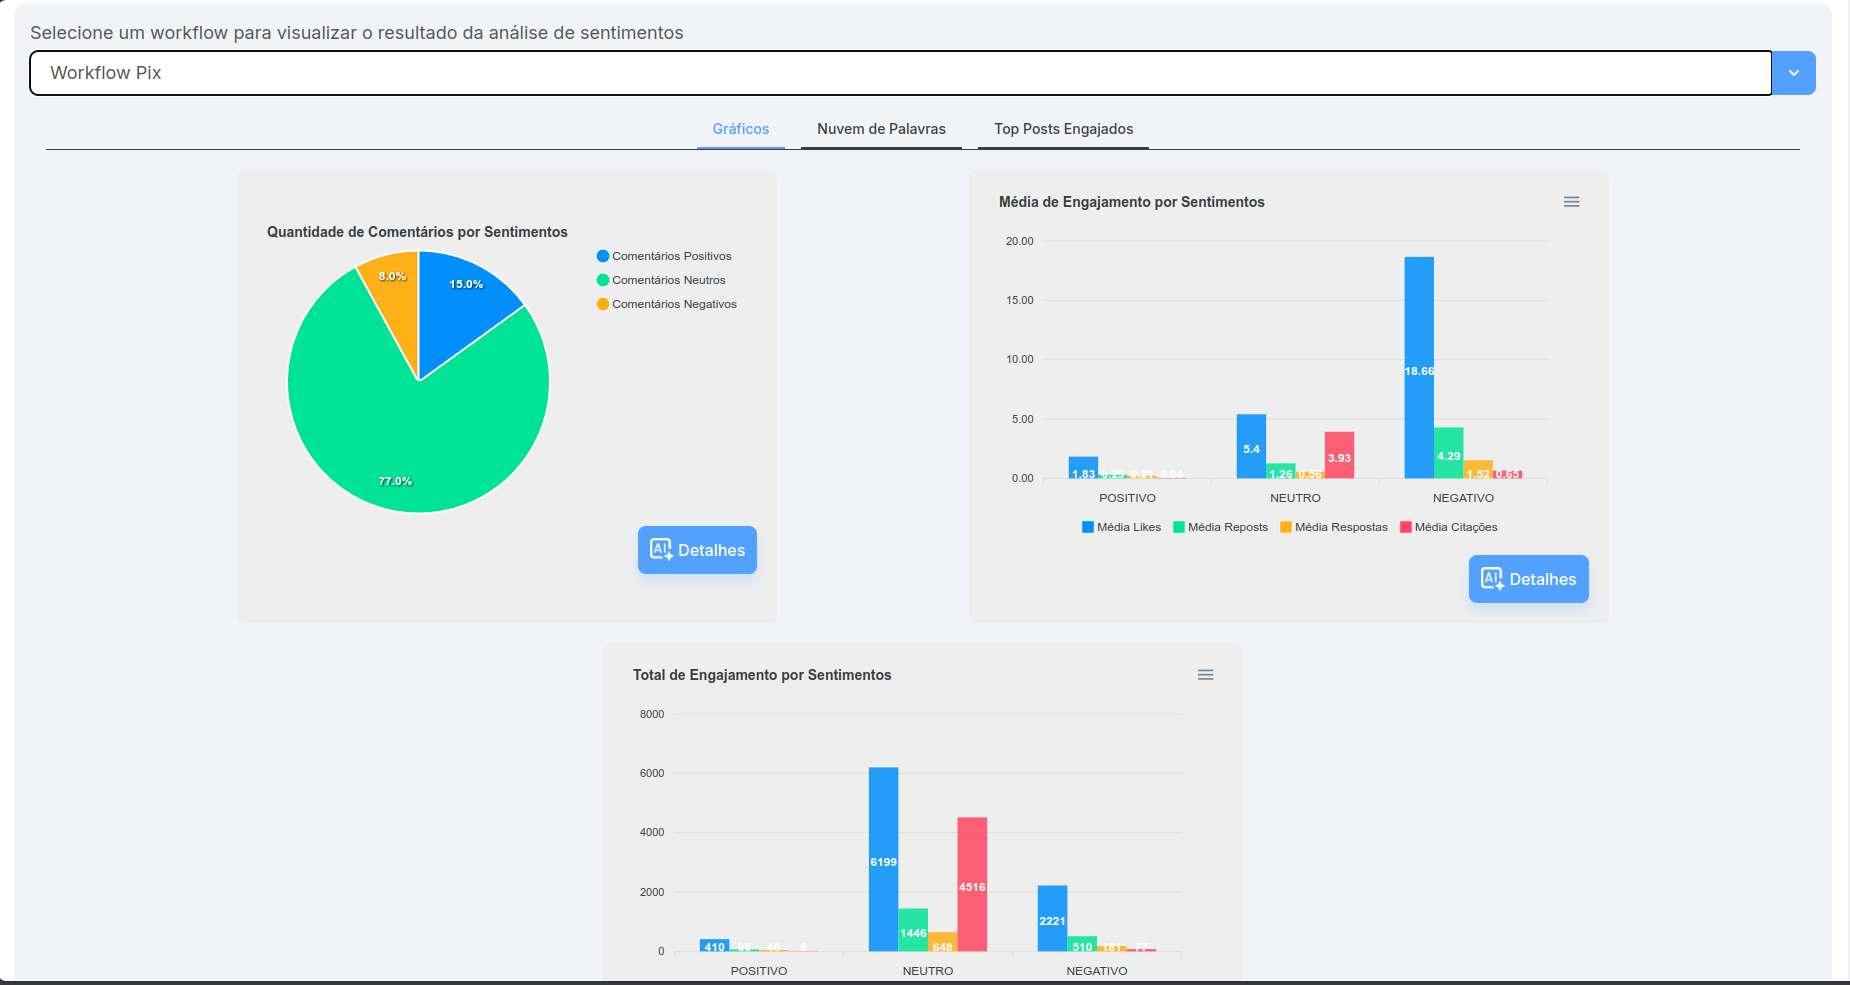
\includegraphics[scale=0.2]{imagens/sentilytics/interface-grafica/resultado-graficos.png}
\end{center}
}
\legend{Fonte: Autor (2025).}
\end{figure}

A etapa de resultados mostrado na \autoref{etapa_resultados} permite ao
usuário visualizar e interpretar os dados processados a partir da
análise de sentimentos. Para acessar essa etapa, é necessário selecionar
um workflow que já tenha passado pelo processo completo de
pré-processamento e análise de sentimentos. Após a seleção do workflow,
o restante do conteúdo da tela é exibido, oferecendo três abas
principais para exploração dos resultados:

\begin{enumerate}
\def\labelenumi{\arabic{enumi})}
\tightlist
\item
  Aba de Gráficos Essa aba apresenta quatro gráficos interativos, que
  auxiliam na compreensão da distribuição dos sentimentos e do impacto
  das postagens analisadas:
\end{enumerate}

\begin{itemize}
\tightlist
\item
  Quantidade de Comentários por Sentimentos -- Um gráfico de pizza que
  exibe a porcentagem e o número total de postagens classificadas em
  cada sentimento;
\item
  Média de Engajamento por Sentimentos -- Um gráfico de barras verticais
  que relaciona a média de curtidas, reposts, respostas e citações para
  cada tipo de sentimento identificado;
\item
  Total de Engajamento por Sentimentos -- Um gráfico de barras verticais
  que exibe o total acumulado de interações (likes, reposts, respostas e
  citações) para cada sentimento;
\item
  Análise Temporal de Sentimentos -- Um gráfico que acompanha a variação
  dos sentimentos ao longo do tempo, permitindo identificar tendências e
  padrões emocionais nos dados coletados.
\end{itemize}

\begin{enumerate}
\def\labelenumi{\arabic{enumi})}
\item
  Aba de Nuvem de Palavras - Nesta aba, é exibida uma nuvem de palavras
  gerada a partir dos textos processados. Essa visualização destaca as
  palavras mais frequentes nas postagens analisadas, permitindo uma
  análise rápida dos termos mais relevantes dentro do contexto dos
  dados;
\item
  Aba de Top Posts Engajados - Essa aba apresenta uma listagem dos posts
  mais engajados, ranqueados com base no número de curtidas, respostas,
  reposts e citações. Além disso, há um filtro por sentimento,
  permitindo que o usuário explore os posts de acordo com suas
  classificações emocionais.
\end{enumerate}

Cada post exibido nesta listagem pode ser visualizado em sua forma
original e após o pré-processamento, permitindo que o usuário compreenda
como as transformações realizadas impactaram o conteúdo analisado.

\begin{figure}[htbp]
\hypertarget{qrcode}{%
\caption{QRCode com link para o vídeo}\label{qrcode}
\begin{center}

\includegraphics[scale=0.6]{imagens/sentilytics/qr_code.png}
\end{center}
}
\legend{Fonte: Autor (2025).}
\end{figure}

Para complementar o entendimento do processo descrito, a
\autoref{qrcode} apresenta um QR Code que direciona para um vídeo
demonstrativo. No vídeo, é possível acompanhar de forma prática e
detalhada todas as etapas da criação de uma pesquisa de análise de
sentimentos no Sentilytics, desde a autenticação até a visualização dos
resultados.

\hypertarget{escala-de-trabalho-6x1-um-estudo-de-caso-com-o-sentilytics}{%
\chapter{Escala de trabalho 6x1: um estudo de caso com o
Sentilytics}\label{escala-de-trabalho-6x1-um-estudo-de-caso-com-o-sentilytics}}

A jornada de trabalho é um dos principais temas debatidos no contexto
organizacional, influenciando diretamente a qualidade de vida dos
trabalhadores e a produtividade das empresas. Entre os modelos de
escalas mais utilizados, a escala 6x1 (seis dias de trabalho seguidos
por um dia de descanso) é amplamente adotada em diversos setores, como
comércio, indústria e serviços.

A rotina dessa escala gera debates sobre sua eficácia e os impactos na
saúde física e mental dos trabalhadores, além da influência na
satisfação e no desempenho profissional. Com a crescente digitalização
das relações trabalhistas e a disseminação de opiniões nas redes
sociais, é possível analisar como os trabalhadores percebem essa jornada
de trabalho por meio de ferramentas de análise de sentimentos.

O presente estudo tem como objetivo aplicar a ferramenta Sentilytics
para realizar uma análise de sentimentos sobre a escala 6x1, utilizando
dados extraídos da rede social Bluesky. O foco será examinar a
polaridade dos sentimentos (positivo, negativo ou neutro) relacionados
às experiências e percepções da população sobre esse regime de trabalho.

\hypertarget{muxe9todologia-do-estudo}{%
\section{Métodologia do estudo}\label{muxe9todologia-do-estudo}}

Este estudo de caso possui uma abordagem exploratória com elementos
descritivos. A abordagem exploratória se justifica pelo fato de que o
Sentilytics ainda não foi amplamente utilizado para análise de
sentimentos relacionados a modelos de jornada de trabalho, tornando
necessário um levantamento inicial sobre seu comportamento, desafios e
limitações.

Dessa forma, o estudo busca compreender como a ferramenta processa
postagens coletadas no Bluesky sobre a escala 6x1, identificando padrões
e dificuldades na análise dos sentimentos expressos pelos trabalhadores.
Além disso, a pesquisa possui um caráter descritivo, pois detalha as
etapas da coleta, pré-processamento e análise dos dados, além de
apresentar os resultados encontrados, permitindo uma visão estruturada
sobre as percepções dos usuários a respeito da escala 6x1.

\hypertarget{coleta-de-dados}{%
\subsection{Coleta de Dados}\label{coleta-de-dados}}

A coleta de dados foi realizada por meio da integração da ferramenta
Sentilytics com o Bluesky. Com a pesquisa já criada, será necessário
configurar os parâmetros que serão utilizados para a busca, podemos
visualizar essa tela na \autoref{configuracao_pesquisa}.

\begin{figure}[htbp]
\hypertarget{configuracao_pesquisa}{%
\caption{Configuração da pesquisa}\label{configuracao_pesquisa}
\begin{center}
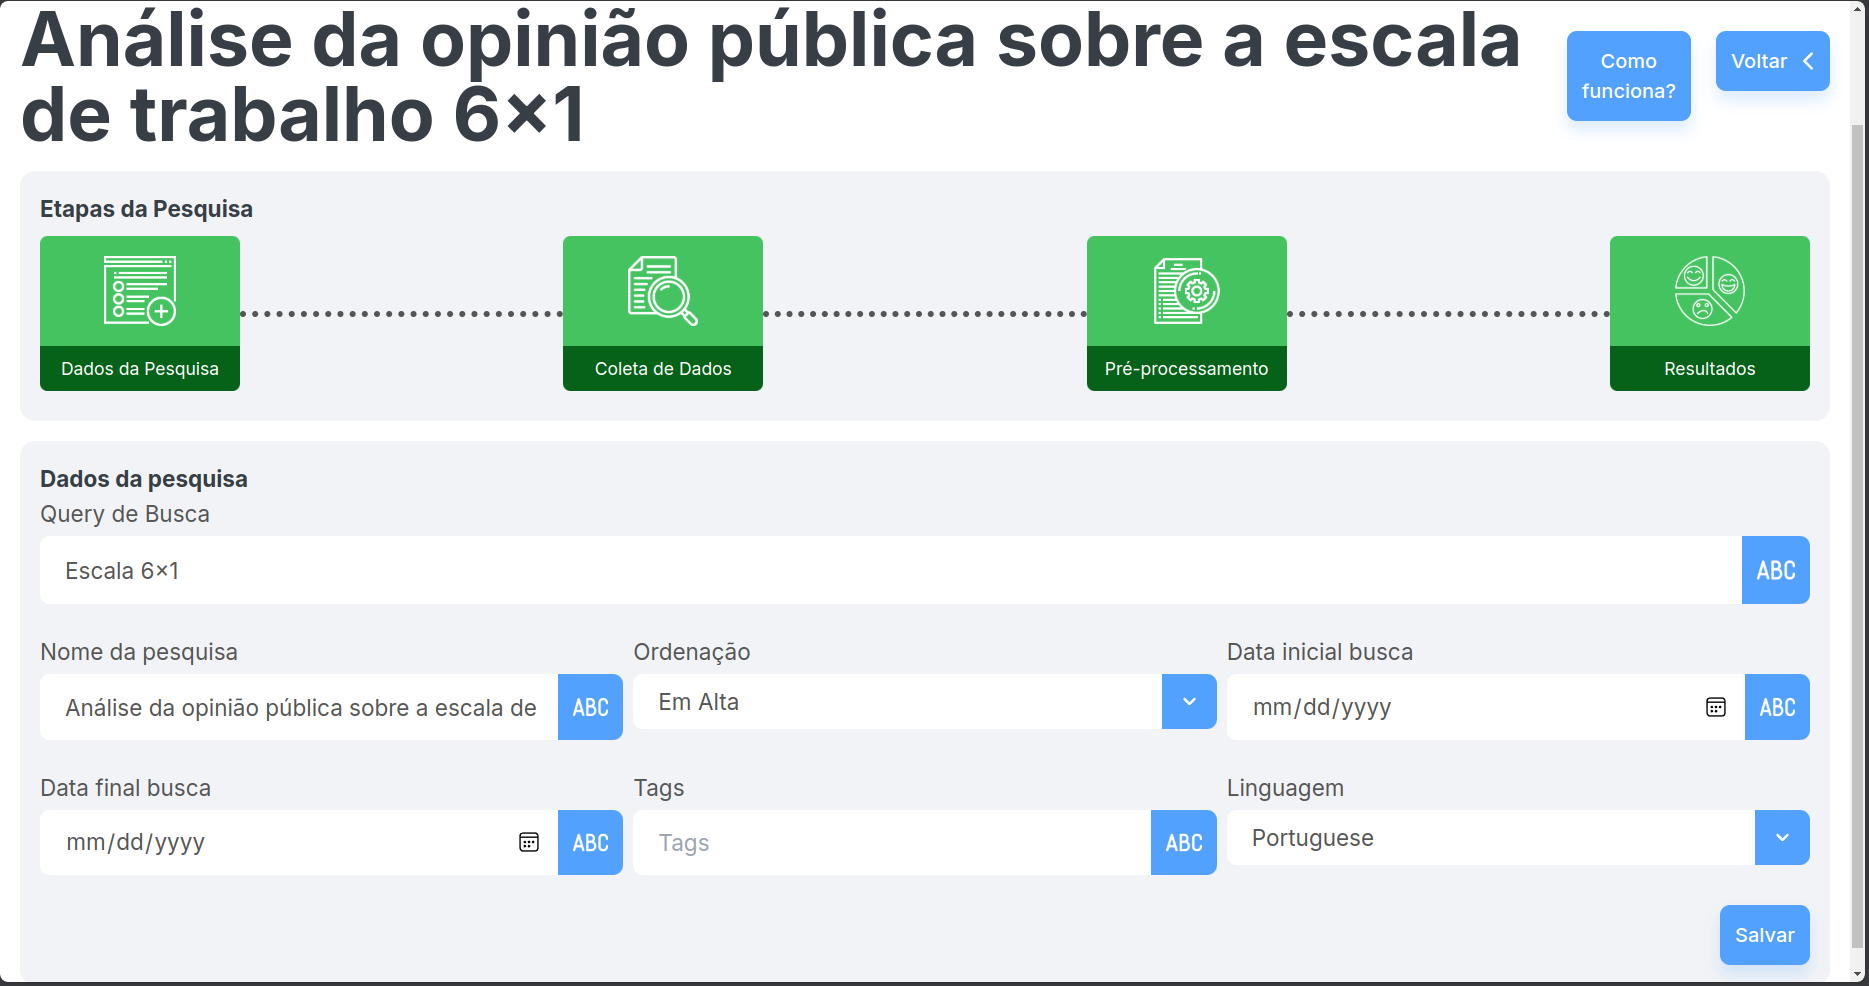
\includegraphics[scale=0.35]{imagens/sentilytics/estudo-caso/dados_pesquisa.png}
\end{center}
}
\legend{Fonte: Autor (2025).}
\end{figure}

Como podemos visualizar na \autoref{configuracao_pesquisa}, os
parâmetros de busca utilizados foram a query ``Escala 6x1'', sem a
aplicação de filtros de intervalo de datas. As postagens foram ordenadas
de acordo com sua popularidade, priorizando as mais relevantes dentro da
plataforma.

A pesquisa foi executada no dia 7 de fevereiro de 2025, onde no total
foram coletadas 4880 postagens. Esse volume de dados permite uma análise
representativa das percepções sobre a escala 6x1, abrangendo diferentes
perspectivas e experiências compartilhadas pelos usuários.

\hypertarget{pruxe9-processamento-dos-dados}{%
\subsection{Pré-processamento dos
Dados}\label{pruxe9-processamento-dos-dados}}

Após a coleta, os textos das postagens passaram por uma sequência de
tarefas de pré-processamento para garantir maior qualidade na análise.
Para isso um workflow foi criado com as tarefas que serão usadas para
realizar o pré-processamento, que podemos visualizar na
\autoref{pipeline_processamento}.

\begin{figure}[htbp]
\hypertarget{pipeline_processamento}{%
\caption{Workflow de pré-processamento}\label{pipeline_processamento}
\begin{center}
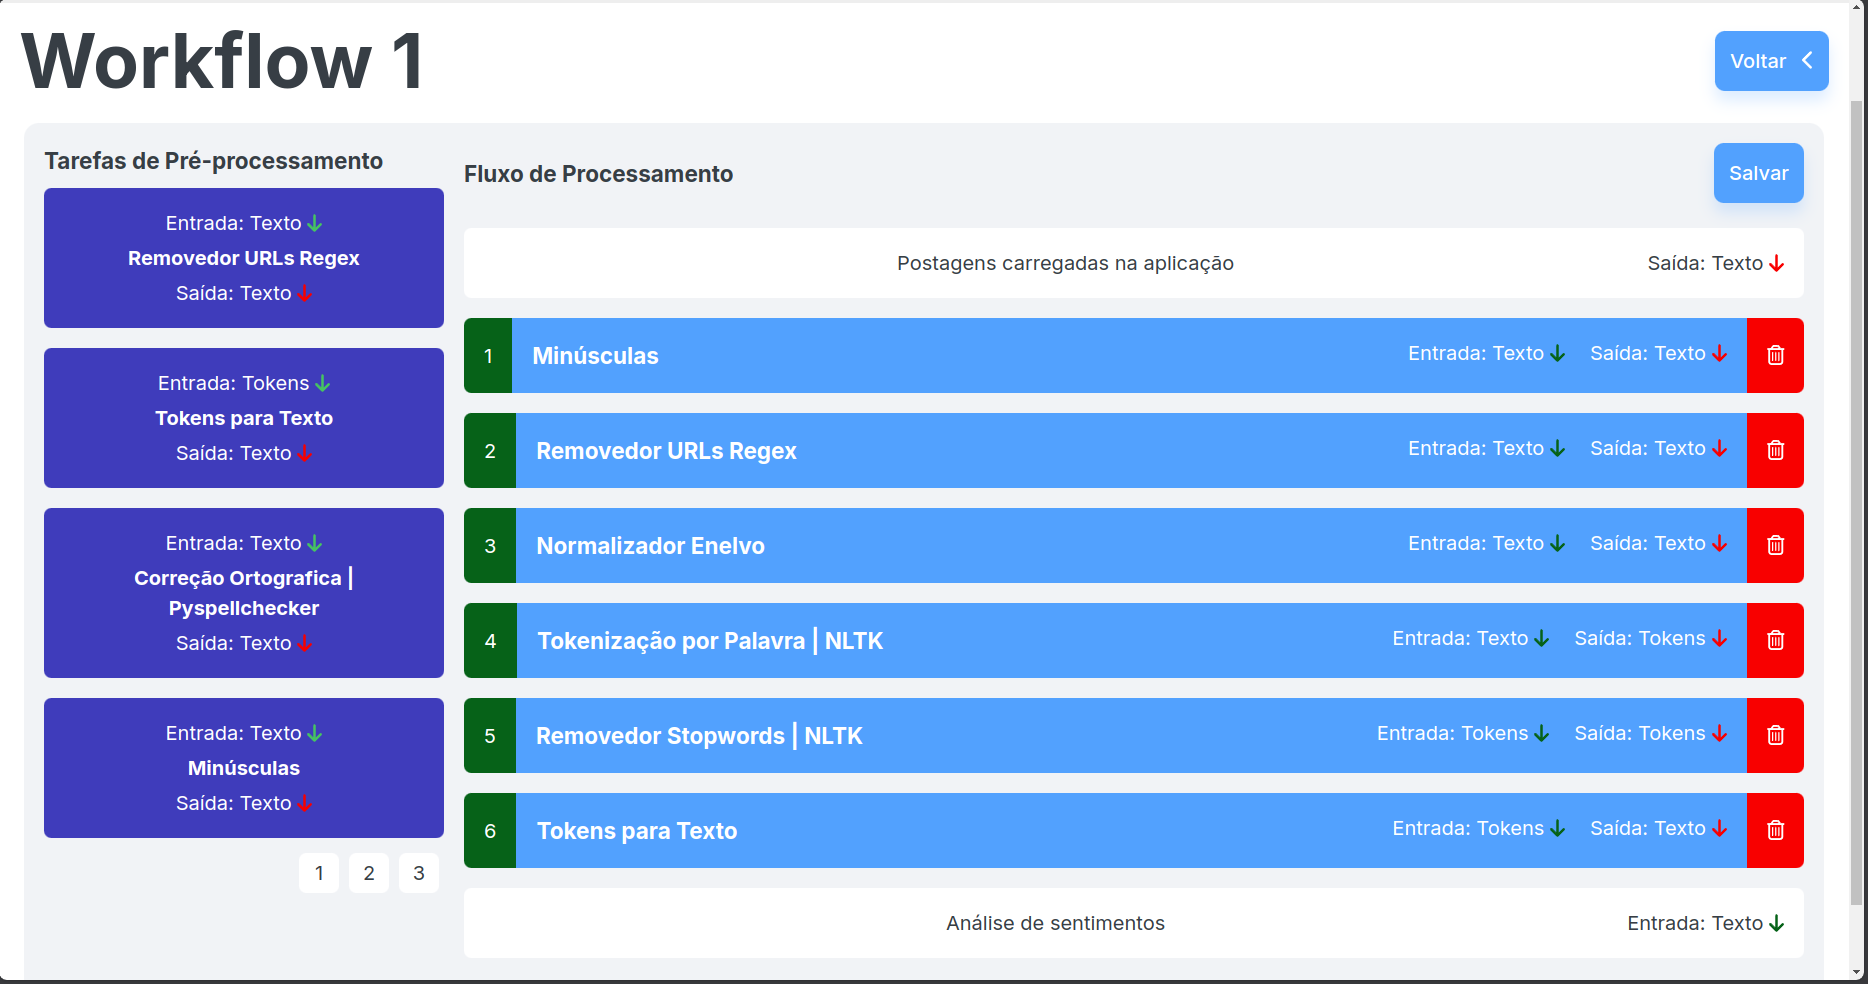
\includegraphics[scale=0.35]{imagens/sentilytics/estudo-caso/workflow.png}
\end{center}
}
\legend{Fonte: Autor (2025).}
\end{figure}

A \autoref{pipeline_processamento} mostra um conjunto de tarefas
organizadas em ordem, cada postagem vai passar por essas tarefas em
sequência, as tarefas são:

\begin{enumerate}
\def\labelenumi{\arabic{enumi})}
\tightlist
\item
  Minúsculas: Transformação de todo o texto para minúsculas, garantindo
  uniformidade;
\item
  Removedor URLs Regex: Remove URLs do texto;
\item
  Normalizador Enelvo: Normalização do texto para corrigir erros
  ortográficos e abreviações comuns;
\item
  Tokenização por Palavra \textbar{} NLTK: Segmentação do texto em
  palavras individuais (tokens);
\item
  Removedor Stopwords: Remoção de palavras irrelevantes que não
  contribuem para a análise do sentimento;
\item
  Tokens para Texto: Os tokens são unidos novamente formando uma frase
  novamente com os tokens separados por um espaço em branco.
\end{enumerate}

\hypertarget{anuxe1lise-de-sentimentos}{%
\subsection{Análise de Sentimentos}\label{anuxe1lise-de-sentimentos}}

Após o pré-processamento, as postagens foram submetidas ao modelo de
análise de sentimentos do Sentilytics, que utiliza o VADER\footnote{A
  documentação do VADER está disponível no link:
  \url{https://www.nltk.org/_modules/nltk/sentiment/vader.html}}
(Valence Aware Dictionary and sEntiment Reasoner), uma ferramenta da
biblioteca NLTK\footnote{O site do NLTK está disponível no link:
  \url{https://www.nltk.org/}} (Natural Language Toolkit). O VADER é um
modelo baseado em regras e léxicos, projetado especificamente para a
análise de sentimentos em textos informais.

Cada postagem recebeu uma pontuação de polaridade, categorizada em:

\begin{itemize}
\tightlist
\item
  Positivo: O quanto a postagem é positiva;
\item
  Neutro: O quanto a postagem é neutra;
\item
  Negativo: O quanto a postagem é negativa;
\item
  Composta: A pontuação composta consiste em um valor que representa a
  polaridade geral do texto, onde esse valor varia entre entre -1 (muito
  negativo) e +1 (muito positivo).
\end{itemize}

A pontuação composta é calculada a partir da soma das valências das
palavras presentes no texto. Essas valências são determinadas por um
léxico de sentimentos, que associa palavras ao score de polaridade
positiva e negativa. Além disso, a análise considera uma série de
heurísticas que ajustam o impacto dessas palavras com base no contexto
em que aparecem, como a presença de negações ou intensificadores.

Para garantir que os valores fiquem dentro do intervalo de -1 a +1, a
soma das valências é normalizada usando a seguinte fórmula:

\begin{equation}
    compound = \frac{sum_s}{\sqrt{sum_s^2 + \alpha}}
\end{equation}

\begin{itemize}
\tightlist
\item
  sum\_s é a soma das valências das palavras no texto;
\item
  \(\alpha\) é um fator de suavização que evita que textos muito longos
  tenham scores excessivamente altos ou baixos (o valor padrão no VADER
  é 15).
\end{itemize}

Com base nessa normalização, o sentilytics consegue interpretar o
sentimento predominante na postagem da seguinte forma:

\begin{itemize}
\tightlist
\item
  Se o score composto for maior ou igual a 0.05: O sentimento da
  postagem é considerado positivo;
\item
  Se for menor ou igual a -0.05: O sentimento é negativo;
\item
  Se estiver entre -0.05 e 0.05: O sentimento é neutro.
\end{itemize}

\hypertarget{anuxe1lise-gruxe1fica-e-textual-do-sentilytics}{%
\section{Análise gráfica e textual do
Sentilytics}\label{anuxe1lise-gruxe1fica-e-textual-do-sentilytics}}

Nesta seção, são apresentados os principais resultados obtidos com o
Sentilytics na análise de sentimentos sobre temas políticos no Bluesky.
A ferramenta gerou diferentes representações visuais, incluindo gráficos
de distribuição de sentimentos, nuvens de palavras e os posts mais
engajados. Além disso, \emph{insights} gerados por inteligência
artificial auxiliaram na interpretação dos dados, fornecendo resumos e
tendências detectadas automaticamente. A seguir, cada gráfico é
analisado individualmente, seguido de uma discussão geral sobre os
padrões observados e suas possíveis implicações.

\begin{figure}[htbp]
\hypertarget{grafico_numero_comentarios_por_sentimento}{%
\caption{Gráfico de Número de Comentários por Sentimentos}\label{grafico_numero_comentarios_por_sentimento}
\begin{center}
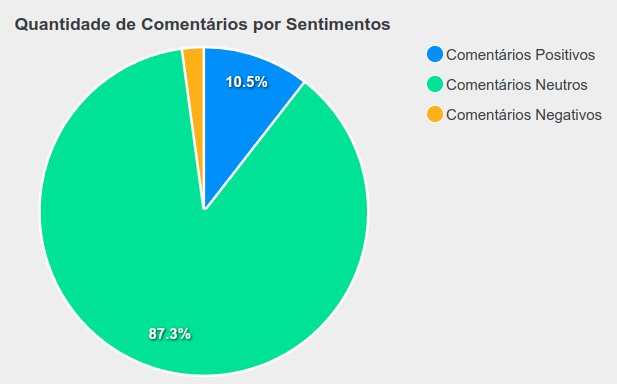
\includegraphics[scale=0.3]{imagens/sentilytics/estudo-caso/quantidade_comentarios_por_sentimentos.png}
\end{center}
}
\legend{Fonte: Autor (2025).}
\end{figure}

O gráfico apresentado na
\autoref{grafico_numero_comentarios_por_sentimento} exibe a distribuição
dos sentimentos nas postagens analisadas. Observa-se que a maioria das
postagens foi classificada como \textbf{neutra}, representando 87,3\% do
total. Já os sentimentos \textbf{positivos} correspondem a 10,5\%,
enquanto os \textbf{negativos} representam apenas 2,2\% das postagens.

No contexto político, o debate sobre a escala 6x1 ganhou destaque no
último ano, impulsionado pela apresentação de uma Proposta de Emenda à
Constituição (PEC) que propõe seu fim. A análise dos comentários
coletados revela que a maioria das postagens apresenta um tom neutro,
sugerindo que grande parte das discussões tem caráter informativo ou
analítico. No entanto, entre as postagens que expressam um viés
emocional, observa-se uma predominância de sentimentos positivos em
relação ao tema. Esse resultado indica que há uma inclinação favorável
da opinião pública quanto à possibilidade de alteração ou extinção da
escala 6x1, refletindo um possível apoio da população a mudanças na
organização da jornada de trabalho.

O Sentilytics também gerou um \emph{insight} baseado em AI para analisar
o resultado do gráfico, interpretando a predominância do sentimento de
neutralidade da seguinte forma: ``Em suma, a análise de sentimentos
revela uma necessidade de explorar mais a fundo as razões subjacentes ao
otimismo ou pessimismo contidos nos 512 comentários positivos e nos 105
negativos, bem como entender como estimular uma participação mais ativa
do público que se mostrou neutro.''.

Esse resultado sugere que, apesar da predominância de comentários
neutros, ainda existe a necessidade de entender melhor os sentimentos
positivos e negativos expressos pela população. O alto número de
postagens neutras pode ser interpretado como uma cautela do público em
relação ao tema, especialmente considerando que mudanças trabalhistas
costumam gerar incertezas. Esses \emph{insights} foram gerados
utilizando a API do ChatGPT, na qual os dados do gráfico em questão são
enviados para o modelo, que então realiza uma análise.

Embora os resultados apresentados forneçam uma visão geral sobre a
distribuição dos sentimentos, é importante considerar as limitações
inerentes ao modelo de análise utilizado. A predominância de comentários
classificados como neutros pode indicar uma limitação da ferramenta,
decorrente do uso de um modelo baseado em léxicos.

\begin{figure}[htbp]
\hypertarget{grafico_media_engajamento}{%
\caption{Gráfico da Média de Engajamento por Sentimentos}\label{grafico_media_engajamento}
\begin{center}
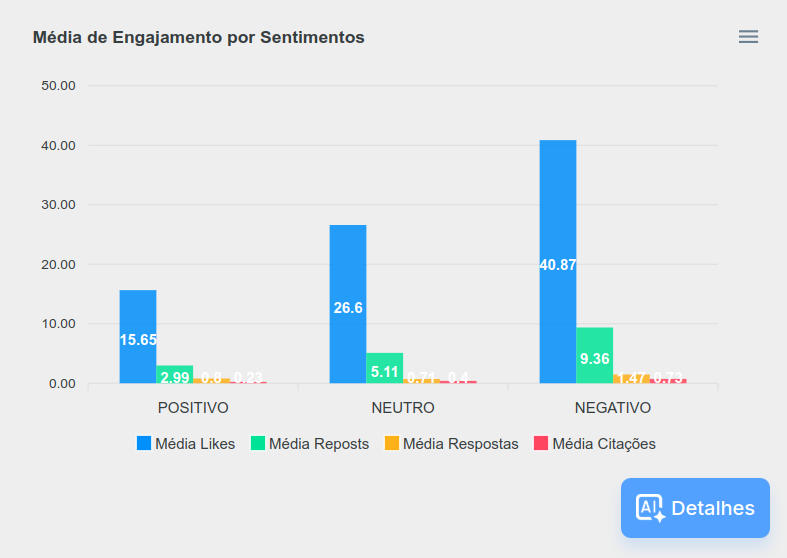
\includegraphics[scale=0.3]{imagens/sentilytics/estudo-caso/media_engajamento_por_sentimento.png}
\end{center}
}
\legend{Fonte: Autor (2025).}
\end{figure}

Na \autoref{grafico_media_engajamento}, é apresentado um gráfico de
barras que ilustra a média de engajamento por sentimento, considerando
as interações dos usuários, como likes, repostagens, respostas e
citações. Cada barra no gráfico representa a média calculada para um
tipo específico de interação, agrupada de acordo com os sentimentos
Positivo, Negativo e Neutro.

A análise desse gráfico permite identificar qual categoria de sentimento
gera maior engajamento geral, bem como tendências específicas por tipo
de interação. Por exemplo, é possível observar se posts com sentimentos
negativos recebem mais repostagens, indicando maior disseminação de
conteúdos críticos.

A análise do gráfico da \autoref{grafico_media_engajamento} revela que
os sentimentos negativos geraram o maior engajamento geral,
destacando-se especialmente pela média de likes e reposts. Esse padrão
sugere que conteúdos críticos ou de tom negativo tendem a atrair mais
atenção e interação do público, possivelmente devido à inclinação dos
usuários em amplificar mensagens com caráter negativo ou polarizador.

\begin{figure}[htbp]
\hypertarget{grafico_total_engajamento}{%
\caption{Gráfico da Total de Engajamento por Sentimentos}\label{grafico_total_engajamento}
\begin{center}
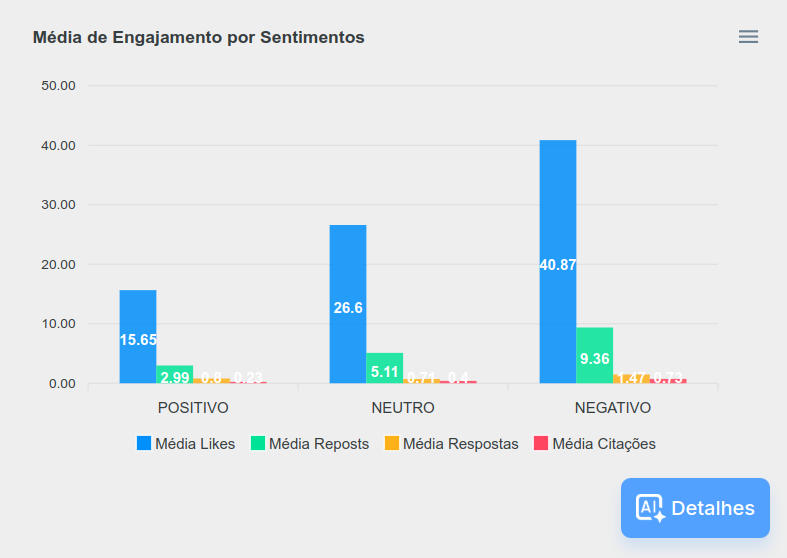
\includegraphics[scale=0.3]{imagens/sentilytics/estudo-caso/media_engajamento_por_sentimento.png}
\end{center}
}
\legend{Fonte: Autor (2025).}
\end{figure}

O gráfico apresentado na \autoref{grafico_total_engajamento} exibe o
total de interações por sentimento, podemos interpretar esse gráfico
observando quais sentimentos geram o maior volume absoluto de
engajamento, bem como identificar padrões na distribuição das interações
por tipo. Ao contrário do gráfico da \autoref{grafico_media_engajamento}
que mostra a média, este gráfico analisa o impacto acumulado das
interações em cada categoria de sentimento.

Os resultados apresentados no gráfico mostram que postagens com
sentimento neutro tiveram um engajamento significativamente maior em
todas as métricas analisadas. Esse padrão indica que conteúdos
classificados como neutros possuem um impacto acumulado mais alto,
possivelmente devido à maior quantidade de postagens nesta categoria.
Por outro lado, ao comparar os sentimentos negativos e positivos podemos
notar que o sentimento negativo gera um volume maior de repostagens.

\begin{figure}[htbp]
\hypertarget{grafico_analise_temporal}{%
\caption{Gráfico da Análise Temporal de Sentimentos}\label{grafico_analise_temporal}
\begin{center}
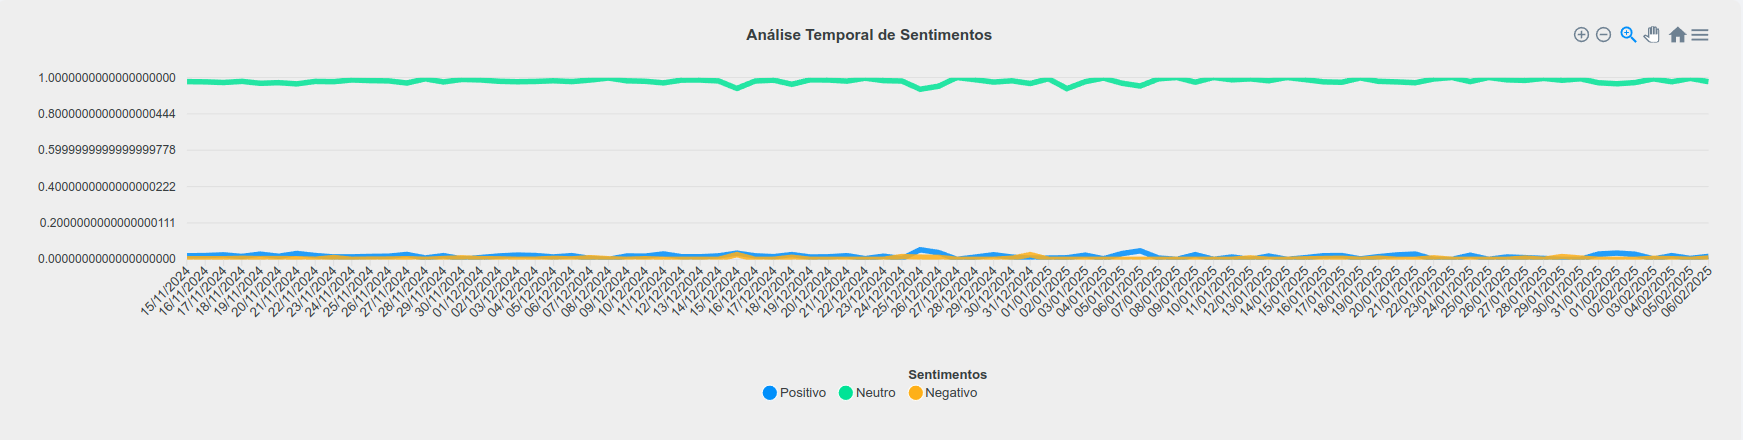
\includegraphics[scale=0.26]{imagens/sentilytics/estudo-caso/analise_temporal_sentimentos.png}
\end{center}
}
\legend{Fonte: Autor (2025).}
\end{figure}

O gráfico apresentado na \autoref{grafico_analise_temporal} exibe a
evolução dos níveis de sentimento (Positivo, Negativo e Neutro) ao longo
de um período de dias. Cada ponto no gráfico representa o valor médio do
sentimento para aquele dia, variando entre 0 e 1, onde valores mais
próximos de 1 indicam uma maior intensidade do sentimento correspondente
nas postagens analisadas.

Esse tipo de gráfico é útil para identificar tendências temporais no
comportamento emocional das postagens, permitindo observar oscilações
nos sentimentos predominantes durante eventos específicos ou mudanças
graduais no tom das interações ao longo do tempo.

A partir da análise do gráfico da \autoref{grafico_analise_temporal},
podemos identificar que o sentimento neutro se mantém em uma linha
estável, possuindo menos variações, o que é coerente com o que vimos em
análise anteriores. Em relação a análise dos sentimentos positivos e
negativos, podemos visualizar mais variações marcadas e pontuais, com
picos em alguns dias específicos.

\begin{figure}[htbp]
\hypertarget{nuvem_palavras}{%
\caption{Nuvem de Palavras}\label{nuvem_palavras}
\begin{center}
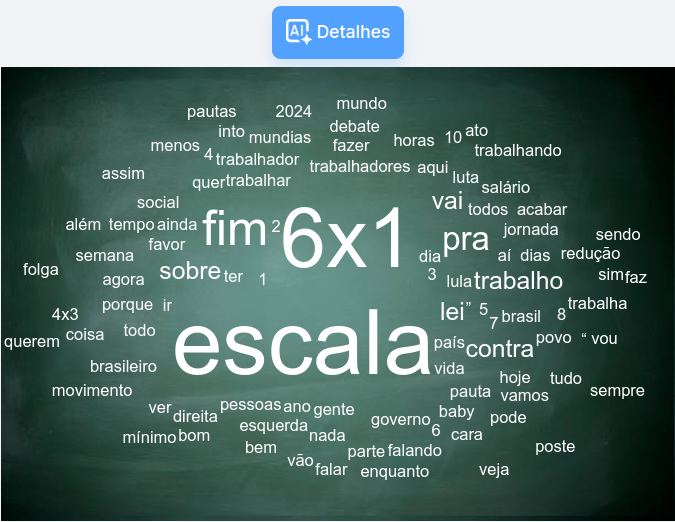
\includegraphics[scale=0.4]{imagens/sentilytics/estudo-caso/bag_of_words.png}
\end{center}
}
\legend{Fonte: Autor (2025).}
\end{figure}

Na \autoref{nuvem_palavras} podemos visualizar a nuvem de palavras
gerada na aplicação, ela mostra as palavras mais frequentes nos textos
analisados, sendo baseada no texto pré-processado. Isso significa que
elementos irrelevantes foram removidos (como stopwords), e apenas os
termos significativos foram mantidos. A frequência de cada palavra
determina o destaque que ela recebe na nuvem, permitindo identificar
rapidamente os principais tópicos e padrões debatidos pelos usuários.

A análise da nuvem de palavras reforça que a discussão sobre o fim da
escala 6x1 é central e polarizadora, com ``escala'' (5.365 ocorrências)
e ``6x1'' (5.020 ocorrências) sendo os termos mais frequentes, seguidos
por ``fim'' (2.229 ocorrências). Isso demonstra o foco principal no
impacto e nas mudanças associadas à proposta.

Os termos ``contra'' (894 ocorrências) sugere uma oposição ou apoio
ativo à pauta, indicando que a comunidade está dividida entre grupos que
defendem ou rejeitam o fim da escala. Além disso, palavras como
``trabalho'' (529 ocorrências), ``trabalhadores'' (268 ocorrências) e
``jornada'' (134 ocorrências) indicam que a discussão também foca nos
impactos diretos sobre a rotina e os direitos dos trabalhadores.

A presença de palavras como ``governo'' (257 ocorrências), ``direita''
(230 ocorrências) e ``esquerda'' (256 ocorrências) sugere que o debate
não é apenas técnico ou econômico, mas também politizado, com diferentes
ideologias influenciando as percepções públicas sobre o tema.

Por fim, termos como ``luta'' (243 ocorrências) e ``vida'' (253
ocorrências) reforçam o caráter emocional do discurso, destacando que
essa proposta é vista como algo que impacta diretamente a qualidade de
vida e as condições de trabalho da população. Diante desse cenário, a
análise gerada por IA (Inteligência Artificial) na aplicação oferece uma
interpretação dos dados, ajudando a contextualizar esses padrões e
fornecendo \emph{insights} sobre como o público está reagindo ao debate.

\begin{figure}[htbp]
\hypertarget{top_posts_engajados}{%
\caption{Top posts Engajados}\label{top_posts_engajados}
\begin{center}
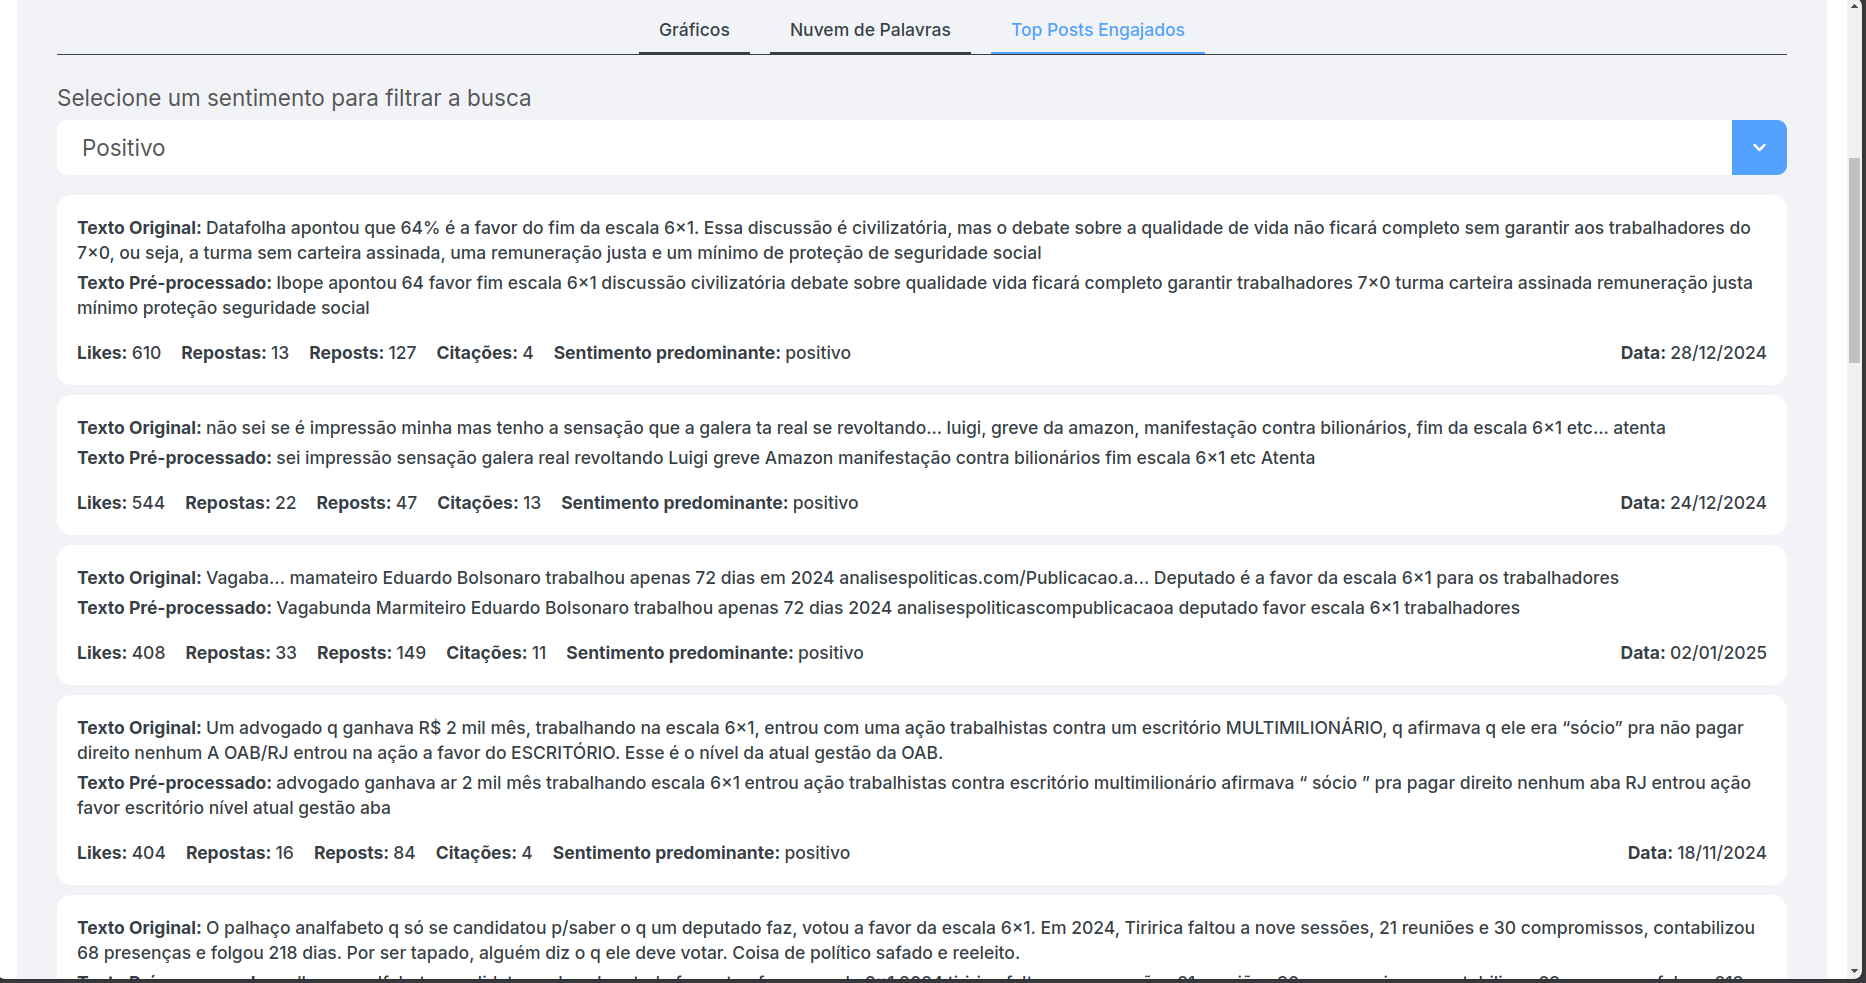
\includegraphics[scale=0.3]{imagens/sentilytics/estudo-caso/top_posts_engajados.png}
\end{center}
}
\legend{Fonte: Autor (2025).}
\end{figure}

A tela apresentada na \autoref{top_posts_engajados} exibe os top posts
com maior engajamento, permitindo uma análise detalhada das postagens
mais populares no contexto da pesquisa. Essa funcionalidade organiza os
posts ranqueados com base na soma total de interações realizadas pelo
usuário, apresentados de forma decrescente para destacar os conteúdos
que mais mobilizaram o público.

A aplicação também oferece a funcionalidade de aplicar filtros por
sentimento (Positivo, Neutro e Negativo), permitindo que o usuário
identifique facilmente quais tipos de conteúdos geraram mais interação
em cada categoria emocional. Além disso, é possível visualizar tanto o
texto original do post quanto sua versão pré-processada, facilitando a
compreensão de como as etapas de processamento (como remoção de
stopwords ou normalização) impactaram a análise. Essa funcionalidade
possibilita que o usuário valide os resultados obtidos e compreenda de
forma mais aprofundada os padrões de engajamento associados a cada tipo
de postagem.

A funcionalidade de top posts engajados, com a visualização do texto
original e pré-processado, representa uma ferramenta importante para
analisar como a audiência responde a conteúdos emocionais, informativos
ou polêmicos, oferecendo uma visão prática e direta dos dados
processados pela aplicação.

\hypertarget{limitauxe7uxf5es-do-estudo-de-caso}{%
\subsection{Limitações do Estudo de
Caso}\label{limitauxe7uxf5es-do-estudo-de-caso}}

Embora o presente estudo tenha alcançado seus objetivos principais, é
importante reconhecer algumas limitações que podem ter impactado os
resultados e a abrangência da análise. Essas limitações estão
relacionadas tanto à aplicação Sentilytics quanto ao escopo do estudo de
caso, e incluem:

\begin{enumerate}
\def\labelenumi{\arabic{enumi})}
\item
  \textbf{Integração limitada à rede social Bluesky}: Atualmente, o
  Sentilytics está integrado apenas à rede social Bluesky, uma
  plataforma que ainda não possui grande relevância no Brasil e é pouco
  utilizada em comparação com outras redes sociais, como X (Antigo
  Twitter) e Facebook. Essa limitação reduz a representatividade da
  análise, já que os dados coletados refletem um público menor e
  potencialmente menos diversificado;
\item
  Opções limitadas de pré-processamento e análise de sentimentos: O
  Sentilytics oferece atualmente um número reduzido de tarefas de
  pré-processamento e utiliza apenas o VADER como modelo de análise de
  sentimentos. Embora o formato atual da aplicação permita a adição de
  outras funções sem a necessidade de alterações significativas, essas
  limitações podem impactar a qualidade dos resultados, especialmente
  para textos em português, onde o VADER tem dificuldades em captar
  nuances emocionais, como ironia e sarcasmo;
\item
  Tamanho da amostra de dados: O estudo considerou uma amostra de 4.880
  postagens coletadas no Bluesky. Embora seja suficiente para uma
  análise inicial, um número maior de postagens poderia fornecer uma
  visão mais abrangente e robusta sobre os padrões de engajamento e os
  sentimentos expressos pela audiência;
\item
  Viés na análise de sentimentos: O modelo de análise de sentimentos
  utilizado, o VADER, apresenta limitações conhecidas, como dificuldade
  para interpretar ironias, sarcasmos e textos altamente subjetivos, o
  que é comum em postagens de redes sociais. Isso pode ter levado a uma
  classificação imprecisa em alguns casos, especialmente nas postagens
  que dependem de contextos mais complexos para serem interpretadas
  corretamente;
\item
  Dados reais não rotulado para comparação: Os dados são reais e obtidos
  diretamente da rede social, portanto, não foram rotulados por
  especialistas, a fim de analisar a acurácia e precisão dos resultados.
\end{enumerate}

Essas limitações não comprometem os objetivos gerais do estudo, mas
indicam possibilidades de melhoria para pesquisas futuras. A ampliação
da integração do Sentilytics para outras redes sociais, a implementação
de modelos mais robustos de análise de sentimentos, como redes neurais
treinadas especificamente para o português, e o aumento do volume de
dados analisados podem contribuir para resultados ainda mais precisos e
abrangentes.

\hypertarget{considerauxe7uxf5es-finais}{%
\chapter{Considerações Finais}\label{considerauxe7uxf5es-finais}}

As redes sociais desempenham um papel essencial na compreensão da
opinião pública, influenciando debates políticos, decisões econômicas e
o comportamento das novas gerações. A análise de sentimentos nessas
plataformas tornou-se uma ferramenta indispensável para identificar
tendências, polarizações e padrões emocionais que impactam diferentes
setores. No entanto, as soluções existentes frequentemente apresentam
barreiras técnicas, exigindo conhecimentos avançados para a coleta e o
processamento dos dados, além de nem sempre oferecerem integração direta
com redes sociais. Essa limitação dificulta o acesso de pesquisadores e
analistas que necessitam de um processo mais intuitivo e automatizado
para interpretar grandes volumes de dados de forma eficiente.

Diante desse desafio, o Sentilytics foi desenvolvido como uma solução
integrada e automatizada para análise de sentimentos, permitindo a
coleta, o pré-processamento e a classificação dos dados de forma
personalizável. Sua integração direta com redes sociais e o suporte à
configuração de workflows de pré-processamento garantem maior
flexibilidade e acessibilidade, mesmo para usuários sem experiência
técnica avançada. A ferramenta foi validada por meio de um estudo de
caso sobre o debate do fim da escala 6x1, demonstrando sua capacidade de
extrair \emph{insights} relevantes a partir de postagens públicas. Com
isso, o Sentilytics se posiciona como uma alternativa inovadora para a
análise de sentimentos no contexto digital, contribuindo para estudos
acadêmicos, monitoramento de redes e tomada de decisões estratégicas em
diversas áreas.

A ferramenta proposta demonstrou sua eficácia ao permitir a configuração
de workflows personalizados de pré-processamento, garantindo maior
flexibilidade aos usuários na análise de dados. Além disso, sua
integração com o Bluesky possibilitou a obtenção de postagens de forma
gratuita, superando as limitações impostas por redes sociais com acesso
pago às suas APIs. Os resultados evidenciaram padrões relevantes na
opinião pública, reforçando o potencial da solução para aplicações em
pesquisas acadêmicas, análise de tendências sociais e monitoramento de
redes.

Entretanto, algumas limitações foram identificadas. A dependência
exclusiva do modelo VADER pode comprometer a precisão da análise em
determinados contextos, especialmente ao lidar com ironia e ambiguidades
que são comumente observados em textos nas redes sociais. Além disso, a
restrição ao Bluesky reduz a abrangência dos dados coletados, uma vez
que a plataforma ainda possui baixa adesão no Brasil em comparação com
outras redes sociais.

Atualmente, os dados gerados oferecem uma visão geral da análise de
sentimentos, porém, há oportunidades para aprimorar a forma como essas
informações são exibidas, tornando-as mais intuitivas e acessíveis para
diferentes perfis de usuários. Melhorias na organização dos gráficos, na
personalização dos relatórios e na inclusão de explicações automáticas
sobre os resultados poderiam tornar a interpretação dos \emph{insights}
mais clara e direta.

Para trabalhos futuros, propõe-se a expansão da ferramenta com a
integração de novos modelos de análise de sentimentos, incluindo
técnicas baseadas em aprendizado profundo (Deep Learning), que podem
melhorar a acurácia da classificação. Atualmente, a aplicação já permite
a adição simplificada de novas tarefas de pré-processamento. A ideia é
utilizar esse fluxo para incorporar diferentes modelos e algoritmos de
análise de sentimentos, tornando o sistema mais robusto e flexível.

A inclusão do suporte a múltiplas redes sociais tornaria o sistema mais
abrangente. Redes como Twitter e Reddit poderiam ser adicionadas como
fontes de dados, ampliando a diversidade de conteúdos analisados.
Atualmente, a autenticação na aplicação é feita exclusivamente pelo
Bluesky. Para viabilizar a integração com outras redes, a ferramenta
passaria a contar com um sistema de cadastro e autenticação próprios,
permitindo que os usuários informem suas credenciais apenas no momento
da coleta de dados em cada rede social.

Outra possível melhoria é a adoção de métodos mais avançados de
pré-processamento, capazes de lidar com nuances linguísticas e melhorar
a qualidade da análise textual. Essas evoluções tornarão a ferramenta
ainda mais versátil e aplicável a diferentes domínios, consolidando sua
contribuição para o campo da análise de sentimentos em redes sociais.
Atualmente, a modularização da aplicação já permite a adição de novas
tarefas de pré-processamento de maneira simplificada.

Por fim, a implementação de um painel de administração também seria um
avanço importante. Atualmente, para disponibilizar novas tarefas de
pré-processamento aos usuários, é necessário configurar manualmente
essas funções na base de dados. A inclusão de uma interface
administrativa permitiria que essa configuração fosse realizada de
maneira mais intuitiva, otimizando o gerenciamento das funcionalidades
da plataforma.

% ----------------------------------------------------------
% ELEMENTOS PÓS-TEXTUAIS
% ----------------------------------------------------------
\postextual
% ----------------------------------------------------------

% ----------------------------------------------------------
% Início dos ELEMENTOS PÓS-TEXTUAIS
% ----------------------------------------------------------
\postextual
% ----------------------------------------------------------

% ----------------------------------------------------------
% Referências bibliográficas
% ----------------------------------------------------------
\bibliography{xxx-referencias}
\bibliographystyle{abntex2-alf.bst}
% ----------------------------------------------------------
% Apêndices
% ----------------------------------------------------------
%% 
% Seção de apendices configurada como desativada
%% 
% ---

% ----------------------------------------------------------
% Anexos desativados: 
% Seção de anexos configurada como desativada
% ----------------------------------------------------------



\end{document}
